% !TeX TXS-program:compile = txs:///pdflatex/[--shell-escape]
% speciální nastavení pro TeXstudio kvůli balíčku minted

%==============================================================================
% tento soubor pouzijte jako zaklad
% this file should be used as a base for the thesis
% Autoři / Authors: 2008 Michal Bidlo, 2016 Jaroslav Dytrych


% Kontakt pro dotazy a připomínky: dytrych@fit.vutbr.cz
% Contact for questions and comments: dytrych@fit.vutbr.cz
%==============================================================================
% kodovaní: UTF-8 (zmena prikazem iconv, recode nebo cstocs)
% encoding: UTF-8 (you can change it by command iconv, recode or cstocs)
%------------------------------------------------------------------------------
% zpracování / processing: make, make pdf, make clean
%==============================================================================
% Soubory, které je nutné upravit: / Files which have to be edited:
%   projekt-20-literatura-bibliography.bib - literatura / bibliography
%   projekt-01-kapitoly-chapters.tex - obsah práce / the thesis content
%   projekt-30-prilohy-appendices.tex - přílohy / appendices
%==============================================================================
\documentclass[zadani,print]{fitthesis} % bez zadání - pro začátek práce, aby nebyl problém s překladem
%\documentclass[english]{fitthesis} % without assignment - for the work start to avoid compilation problem
%\documentclass[zadani]{fitthesis} % odevzdani do wisu - odkazy jsou barevné
%\documentclass[english,zadani]{fitthesis} % for submission to the IS FIT - links are color
%\documentclass[zadani,print]{fitthesis} % pro tisk - odkazy jsou černé
%\documentclass[english,zadani,print]{fitthesis} % for the print - links are black
% * Je-li prace psana v anglickem jazyce, je zapotrebi u tridy pouzit 
%   parametr english nasledovne:
%   If thesis is written in english, it is necessary to use 
%   parameter english as follows:
%      \documentclass[english]{fitthesis}
% * Je-li prace psana ve slovenskem jazyce, je zapotrebi u tridy pouzit 
%   parametr slovak nasledovne:
%      \documentclass[slovak]{fitthesis}

% Základní balíčky jsou dole v souboru šablony fitthesis.cls
% Basic packages are at the bottom of template file fitthesis.cls

%zde muzeme vlozit vlastni balicky / you can place own packages here

%footnote in caption for figure
\usepackage{graphicx} % vkládání obrázků
\usepackage{afterpage}

%subfigure
\usepackage{caption}
\usepackage{subcaption}

%item/enumerate
\usepackage{enumitem} % umožňuje nastavit menší mezery mezi odrážkami
%\usepackage{enumerate} % umožňuje širší možnosti nastavení enumerate pomoci [-]

%využito v tabulce, která označuje, co které prostředí splňuje a co ne
\usepackage{bbding} % kvůli znakům fajka (\CheckmarkBold) a křížek (\XSolidBrush) => \Has a \NoHas


%---rm---------------
\renewcommand{\rmdefault}{lmr}%zavede Latin Modern Roman jako rm / set Latin Modern Roman as rm
%---sf---------------
\renewcommand{\sfdefault}{qhv}%zavede TeX Gyre Heros jako sf
%---tt------------
\renewcommand{\ttdefault}{lmtt}% zavede Latin Modern tt jako tt

% vypne funkci šablony, která automaticky nahrazuje uvozovky,
% aby nebyly prováděny nevhodné náhrady v popisech API apod.
% disables function of the template which replaces quotation marks
% to avoid unnecessary replacements in the API descriptions etc.
\csdoublequotesoff

% =======================================================================
% balíček "hyperref" vytváří klikací odkazy v pdf, pokud tedy použijeme pdflatex
% problém je, že balíček hyperref musí být uveden jako poslední, takže nemůže
% být v šabloně
% "hyperref" package create clickable links in pdf if you are using pdflatex.
% Problem is that this package have to be introduced as the last one so it 
% can not be placed in the template file.
\ifWis
\ifx\pdfoutput\undefined % nejedeme pod pdflatexem / we are not using pdflatex
\else
  \usepackage{color}
  \usepackage[unicode,colorlinks,hyperindex,plainpages=false,pdftex]{hyperref}
  \definecolor{links}{rgb}{0.4,0.5,0}
  \definecolor{anchors}{rgb}{1,0,0}
  \def\AnchorColor{anchors}
  \def\LinkColor{links}
  \def\pdfBorderAttrs{/Border [0 0 0] }  % bez okrajů kolem odkazů / without margins around links
  \pdfcompresslevel=9
\fi
\else % pro tisk budou odkazy, na které se dá klikat, černé / for the print clickable links will be black
\ifx\pdfoutput\undefined % nejedeme pod pdflatexem / we are not using pdflatex
\else
  \usepackage{color}
  \usepackage[unicode,colorlinks,hyperindex,plainpages=false,pdftex,urlcolor=black,linkcolor=black,citecolor=black]{hyperref}
  \definecolor{links}{rgb}{0,0,0}
  \definecolor{anchors}{rgb}{0,0,0}
  \def\AnchorColor{anchors}
  \def\LinkColor{links}
  \def\pdfBorderAttrs{/Border [0 0 0] } % bez okrajů kolem odkazů / without margins around links
  \pdfcompresslevel=9
\fi
\fi
% Řešení problému, kdy klikací odkazy na obrázky vedou za obrázek
% This solves the problems with links which leads after the picture
\usepackage[all]{hypcap}

% Informace o práci/projektu / Information about the thesis
%---------------------------------------------------------------------------
\projectinfo{
  %Prace / Thesis
  project=BP,            %typ prace BP/SP/DP/DR  / thesis type (SP = term project)
  year=2017,             %rok odevzdání / year of submission
  date=\today,           %datum odevzdani / submission date
  %Nazev prace / thesis title
  title.cs={
Lego Mindstorm EV3 ve výuce programování a robotiky},  %nazev prace v cestine ci slovenstine (dle zadani) / thesis title in czech language (according to assignment)
  title.en={Lego Mindstorm EV3 in Education of Programming and Robotics}, %nazev prace v anglictine / thesis title in english
  %Autor / Author
  author={Jaroslav Páral},   %cele jmeno a prijmeni autora / full name and surname of the author
  author.name={Jaroslav},   %jmeno autora (pro citaci) / author name (for reference) 
  author.surname={Páral},   %prijmeni autora (pro citaci) / author surname (for reference) 
  %author.title.p=Bc., %titul pred jmenem (nepovinne) / title before the name (optional)
  %author.title.a=PhD, %titul za jmenem (nepovinne) / title after the name (optional)
  %Ustav / Department
  department=UITS, % doplnte prislusnou zkratku dle ustavu na zadani: UPSY/UIFS/UITS/UPGM
  %                  fill in appropriate abbreviation of the department according to assignment: UPSY/UIFS/UITS/UPGM
  %Skolitel / supervisor
  supervisor={Filip Orság}, %cele jmeno a prijmeni skolitele / full name and surname of the supervisor
  supervisor.name={Filip},   %jmeno skolitele (pro citaci) / supervisor name (for reference) 
  supervisor.surname={Orság},   %prijmeni skolitele (pro citaci) / supervisor surname (for reference) 
  supervisor.title.p=Ing.,   %titul pred jmenem (nepovinne) / title before the name (optional)
  supervisor.title.a={Ph.D.},    %titul za jmenem (nepovinne) / title after the name (optional)
  %Klicova slova, abstrakty, prohlaseni a podekovani je mozne definovat 
  %bud pomoci nasledujicich parametru nebo pomoci vyhrazenych maker (viz dale)
  %Keywords, abstracts, declaration and acknowledgement can be defined by following 
  %parameters or using dedicated macros (see below)
  %===========================================================================
  %Klicova slova / keywords
  %keywords.cs={Klíčová slova v českém jazyce.}, %klicova slova v ceskem ci slovenskem jazyce
  %                                              keywords in czech or slovak language
  %keywords.en={Klíčová slova v anglickém jazyce.}, %klicova slova v anglickem jazyce / keywords in english
  %Abstract
  %abstract.cs={Výtah (abstrakt) práce v českém jazyce.}, % abstrakt v ceskem ci slovenskem jazyce
  %                                                         abstract in czech or slovak language
  %abstract.en={Výtah (abstrakt) práce v anglickém jazyce.}, % abstrakt v anglickem jazyce / abstract in english
  %Prohlaseni / Declaration
  %declaration={Prohlašuji, že jsem tuto bakalářskou práci vypracoval samostatně pod vedením pana ...},
  %Podekovani (nepovinne) / Acknowledgement (optional)
  %acknowledgment={Zde je možné uvést poděkování vedoucímu práce a těm, kteří poskytli odbornou pomoc.} % nepovinne
  %acknowledgment={Here it is possible to express thanks to the supervisor and to the people which provided professional help.} % optional
}

% Definice vlastních maker / own macros

\newcommand{\lego}{LEGO}
\newcommand{\lega}{LEGO}
\newcommand{\legoM}{LEGO MINDSTORMS}
\newcommand{\legoNXT}{LEGO MINDSTORMS NXT}
\newcommand{\legoEV}{LEGO MINDSTORMS EV3}
\newcommand{\legoSW}{LEGO MINDSTORMS EV3 Software}
\newcommand{\EVthree}{EV3}
\newcommand{\mindstorms}{MINDSTORMS}

\newcommand{\fll}{{\it FIRST} LEGO League}
\newcommand{\brick}{{\it Brick}}
\newcommand{\EVbrick}{EV3 {\it Brick}}
\newcommand{\EVblocks}{{\it programovací bloky}}


\newcommand{\evThreeDev}{{\it ev3dev}}
\newcommand{\leJOS}{{leJOS}}
\newcommand{\evRT}{{EV3RT}}

\newcommand{\NI}{National Instruments}
\newcommand{\labview}{LabVIEW}

\newcommand{\fischerT}{{\it fischertechnik}}
\newcommand{\FischerT}{{\it Fischertechnik}}

\newcommand{\merkur}{Merkur}

\newcommand{\arduino}{Arduino}

\newcommand{\Has}{\textcolor{green}{\CheckmarkBold}}
\newcommand{\NoHas}{\textcolor{red}{\XSolidBrush}}

%Abstrakt (cesky, slovensky ci anglicky) / Abstract (in czech, slovak or english)
\abstract[cs]{Bakalářská práce řeší problematiku vývoje softwaru pro \legoEV{}~\brick{}. 
Cílem je umožnit začínajícím programátorům vytvářet i~složitější programy, které již nelze jednoduše navrhnout ve~standardním prostředí. 
Práce porovnává dostupné platformy a~na základě výskledků testů vybírá jako nejlepší systém EV3RT. 
Součástí je návrh objektového API, které snižuje obtížnost přechodu z~originálního systému.
Zároveň poskytuje vhodnou platformu uživatelům, kterým již standardní vývojové prostředí dodávané se stavebnicí nedostačuje a~hledají výkonnější alternativu.}
\abstract[en]{In this bachelor thesis, we tackle the problem of software development for the Lego EV3 brick. We want to allow the beginner programmers to create complex programs that cannot be easily created using the original graphical programming interface.
We provide comparison of several alternatives of the original system from performance and user point of view. Based on this comparison, we choose EV3RT as base for our work.
We also present our object-oriented API built on top of the EV3RT system to ease the transfer from graphical to text programming. Therefore, we provide a suitable platform for the beginners, who already reached the limits of standard system and want to develop more complex programs demanding more computing power.
}

%Klicova slova (cesky, slovensky ci anglicky) / Keywords (in czech, slovak or english)
\keywords[cs]{\legoEV, programovací platformy, ev3dev, Matlab, ROBOTC,  ROS, EV3RT, ev3cxx}
\keywords[en]{\legoEV, programing platforms, ev3dev, Matlab, ROBOTC,  ROS, EV3RT, ev3cxx}

%Prohlaseni (u anglicky psane prace anglicky, u slovensky psane prace slovensky)
%Declaration (for thesis in english should be in english)
\declaration{Prohlašuji, že jsem tuto bakalářskou práci vypracoval samostatně pod vedením pana Ing.~Filipa Orsága, Ph.D.
Uvedl jsem všechny literární prameny a publikace, ze kterých jsem čerpal.}

% \declaration{Hereby I declare that this bachelor's thesis was prepared as an original author’s work under the supervision of Mr. X
% The supplementary information was provided by Mr. Y
% All the relevant information sources, which were used during preparation of this thesis, are properly cited and included in the list of references.}

%Podekovani (nepovinne, nejlepe v jazyce prace) / Acknowledgement (optional, ideally in the language of the thesis)
\acknowledgment{Rád bych na tomto místě poděkoval lidem, díky kterým mohla tato práce vzniknout:
Kamarádům Jakubu Streitovi a~Janu Mrázkovi, s~kterými jsem strávil stovky hodin konzultacemi a~řešením problémů spojených s~prací.
Jiřímu Váchovi za podnětné připomínky a~návrhy k zamyšlení a~také za to, že právě on mne před lety přivedl k~zájmu o~robotiku.
Lucii Karmové za obrovskou trpělivost s~mými texty a pomoc při jazykové korektuře. 
Rodině, která mi vždy byla velkou oporou, a~v~posledních měsících obzvlášť.
Svému vedoucímu Ing.~Filipu Orságovi,~Ph.D. za vedení této práce.}
%\acknowledgment{Here it is possible to express thanks to the supervisor and to the people which provided professional help
%(external submitter, consultant, etc.).}

% řeší první/poslední řádek odstavce na předchozí/následující stránce
% solves first/last row of the paragraph on the previous/next page
\clubpenalty=10000
\widowpenalty=10000

\usepackage{minted} % balíček pro formátování zdrojového kódu - musí být zde, jinak nelze přeložit

\usepackage{pdfpages}

\begin{document}
  % Vysazeni titulnich stran / Typesetting of the title pages
  % ----------------------------------------------
  \maketitle
  % Obsah
  % ----------------------------------------------
  \setlength{\parskip}{0pt}

  {\hypersetup{hidelinks}\tableofcontents}
  
  % Seznam obrazku a tabulek (pokud prace obsahuje velke mnozstvi obrazku, tak se to hodi)
  % List of figures and list of tables (if the thesis contains a lot of pictures, it is good)
  \ifczech
    \renewcommand\listfigurename{Seznam obrázků}
  \fi
  \ifslovak
    \renewcommand\listfigurename{Zoznam obrázkov}
  \fi

  \listoffigures

  
  \ifczech
    \renewcommand\listtablename{Seznam tabulek}
  \fi
  \ifslovak
    \renewcommand\listtablename{Zoznam tabuliek}
  \fi

  % \listoftables 

  \ifODSAZ
    \setlength{\parskip}{0.5\bigskipamount}
  \else
    \setlength{\parskip}{0pt}
  \fi

  % vynechani stranky v oboustrannem rezimu
  % Skip the page in the two-sided mode
  \iftwoside
    \cleardoublepage
  \fi
  % Text prace / Thesis text
  % ----------------------------------------------
  %%=========================================================================
% (c) Michal Bidlo, Bohuslav Křena, 2008

\chapter{Úvod}
Abychom mohli napsat odborný text jasně a~srozumitelně, musíme splnit několik základních předpokladů:
\begin{itemize}
\item Musíme mít co říci,
\item musíme vědět, komu to chceme říci,
\item musíme si dokonale promyslet obsah,
\item musíme psát strukturovaně. 
\end{itemize}

Tyto a další pokyny jsou dostupné též na školních internetových stránkách \cite{fitWeb}.

Přehled základů typografie a tvorby dokumentů s využitím systému \LaTeX je 
uveden v~\cite{Rybicka}.

\section{Musíme mít co říci}
Dalším důležitým předpokladem dobrého psaní je {\it psát pro někoho}. Píšeme-li si poznámky sami pro sebe, píšeme je jinak než výzkumnou zprávu, článek, diplomovou práci, knihu nebo dopis. Podle předpokládaného čtenáře se rozhodneme pro způsob psaní, rozsah informace a~míru detailů.

\section{Musíme vědět, komu to chceme říci}
Dalším důležitým předpokladem dobrého psaní je psát pro někoho. Píšeme-li si poznámky sami pro sebe, píšeme je jinak než výzkumnou zprávu, článek, diplomovou práci, knihu nebo dopis. Podle předpokládaného čtenáře se rozhodneme pro způsob psaní, rozsah informace a~míru detailů.

\section{Musíme si dokonale promyslet obsah}
Musíme si dokonale promyslet a~sestavit obsah sdělení a~vytvořit pořadí, v~jakém chceme čtenáři své myšlenky prezentovat. 
Jakmile víme, co chceme říci a~komu, musíme si rozvrhnout látku. Ideální je takové rozvržení, které tvoří logicky přesný a~psychologicky stravitelný celek, ve kterém je pro všechno místo a~jehož jednotlivé části do sebe přesně zapadají. Jsou jasné všechny souvislosti a~je zřejmé, co kam patří.

Abychom tohoto cíle dosáhli, musíme pečlivě organizovat látku. Rozhodneme, co budou hlavní kapitoly, co podkapitoly a~jaké jsou mezi nimi vztahy. Diagramem takové organizace je graf, který je velmi podobný stromu, ale ne řetězci. Při organizaci látky je stejně důležitá otázka, co do osnovy zahrnout, jako otázka, co z~ní vypustit. Příliš mnoho podrobností může čtenáře právě tak odradit jako žádné detaily.

Výsledkem této etapy je osnova textu, kterou tvoří sled hlavních myšlenek a~mezi ně zařazené detaily.

\section{Musíme psát strukturovaně} 
Musíme začít psát strukturovaně a~současně pracujeme na co nejsrozumitelnější formě, včetně dobrého slohu a~dokonalého značení. 
Máme-li tedy myšlenku, představu o~budoucím čtenáři, cíl a~osnovu textu, můžeme začít psát. Při psaní prvního konceptu se snažíme zaznamenat všechny své myšlenky a~názory vztahující se k~jednotlivým kapitolám a~podkapitolám. Každou myšlenku musíme vysvětlit, popsat a~prokázat. Hlavní myšlenku má vždy vyjadřovat hlavní věta a~nikoliv věta vedlejší.

I k~procesu psaní textu přistupujeme strukturovaně. Současně s~tím, jak si ujasňujeme strukturu písemné práce, vytváříme kostru textu, kterou postupně doplňujeme. Využíváme ty prostředky DTP programu, které podporují strukturovanou stavbu textu (předdefinované typy pro nadpisy a~bloky textu). 


\chapter{Několik formálních pravidel}
Naším cílem je vytvořit jasný a~srozumitelný text. Vyjadřujeme se proto přesně, píšeme dobrou češtinou (nebo zpravidla angličtinou) a~dobrým slohem podle obecně přijatých zvyklostí. Text má upravit čtenáři cestu k~rychlému pochopení problému, předvídat jeho obtíže a~předcházet jim. Dobrý sloh předpokládá bezvadnou gramatiku, správnou interpunkci a~vhodnou volbu slov. Snažíme se, aby náš text nepůsobil příliš jednotvárně používáním malého výběru slov a~tím, že některá zvlášť oblíbená slova používáme příliš často. Pokud používáme cizích slov, je samozřejmým předpokladem, že známe jejich přesný význam. Ale i~českých slov musíme používat ve správném smyslu. Např. platí jistá pravidla při používání slova {\it zřejmě}. Je {\it zřejmé} opravdu zřejmé? A~přesvědčili jsme se, zda to, co je {\it zřejmé} opravdu platí? Pozor bychom si měli dát i~na příliš časté používání zvratného se. Například obratu {\it dokázalo se}, že... zásadně nepoužíváme. Není špatné používat autorského {\it my}, tím předpokládáme, že něco řešíme, nebo například zobecňujeme spolu se čtenářem. V~kvalifikačních pracích použijeme autorského {\it já} (například když vymezujeme podíl vlastní práce vůči převzatému textu), ale v~běžném textu se nadměrné používání první osoby jednotného čísla nedoporučuje.

Za pečlivý výběr stojí i~symbolika, kterou používáme ke {\it značení}. Máme tím na mysli volbu zkratek a~symbolů používaných například pro vyjádření typů součástek, pro označení hlavních činností programu, pro pojmenování ovládacích kláves na klávesnici, pro pojmenování proměnných v~matematických formulích a~podobně. Výstižné a~důsledné značení může čtenáři při četbě textu velmi pomoci. Je vhodné uvést seznam značení na začátku textu. Nejen ve značení, ale i~v~odkazech a~v~celkové tiskové úpravě je důležitá důslednost.

S tím souvisí i~pojem z~typografie nazývaný {\it vyznačování}. Zde máme na mysli způsob sazby textu pro jeho zvýraznění. Pro zvolené značení by měl být zvolen i~způsob vyznačování v~textu. Tak například klávesy mohou být umístěny do obdélníčku, identifikátory ze zdrojového textu mohou být vypisovány {\tt písmem typu psací stroj} a~podobně.

Uvádíme-li některá fakta, neskrýváme jejich původ a~náš vztah k~nim. Když něco tvrdíme, vždycky výslovně uvedeme, co z~toho bylo dokázáno, co teprve bude dokázáno v~našem textu a~co přebíráme z~literatury s~uvedením odkazu na příslušný zdroj. V~tomto směru nenecháváme čtenáře nikdy na pochybách, zda jde o~myšlenku naši nebo převzatou z~literatury.

Nikdy neplýtváme čtenářovým časem výkladem triviálních a~nepodstatných informací. Neuvádíme rovněž několikrát totéž jen jinými slovy. Při pozdějších úpravách textu se nám může některá dříve napsaná pasáž jevit jako zbytečně podrobná nebo dokonce zcela zbytečná. Vypuštění takové pasáže nebo alespoň její zestručnění přispěje k~lepší čitelnosti práce! Tento krok ale vyžaduje odvahu zahodit čas, který jsme jejímu vytvoření věnovali. 


\chapter{Nikdy to nebude naprosto dokonalé}
Když jsme už napsali vše, o~čem jsme přemýšleli, uděláme si den nebo dva dny volna a~pak si přečteme sami rukopis znovu. Uděláme ještě poslední úpravy a~skončíme. Jsme si vědomi toho, že vždy zůstane něco nedokončeno, vždy existuje lepší způsob, jak něco vysvětlit, ale každá etapa úprav musí být konečná.


\chapter{Typografické a~jazykové zásady}
Při tisku odborného textu typu {\it technická zpráva} (anglicky {\it technical report}), ke kterému patří například i~text kvalifikačních prací, se často volí formát A4 a~často se tiskne pouze po jedné straně papíru. V~takovém případě volte levý okraj všech stránek o~něco větší než pravý -- v~tomto místě budou papíry svázány a~technologie vazby si tento požadavek vynucuje. Při vazbě s~pevným hřbetem by se levý okraj měl dělat o~něco širší pro tlusté svazky, protože se stránky budou hůře rozevírat a~levý okraj se tak bude oku méně odhalovat.

Horní a~spodní okraj volte stejně veliký, případně potištěnou část posuňte mírně nahoru (horní okraj menší než dolní). Počítejte s~tím, že při vazbě budou okraje mírně oříznuty.

Pro sazbu na stránku formátu A4 je vhodné používat pro základní text písmo stupně (velikosti) 11 bodů. Volte šířku sazby 15 až 16 centimetrů a~výšku 22 až 23 centimetrů (včetně případných hlaviček a~patiček). Proklad mezi řádky se volí 120 procent stupně použitého základního písma, což je optimální hodnota pro rychlost čtení souvislého textu. V~případě použití systému LaTeX ponecháme implicitní nastavení. Při psaní kvalifikační práce se řiďte příslušnými závaznými požadavky.

Stupeň písma u~nadpisů různé úrovně volíme podle standardních typografických pravidel. 
Pro všechny uvedené druhy nadpisů se obvykle používá polotučné nebo tučné písmo (jednotně buď všude polotučné nebo všude tučné). Proklad se volí tak, aby se následující text běžných odstavců sázel pokud možno na {\it pevný rejstřík}, to znamená jakoby na linky s~předem definovanou a~pevnou roztečí.

Uspořádání jednotlivých částí textu musí být přehledné a~logické. Je třeba odlišit názvy kapitol a~podkapitol -- píšeme je malými písmeny kromě velkých začátečních písmen. U~jednotlivých odstavců textu odsazujeme první řádek odstavce asi o~jeden až dva čtverčíky (vždy o~stejnou, předem zvolenou hodnotu), tedy přibližně o~dvě šířky velkého písmene M základního textu. Poslední řádek předchozího odstavce a~první řádek následujícího odstavce se v~takovém případě neoddělují svislou mezerou. Proklad mezi těmito řádky je stejný jako proklad mezi řádky uvnitř odstavce.

Při vkládání obrázků volte jejich rozměry tak, aby nepřesáhly oblast, do které se tiskne text (tj. okraje textu ze všech stran). Pro velké obrázky vyčleňte samostatnou stránku. Obrázky nebo tabulky o~rozměrech větších než A4 umístěte do písemné zprávy formou skládanky všité do přílohy nebo vložené do záložek na zadní desce.

Obrázky i~tabulky musí být pořadově očíslovány. Číslování se volí buď průběžné v~rámci celého textu, nebo -- což bývá praktičtější -- průběžné v~rámci kapitoly. V~druhém případě se číslo tabulky nebo obrázku skládá z~čísla kapitoly a~čísla obrázku/tabulky v~rámci kapitoly -- čísla jsou oddělena tečkou. Čísla podkapitol nemají na číslování obrázků a~tabulek žádný vliv.

Tabulky a~obrázky používají své vlastní, nezávislé číselné řady. Z toho vyplývá, že v~odkazech uvnitř textu musíme kromě čísla udat i~informaci o~tom, zda se jedná o~obrázek či tabulku (například ``... {\it viz tabulka 2.7} ...''). Dodržování této zásady je ostatně velmi přirozené.

Pro odkazy na stránky, na čísla kapitol a~podkapitol, na čísla obrázků a~tabulek a~v~dalších podobných příkladech využíváme speciálních prostředků DTP programu, které zajistí vygenerování správného čísla i~v~případě, že se text posune díky změnám samotného textu nebo díky úpravě parametrů sazby. Příkladem takového prostředku v~systému LaTeX je odkaz na číslo odpovídající umístění značky v~textu, například návěští ($\backslash${\tt ref\{navesti\}} -- podle umístění návěští se bude jednat o~číslo kapitoly, podkapitoly, obrázku, tabulky nebo podobného číslovaného prvku), na stránku, která obsahuje danou značku ($\backslash${\tt pageref\{navesti\}}), nebo na literární odkaz ($\backslash${\tt cite\{identifikator\}}).

Rovnice, na které se budeme v~textu odvolávat, opatříme pořadovými čísly při pravém okraji příslušného řádku. Tato pořadová čísla se píší v~kulatých závorkách. Číslování rovnic může být průběžné v~textu nebo v~jednotlivých kapitolách.

Jste-li na pochybách při sazbě matematického textu, snažte se dodržet způsob sazby definovaný systémem LaTeX. Obsahuje-li vaše práce velké množství matematických formulí, doporučujeme dát přednost použití systému LaTeX.

Mezeru neděláme tam, kde se spojují číslice s~písmeny v~jedno slovo nebo v~jeden znak -- například {\it 25krát}.

Členicí (interpunkční) znaménka tečka, čárka, středník, dvojtečka, otazník a~vykřičník, jakož i~uzavírací závorky a~uvozovky se přimykají k~předcházejícímu slovu bez mezery. Mezera se dělá až za nimi. To se ovšem netýká desetinné čárky (nebo desetinné tečky). Otevírací závorka a~přední uvozovky se přimykají k~následujícímu slovu a~mezera se vynechává před nimi -- (takto) a~``takto''.

Pro spojovací a~rozdělovací čárku a~pomlčku nepoužíváme stejný znak. Pro pomlčku je vyhrazen jiný znak (delší). V~systému TeX (LaTeX) se spojovací čárka zapisuje jako jeden znak ``pomlčka'' (například ``Brno-město''), pro sázení textu ve smyslu intervalu nebo dvojic, soupeřů a~podobně se ve zdrojovém textu používá dvojice znaků ``pomlčka'' (například ``zápas Sparta -- Slavie''; ``cena 23--25 korun''), pro výrazné oddělení části věty, pro výrazné oddělení vložené věty, pro vyjádření nevyslovené myšlenky a~v~dalších situacích (viz Pravidla českého pravopisu) se používá nejdelší typ pomlčky, která se ve zdrojovém textu zapisuje jako trojice znaků ``pomlčka'' (například ``Další pojem --- jakkoliv se může zdát nevýznamný --- bude neformálně definován v~následujícím odstavci.''). Při sazbě matematického mínus se při sazbě používá rovněž odlišný znak. V~systému TeX je ve zdrojovém textu zapsán jako normální mínus (tj. znak ``pomlčka''). Sazba v~matematickém prostředí, kdy se vzoreček uzavírá mezi dolary, zajistí vygenerování správného výstupu.

Lomítko se píše bez mezer. Například školní rok 2008/2009.

Pravidla pro psaní zkratek jsou uvedena v~Pravidlech českého pravopisu \cite{Pravidla}. I~z~jiných důvodů je vhodné, abyste tuto knihu měli po ruce. 


\section{Co to je normovaná stránka?}
Pojem {\it normovaná stránka} se vztahuje k~posuzování objemu práce, nikoliv k~počtu vytištěných listů. Z historického hlediska jde o~počet stránek rukopisu, který se psal psacím strojem na speciální předtištěné formuláře při dodržení průměrné délky řádku 60 znaků a~při 30 řádcích na stránku rukopisu. Vzhledem k~zápisu korekturních značek se používalo řádkování 2 (ob jeden řádek). Tyto údaje (počet znaků na řádek, počet řádků a~proklad mezi nimi) se nijak nevztahují ke konečnému vytištěnému výsledku. Používají se pouze pro posouzení rozsahu. Jednou normovanou stránkou se tedy rozumí 60*30 = 1800 znaků. Obrázky zařazené do textu se započítávají do rozsahu písemné práce odhadem jako množství textu, které by ve výsledném dokumentu potisklo stejně velkou plochu.

Orientační rozsah práce v~normostranách lze v~programu Microsoft Word zjistit pomocí funkce {\it Počet slov} v~menu {\it Nástroje}, když hodnotu {\it Znaky (včetně mezer)} vydělíte konstantou 1800. Do rozsahu práce se započítává pouze text uvedený v~jádru práce. Části jako abstrakt, klíčová slova, prohlášení, obsah, literatura nebo přílohy se do rozsahu práce nepočítají. Je proto nutné nejdříve označit jádro práce a~teprve pak si nechat spočítat počet znaků. Přibližný rozsah obrázků odhadnete ručně. Podobně lze postupovat i~při použití OpenOffice. Při použití systému LaTeX pro sazbu je situace trochu složitější. Pro hrubý odhad počtu normostran lze využít součet velikostí zdrojových souborů práce podělený konstantou cca 2000 (normálně bychom dělili konstantou 1800, jenže ve zdrojových souborech jsou i~vyznačovací příkazy, které se do rozsahu nepočítají). Pro přesnější odhad lze pak vyextrahovat holý text z~PDF (např. metodou cut-and-paste nebo {\it Save as Text...}) a~jeho velikost podělit konstantou 1800. 


\chapter{Závěr}
Závěrečná kapitola obsahuje zhodnocení dosažených výsledků se zvlášť vyznačeným vlastním přínosem studenta. Povinně se zde objeví i zhodnocení z pohledu dalšího vývoje projektu, student uvede náměty vycházející ze zkušeností s řešeným projektem a uvede rovněž návaznosti na právě dokončené projekty.

%=========================================================================
 % viz. obsah.tex / see obsah.tex		
  
  \chapter{Úvod}

Stavebnice \lego{ }je jedna z~nejznámějších a nejprodávanějších stavebnicí na světě. 

V~nabídce firmy \lego{ }je i~robotický set s~názvem \legoM. 

Dle oficiálních údajů se jedná historicky nejprodávanější set z~celé nabídky firmy~\cite{legoGizmodo_SalesStatistic}. 
To je také jeden z~hlavních důvodů, proč se tato práce věnuje této stavebnici. 
%To je také jeden z hlavních důvodů, proč je tato práce zaměřena na tuto stavebnici. 

Z~výše uvedených informací vyplývá, že jde pravděpodobně o~nejdostupnější robotickou stavebnici na světě (pokud pomineme platformu \arduino, která je ovšem zaměřena na jinou skupinu lidí -- lidí, kteří se nebojí elektroniky, elektronických obvodů, složitějších návrhů konstrukce, atd.).

\begin{figure}[h]
	\centering
	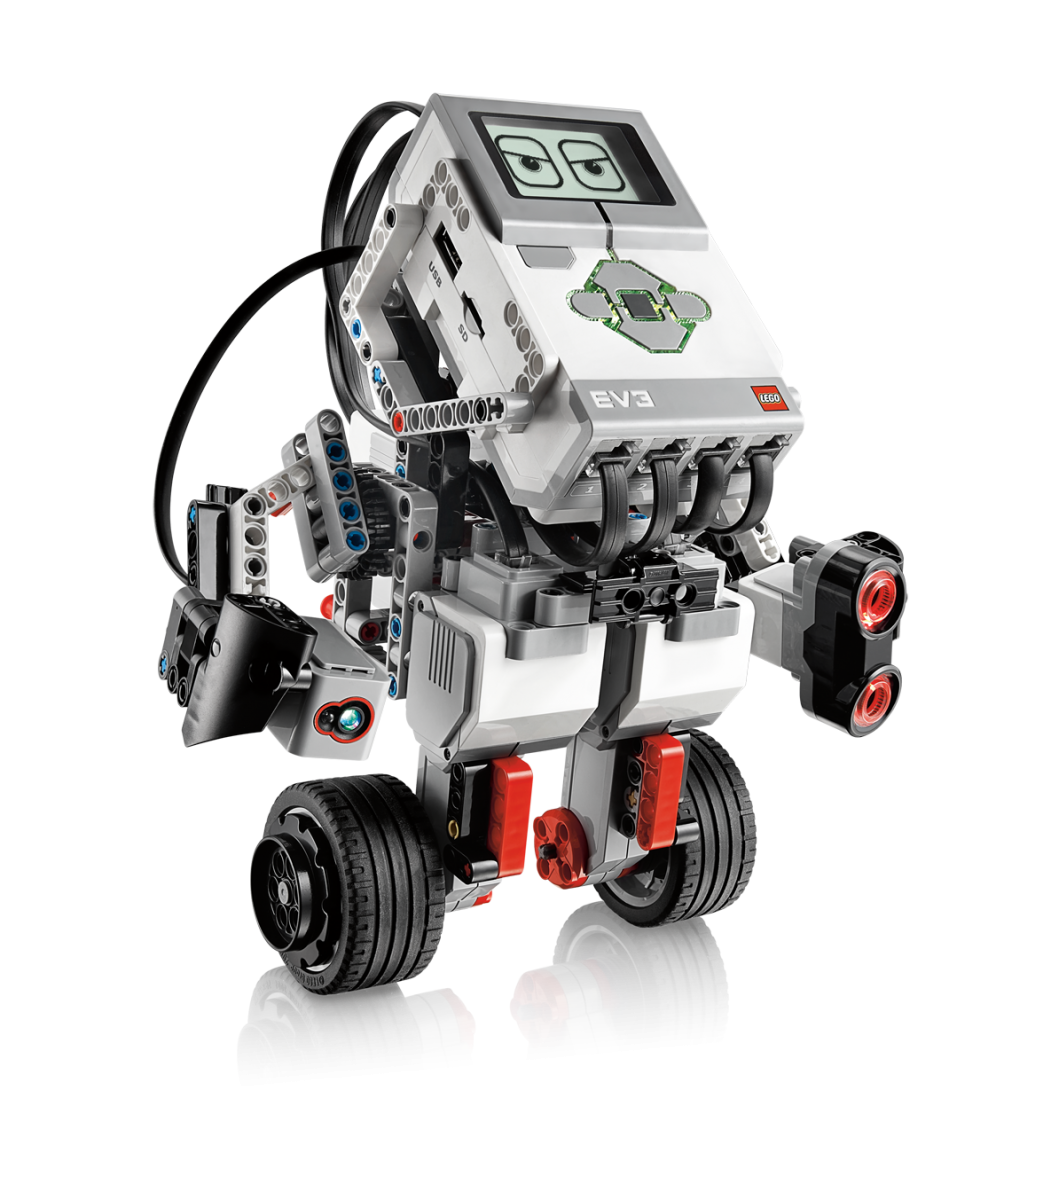
\includegraphics[width=250px]{images/lego-mindstorms-ev3_Robotics-for-Kids.png}
	\caption[\legoEV{ }-- samobalancující robot]{\legoEV{ }-- samobalancující robot\protect\footnotemark}
	\label{fig:lego-mindstorms-ev3_Robotics-for-Kids}
\end{figure}


\footnotetext{Zdroj: \url{https://www.bermotech.com/training/coding-for-teenagers-and-children/y-robotics-with-lego-mindstorm-ev3/}}

\begin{figure}[h]
	\centering
	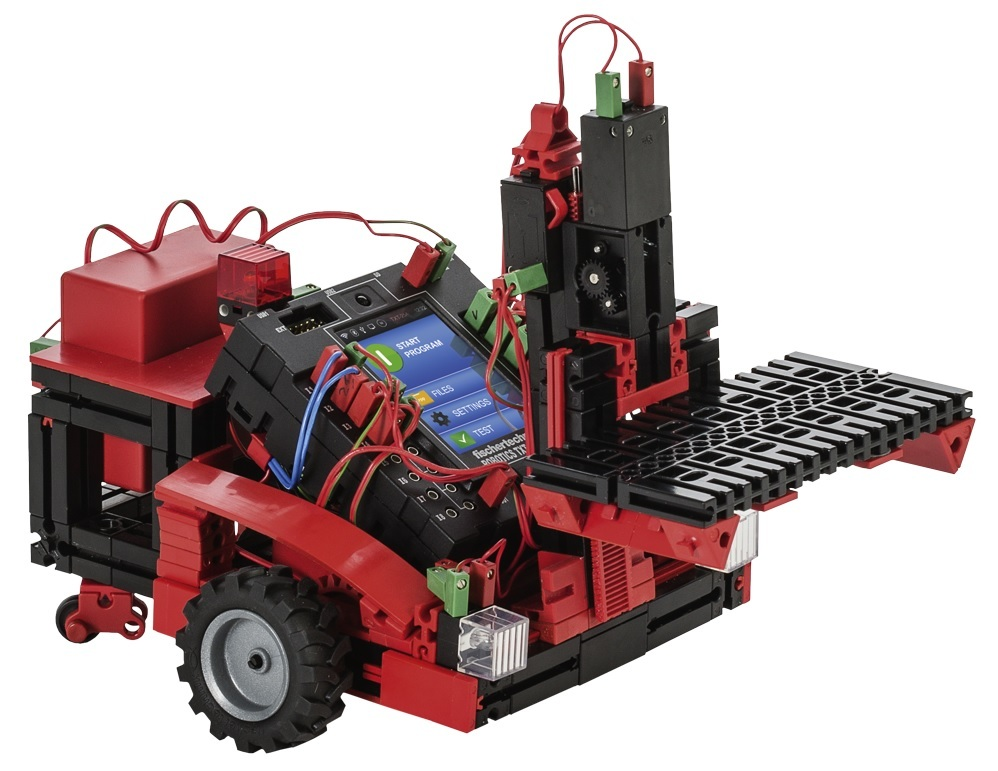
\includegraphics[width=250px]{images/fischertechnik_ROBO-TX-Explorer_02.jpg}
	\caption[Fischertechnik -- ROBO TX Explorer]{Fischertechnik -- ROBO TX Explorer\protect\footnotemark}
	\label{fig:fischertechnik_ROBO-TX-Explorer}
\end{figure}

\footnotetext{Zdroj: \url{http://www.helago-cz.cz/eshop-519143-workstation-robo-tx-training-lab-tx-explorer-146560.html}}

Existuje i mnoho podobných stavebnic~\cite{intorobotics_BestAlternativesToLegoMindstormsKits}. 
Například \fischerT prodává podobné robotické sety jako \lego{~}\cite{fischertechnik_ROBOTICS}. 

Uživateli nabízí rozsáhlejší pohled do elektroniky a~fungování jednotlivých modulů. 
Umožňuje také relativně snadno přidat vlastní moduly.
Zároveň má jednoduché grafické programovací prostředí podobně jako \lego. 
\FischerT{ }ovšem není tak rozšířen jako \legoM, protože ačkoliv nabízí v~některých ohledech více funkcí, zároveň klade větší nároky na uživatele, je podstatně dražší (základní set~\cite{fischertechnik_HelagoEshop_ROBOTICS-TXT-COMPETITION-SET} stojí cca dvakrát tolik co \legoEV{ Základní souprava}~\cite{lego_eduxeEshop_CoreSet}) a~nemá takový věhlas a~značku.

% figure + footnote -> minipage 
%src: http://www.tex.ac.uk/FAQ-ftncapt.html
% \begin{figure}[h]
% \begin{minipage}{\textwidth}
%  	\centering
% 	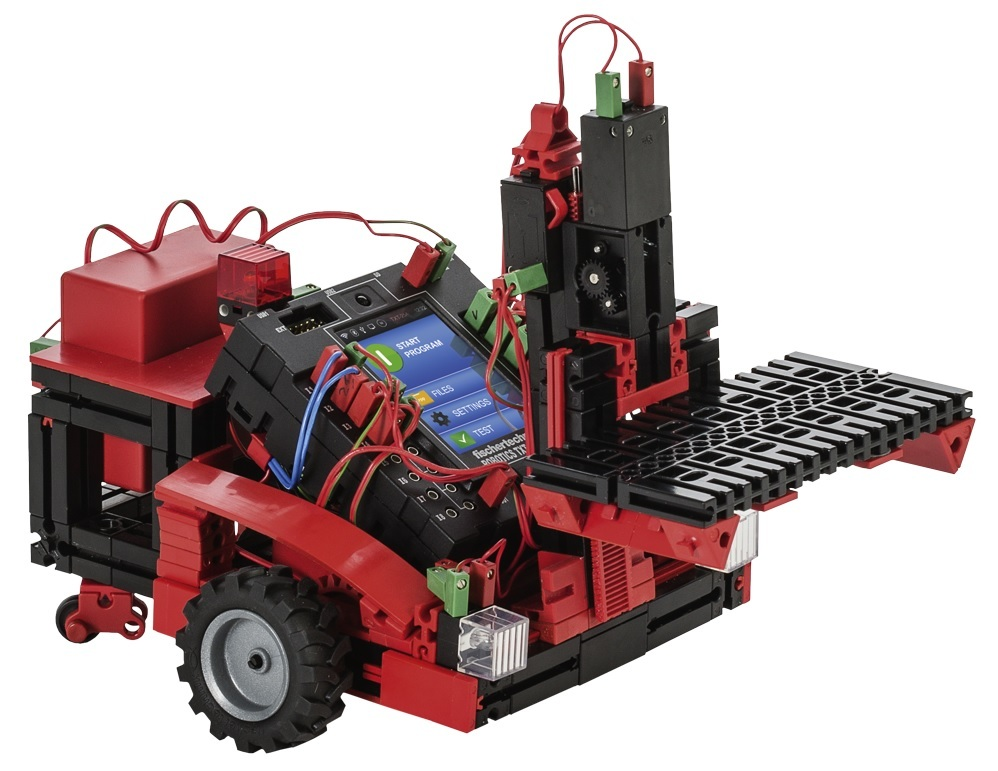
\includegraphics[width=300px]{images/fischertechnik_ROBO-TX-Explorer_02.jpg}
% 	\caption[Fischertechnik - ROBO TX Explorer]{Fischertechnik - ROBO TX Explorer \footnote{Zdroj: \url{http://www.helago-cz.cz/eshop-519143-workstation-robo-tx-training-lab-tx-explorer-146560.html}}
% \end{minipage}
% \end{figure}

% figure + footnote -> afterpage
% src: http://tex.stackexchange.com/questions/10181/using-footnote-in-a-figures-caption
%\afterpage{
%	\begin{figure}[h]
%	 	\centering
%		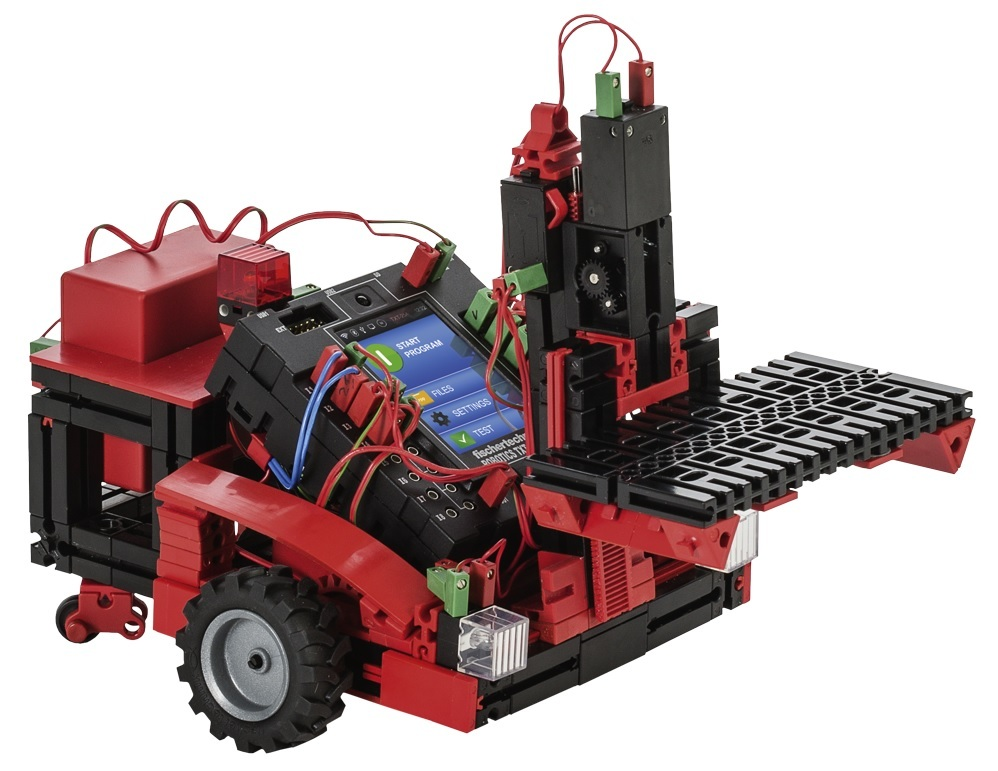
\includegraphics[width=300px]{images/fischertechnik_ROBO-TX-Explorer_02.jpg}
%			\caption[Fischertechnik - ROBO TX Explorer]{Fischertechnik - ROBO TX Explorer \footnotemark}
%		\label{fig:fischertechnik_ROBO-TX-Explorer}
%	\end{figure}
%	\footnotetext{Zdroj: \url{http://www.helago-cz.cz/eshop-519143-workstation-robo-tx-training-lab-tx-explorer-146560.html}}
%}

\begin{figure}[h]
	\centering
	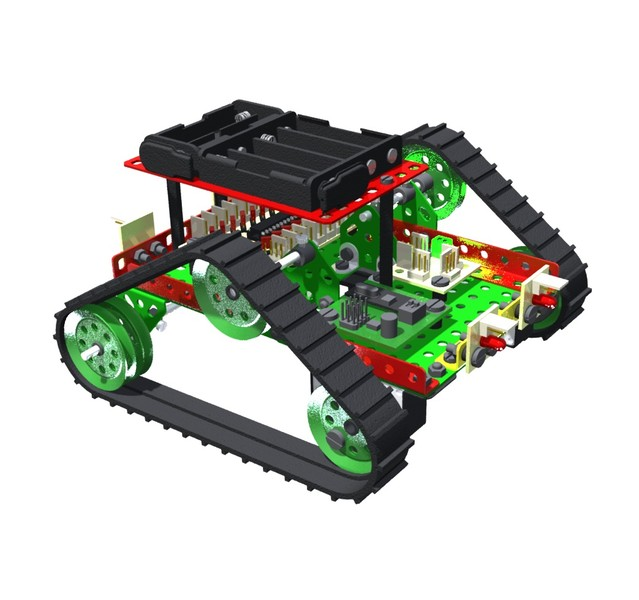
\includegraphics[width=235px]{images/MERKUR_Pasovy-podvozek-01_ATMEL+RC.jpg}
	\caption[MERKUR -- Pásový podvozek 01 -- ATMEL + RC]{MERKUR -- Pásový podvozek 01 -- ATMEL + RC\protect\footnotemark}
	\label{fig:MERKUR_Pasovy-podvozek-01_ATMEL+RC}
\end{figure}

\footnotetext{Zdroj: \url{http://www.merkurtoys.cz/vyrobky/pasovy-podvozek-merkur-s-elektronikou-rc}} 

Další zajímavou stavebnicí jsou Robotické sety od \merkur{u}~\cite{merkur_roboticsSetsEshop}. 
Nabídka jednotlivých setů je relativně široká a~v~porovnání s~\legoM{ }nebo \fischerT{ }nabízí ještě bližší kontakt s~elektronikou a~samotným hardwarem. 
Jako řídicí mikrokontroléry můžete využít PIC nebo megaAVR od firmy Microchip. 

Vzhledem k~použitým procesorům je možné tyto stroje programovat v~C/C++, PICAXE BASIC nebo i~v~grafickém prostředí~\cite{picaxeCz_BlocklyForPICAXE}. 
Robotické stavebnice od Merkuru mají podobné \uv{problémy} jako \fischerT. 
Kladou na uživatele větší nároky, nemají tak zvučnou značku, mají omezenější základní sadu senzorů a~neumožňují tak rychlou stavbu fungujícího robota.

Na závěr lze zmínit výukové roboty, kteří jsou primárně, na rozdíl od robotických stavebnic, zaměřeny na velmi úzkou oblast činností (jízda po čáře, plnění jednoduchých sekvenčních úkolů, \dots). 
Tyto roboty jsou zajímavé z~pohledu ceny, ale i~jednoduššího využití ve výuce (žáci nemusí sestavovat konstrukci a hardware je plně připraven k~používání). 

Naopak již neumožňují rozvoj kreativity studentů při stavbě a přizpůsobení robota pro různé soutěže (většinou je lze využívat jen v~jedné soutěžní kategorii).  
Mezi takovéto roboty patří například Pololu~3pi~\cite{robotPololu3pi} (primárně určen pro jízdu po čáře -- zvládá jezdit až~1~m/s) nebo Edison~\cite{robotEdison} (umí sledovat čáru, lze jej programovat graficky i~v~Pythonu, má různé senzory, je možné jej kombinovat s~\lego{ }kostkami). 

Tyto roboty ovšem neumožňují takový rozsah činností jako \legoM.

\begin{figure}[h]
	\begin{minipage}[b]{.5\textwidth}
		\centering
		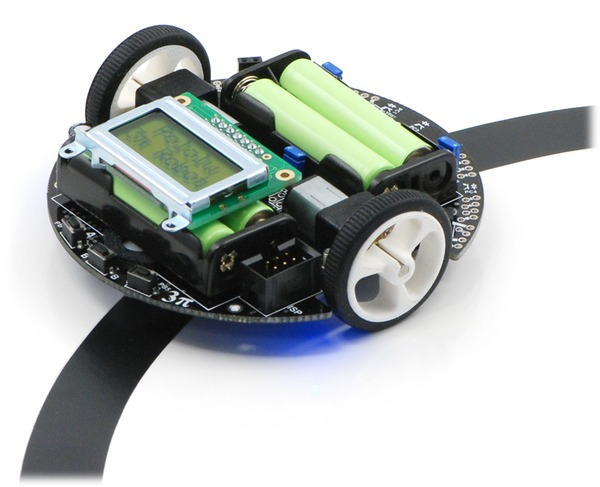
\includegraphics[width=\textwidth]{images/pololu-3pi-robot-8-on-line.jpg}
		\caption[Robot Pololu 3pi]{Robot Pololu 3pi\protect\footnotemark}
		\label{fig:pololu-3pi-robot-8-on-line}
	\end{minipage}
	\hfill
	\begin{minipage}[b]{.5\textwidth}
		\centering
		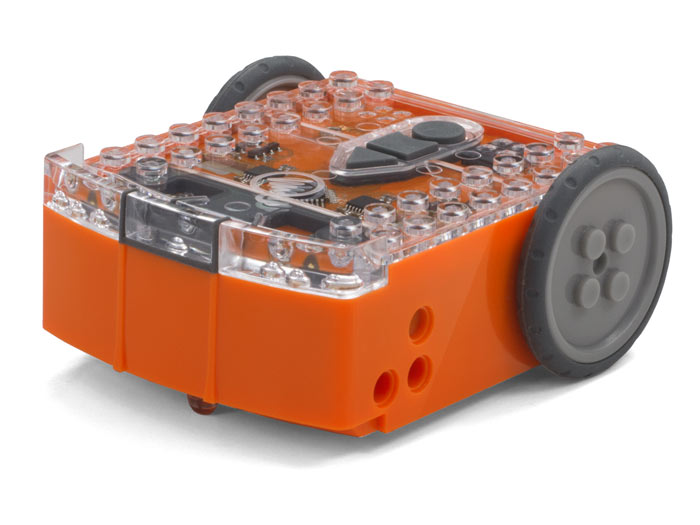
\includegraphics[width=\textwidth]{images/Edison-Educational-robot.jpg}
		\caption[Robot Edison]{Robot Edison\protect\footnotemark}
		\label{fig:Edison-Educational-robot}
	\end{minipage}
\end{figure}

% two footnote/footnotemark in minipage - problem with index
% solution: http://tex.stackexchange.com/a/43694

\addtocounter{footnote}{-1} % footnote_cnt -= 1
\footnotetext{Zdroj: \url{https://www.pololu.com/product/975}}
\stepcounter{footnote}
\footnotetext{Zdroj: \url{https://meetedison.com/meet-edison-v2-0/}}


% putting two images beside each other
% source: http://tex.stackexchange.com/a/148445

%\begin{figure}[!tbp]
%	\begin{subfigure}[b]{.5\textwidth}
%		\centering
%		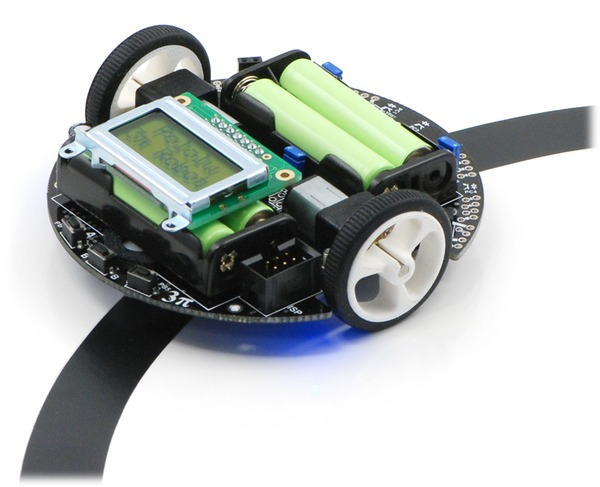
\includegraphics[width=\textwidth]{images/pololu-3pi-robot-8-on-line.jpg}
%		\caption[Robot Pololu 3pi]{Robot Pololu 3pi\protect\footnotemark}
%		\label{fig:pololu-3pi-robot-8-on-line}
%	\end{subfigure}
%	\hfill
%	\begin{subfigure}[b]{.5\textwidth}
%		\centering
%		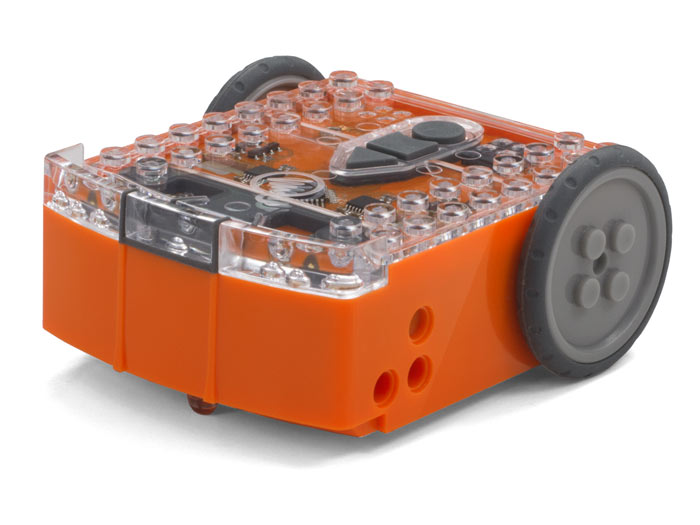
\includegraphics[width=\textwidth]{images/Edison-Educational-robot.jpg}
%		\caption[Robot Edison]{Robot Edison\protect\footnotemark}
%		\label{fig:Edison-Educational-robot}
%	\end{subfigure}
%	\caption{Roboti se zaměřením na velmi úzkou oblast činnost}
%\end{figure}
%
%\footnotetext{Zdroj: \url{https://www.pololu.com/product/975}} 
%\footnotetext{Zdroj: \url{https://meetedison.com/meet-edison-v2-0/}} 

\section{Motivace autora}

Již čtvrtým rokem vedu robotický kroužek na své bývalé střední škole SPŠ a VOŠ Brno, Sokolská a~zároveň organizuji tábory a~další vzdělávací akce v~oblasti techniky a~robotiky na pobočce Robotárna, Dům děti a~mládeže Brno, Helceletova.
Už na střední škole jsem se v~rámci těchto dvou organizací účastnil různých soutěží, jako například Robotický den v~Praze, Mikrokontroléry letí na FEKT VUT Brno nebo Středoškolská odborná činnost (obory strojírenství a~elektrotechnika). 
Z~některých soutěží jsem si dovezl cenná umístění, ale~i~mnoho zkušeností, inspirace a~podnětů na přemýšlení.


Za dobu, kterou se věnuji programování mikrokontrolérů a~robotice, jsem již narazil na mnoho překážek a~problémů, které bylo třeba překonat. 
%si už mnohokrát prošel trnitou cestou 
Tyto překážky jsou ovšem výrazně náročnější pro studenty, kteří v~těchto oblastech teprve začínají a~seznamují se s~nimi. 

Často může nastat i~situace, kdy je student se zájmem o~robotiku odrazen její počáteční složitostí.

Přitom by z~něj mohl být v~budoucnu perfektní programátor. 
Jen mu zrovna tenhle mikrokontrolér nejde naprogramovat nebo mu koupený H-můstek nechce roztočit motor.

Proto se svým studentům vždy snažím nachystat co nejlepší prostředí pro začátky s~robotikou. 

Již jsem zkoušel různé platformy (například využít k~výuce robota Pololu~3pi) i~způsoby výuky (kombinace elektroniky, programování na PC a~programování mikrokontrolérů), ale~bohužel vždy jsem se dostal do stejné situace. 

Ačkoliv mi studenti chodili již rok do robotického kroužku, pořád je dělily minimálně dva roky od schopnosti postavit a~naprogramovat složitějšího robota (s~tím, že by použili předpřipravenou elektroniku, ale rozuměli tomu, co je jak zapojeno + uměli použít dostupné knihovny a~naprogramovat si chování svého robota).

Nedávno jsme ale do kroužku zakoupili \legoEV{}. 
Stavebnici, která mi měla umožnit postavit robota za den. 
Prakticky stavebnice snů. No není to nádherná představa?
A~opravdu tomu tak bylo. Robota jezdícího po čáře jsme s~manuálem zvládli poskládat a~zprovoznit za den. 
Studenti nemuseli studovat a~řešit zapojení jednotlivých komponentů do řídicí elektroniky. 

Nebylo třeba trávit mnoho času vysvětlováním způsobu programování 8bitových mikrokontrolérů (omezení paměti a~výkonu, menší datové typy -- \verb|uint_8t|, komunikace po sériové lince, \dots).

Jen si poskládali z~\lega{ }hardware, pomocí kabelů (které nelze otočit ani zapojit špatně a~tím něco zničit) spojili jednotlivé moduly. 

A~v~grafickém prostředí si poskládali svůj program.

Pak jsme se ale začali soustředit na zlepšování softwaru i~hardwaru tak, abychom využili stavebnici na 100~procent, a~v~ten moment jsme narazili.

Dokud jsme si s~EV3 jen \uv{hráli} a~nesoustředili se primárně na výkon a~spolehlivost, bylo vše v~pořádku. 
Jakmile jsme ale chtěli mít regulační smyčku PID~regulace pro robota na sledování černé čáry s~periodou 10~ms, zjistili jsme, že to nejde (a~to máme v~EV3 \brick{\it u} 300~MHz~ARM). Přitom díky předešlým zkušenostem s~8bitovými mikrokontroléry Atmel~AVR jsme věděli, že by to neměl být problém.


To samé platí o~grafickém vývojovém prostředí dodávaném s~\EVthree. Dokud máte na obrazovce několik programových bloků, vše funguje bez problémů. 
Když se však program rozroste na několik obrazovek a~samostatných modulů, velmi rychle ztrácíte přehlednost a~efektivitu programování.
Zároveň vám již moc nepomohou ladicí nástroje, které jsou součástí prostředí, protože při jednoduchém programu je lze relativně dobře využít, ale při rozsáhlejších programech již nejsou k~dispozici nebo je jejich použití velmi komplikované. 


Proto jsme začali hledat alternativní platformy, které by odstraňovaly zmíněné problémy, což vyústilo v~tuto práci.   


  
  \chapter{Historie \legoM}

Historie firmy \lego{ }je velmi dlouhá a~sahá až do roku 1932~\cite{lego_GroupHistory1930s}. 
V období, kdy se počítače stávají standardní součástí domácnosti, se dostávají í do \lego{} a tím roku 1998 vzniká  \legoM{}~\cite{lego_mindstormsHistory}.
% * <kuba.streit@gmail.com> 2017-05-07T14:53:32.539Z:
% 
% Postupně čtu a myslím si:
% LEGO 1932 - super, Mindstorms prakticky to samé? Zajímavé, to bych nečekal. To samé = 1998 - what?
% Spíš bych to asi zkusil přeformulovat tak nějak, jako že v období, kdy se počítače stávají standardní součástí domácnosti, dostávají se i do Lega a tím vzniká Mindstorms.
% 
% ^ <paral.jarek@gmail.com> 2017-05-07T19:10:12.410Z:
%
% Předělám.
%
% ^ <paral.jarek@gmail.com> 2017-05-07T21:57:01.485Z:
%
% Hotovo.
%
% ^.

% TODO: kapitola LEGO TECHNIC

\section{\legoM{ }RCX}

První verze byla označena jako \legoM{ }RCX\footnote{RCX = Robotic Command eXplorers} Intelligent Brick and Robotics Invention System a~obsahovala 8bitový mikrokontrolér Hitachi H8/3292~\cite{hitachi_microcontrolerH8series} s~procesorem H8/300 taktovaným na 16~MHz a~s~32~KB~RAM~\cite{legoMindstormsRCX_Manual}.

\begin{figure}[h]
	\centering
	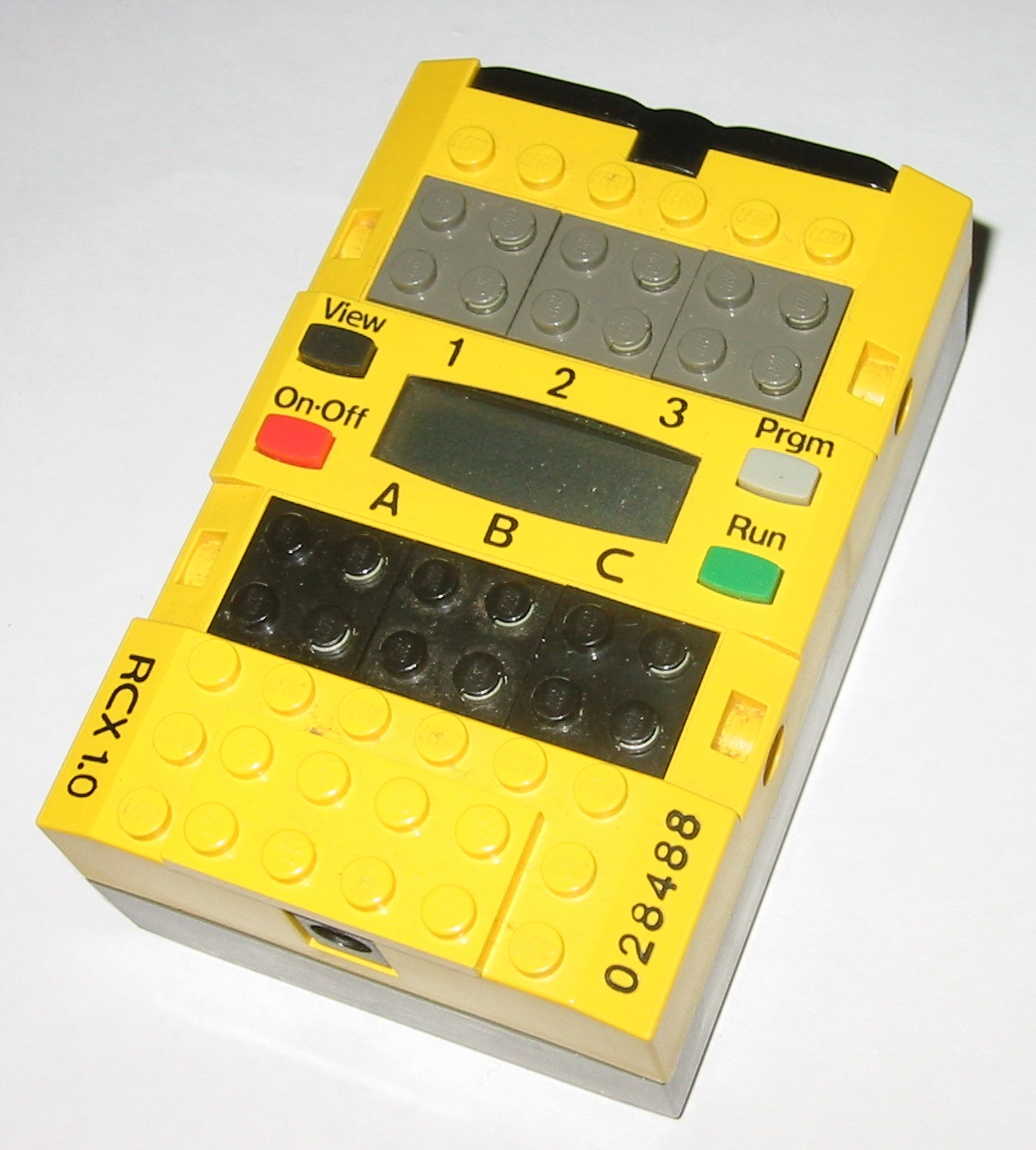
\includegraphics[width=250px]{images/lego-mindstorms-rcx_wikipedia.jpg}
	\caption[\legoM{ }RCX]{\legoM{ }RCX\protect\footnotemark}
	\label{fig:lego-mindstorms-rcx-wikipedia}
\end{figure}

\footnotetext{Zdroj: \url{https://en.wikipedia.org/wiki/Lego_Mindstorms}} 

Oficiálně bylo možné stavebnici programovat ve dvou prostředích. První prostředí ROBOLAB, založené na programu \labview{ }od firmy \NI, bylo pro výukové účely (do škol) a~bylo součástí výukového setu. 
Běžní zákazníci (lidé, kteří si kupovali stavebnici domů) měli k~dispozici RCX Code, které bylo jednodušší na obsluhu a používání, ale nemělo tak rozsáhlé možnosti programování. 
Zároveň vznikla i~vývojová prostředí třetích stran, která umožňovala programování v~mnoha běžně používaných jazycích (C++, Java,~\dots).

Již v~prvním roce prodeje stavebnice vznikla soutěž {\it FIRST} LEGO League (FLL)\footnote{{\it FIRST} = For Inspiration and Recognition of Science and Technology}. 
Cílem soutěže je povzbudit a~motivovat k~navrhování, stavění a`programování vlastních inteligentních systémů~\cite{lego_FLL-about}. 
Jednotlivá kola probíhají po celém světě a~lze postoupit až do celosvětového finále. % TODO: FLL - ověřit možnost postupu do celosvětového finále
Účastníci musí být ve věku od 10 do 16 let. 

\section{\legoM{ }NXT}

Následující verzi vydalo \lego{ }v roce 2006~\cite{lego_mindstormsHistory}. 
Byl kompletně změněn způsob připojování jednotlivých modulů. 
Moduly se již nepřipojují pomocí speciálních \lego{ }kostek, ale využívají upravený konektor RJ-12 % TODO: upravený konektor -> méně běžnou variantu konektoru RJ-12
(kolík sloužící pro správné zapojení konektoru je oproti běžné telefonní RJ-12 umístěn mimo střed~\cite{legoMindstorms_rj12-connector}). % -- na pravou stranu z pohledu od kabelu 

\begin{figure}[h]
	\centering
	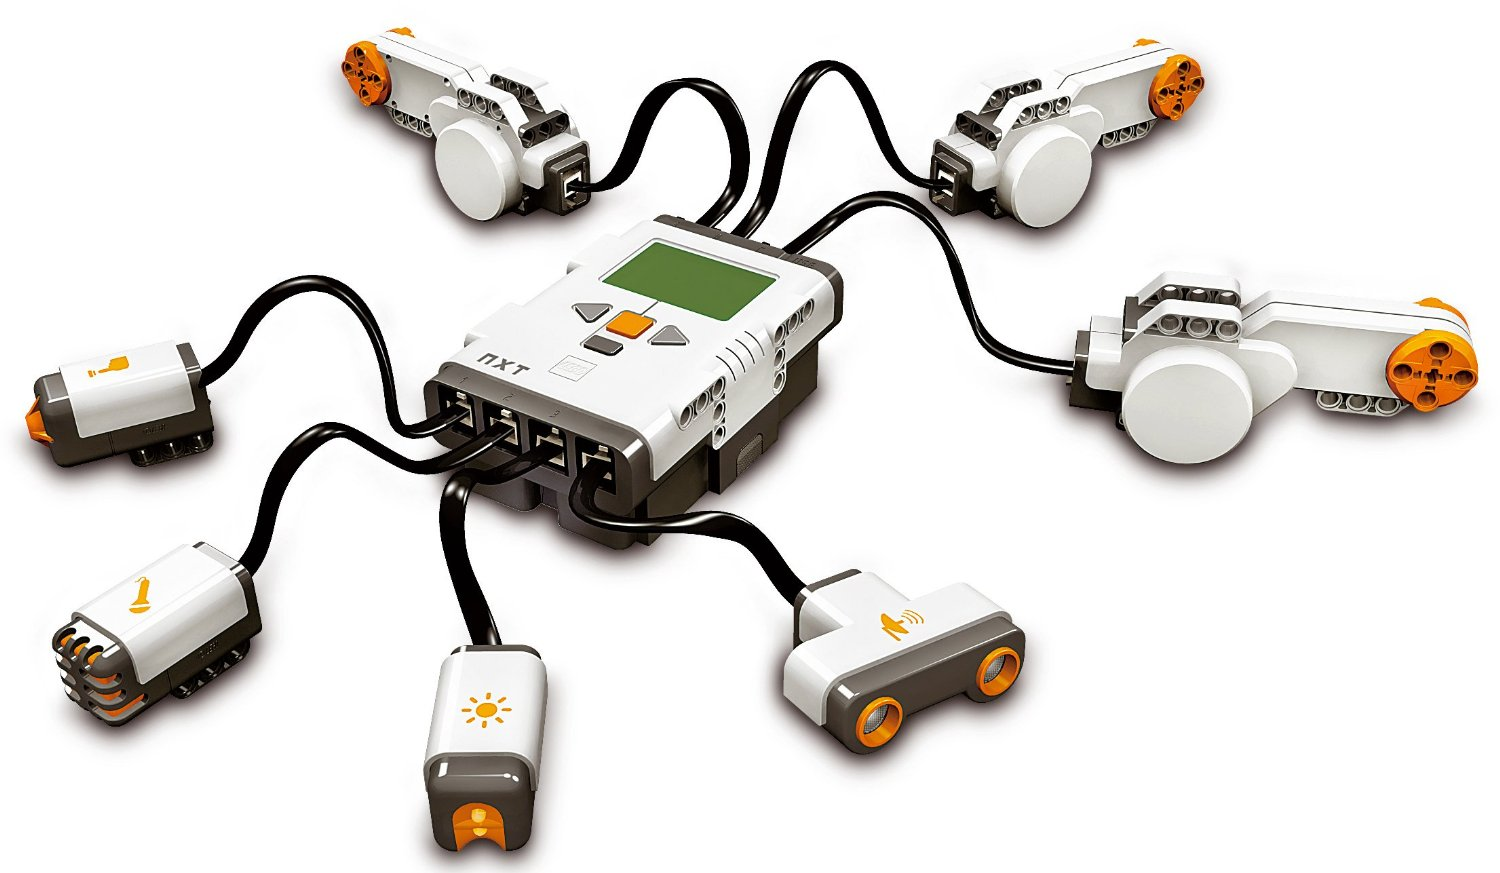
\includegraphics[width=\textwidth]{images/lego-mindstorms-nxt_with-modules.jpg}
	\caption[\legoNXT{ }s komponenty, které lze používat]{\legoNXT{ }s komponenty, které lze používat\protect\footnotemark}
	\label{fig:lego-mindstorms-nxt_with-modules}
\end{figure}

Řídicí kostka (dále jen \brick{}) % TODO: formátování speciálních výrazů

se již neprogramuje přes infraport, ale využívá se standardní USB kabel, případně integrovaný Bluetooth~\cite{legoMindstormsNXT_hardware}.

Po hardwarové stránce došlo ke značnému posunu. Původní 8bitový mikrokontrolér byl nahrazen 32bitovým ARM mikrokontrolérem % TODO: mikrokontrolér/mikroprocesor/procesor

AT91SAM7S256 (256~KB~FLASH, 64~KB~RAM, 48~MHz) a~k~němu byl přidán 8bitový ko-procesor ATmega48 (4~KB~FLASH, 512~Byte~RAM, 8~MHz). 
Oba tyto procesory dodávala firma Atmel (nyní již Microchip)~\cite{legoMindstormsNXT_hardware}.

\footnotetext{Zdroj: \url{http://www.itnetwork.cz/java/lego-nxt/seznameni-s-nxj-pro-lego-nxt}} 

\brick{ }lze programovat pomocí vývojového prostředí NXT-G\footnote{NXT-G = NXT Graphic - grafické} (viz obrázek \ref{fig:lego-mindstorms-nxt-g}), které \lego{ }vyvinulo opět ve spolupráci s~\NI{~}\cite{legoMindstormsNXT_NXT-G}. 
Zároveň \NI{ }dodává toolbox do \labview{}, ve kterém lze \brick{ }také programovat. 

\legoNXT{ }má ovšem bohatou nabídku alternativních programovacích prostředí, která lze využít k~vytváření kódu pro \brick. 
Některá fungovala již na RCX a~byla upravena i~pro NXT. 
Jako příklad mohu uvést jedno z~nejpoužívanějších prostředí BricxCC\footnote{BricxCC = Bricx Command Center} s~jazykem NXC\footnote{NCX = Not eXactly C}. 
NCX je vysokoúrovňový open-source jazyk podobný C~\cite{legoWikipediaNXT_NXC}.

\begin{figure}[h]
	\centering
	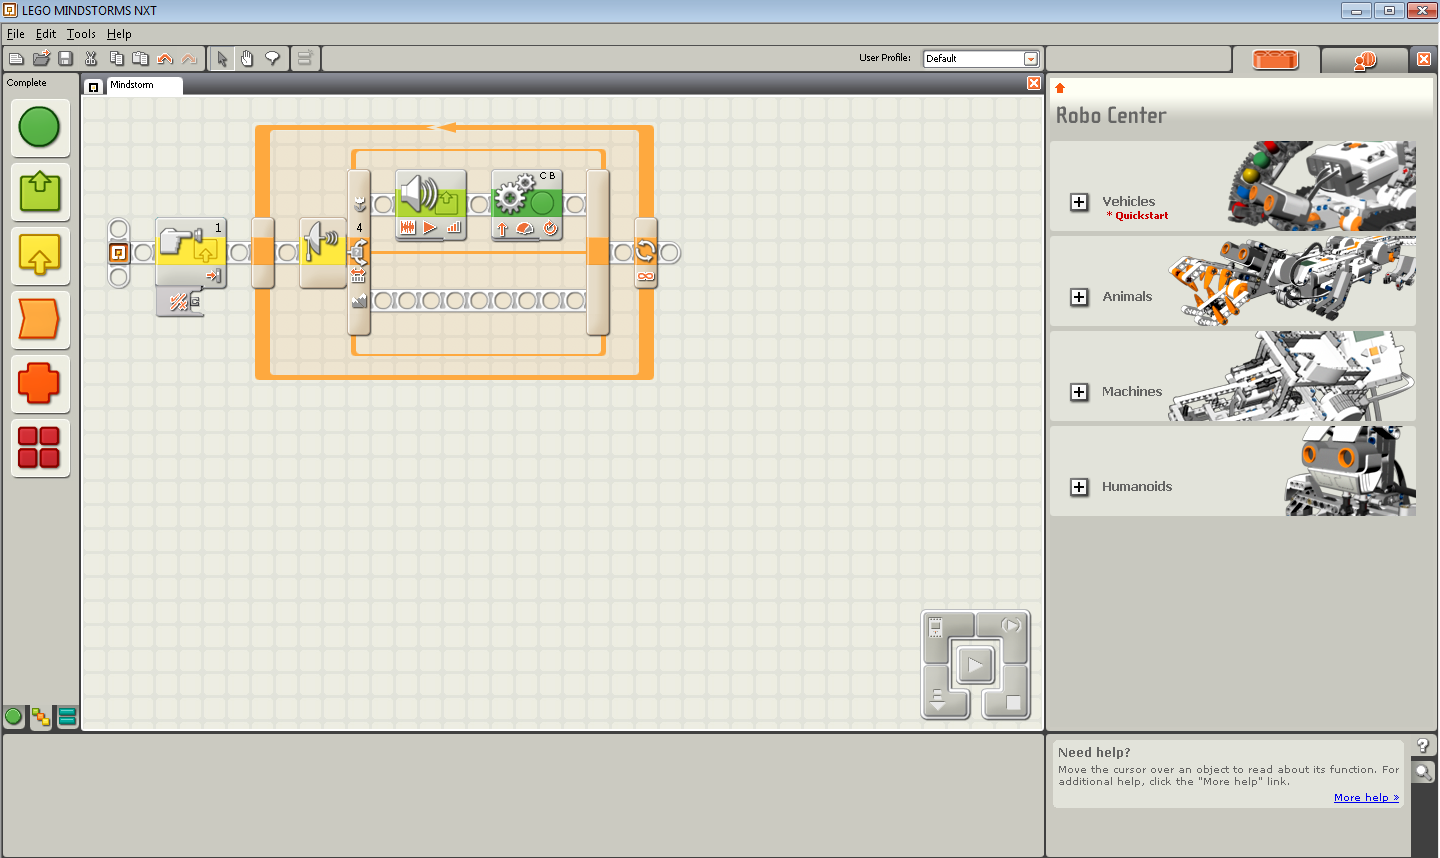
\includegraphics[width=\textwidth]{images/lego-mindstorms-nxt-g.png}
	\caption[\legoNXT{-G}]{\legoNXT{-G}\protect\footnotemark}
	\label{fig:lego-mindstorms-nxt-g}
\end{figure}

\footnotetext{Zdroj: \url{http://lukedainton-robots.blogspot.cz/2012/07/control-systems-shooterbot-nxt-g.html}} 
Existují ale i~komerční varianty. 
Například ROBOTC~\cite{legoProgramingPlatform_ROBOTC} je univerzální programovací prostředí a~jazyk umožňující programovat větší množství hardwaru (od \legoM{ }RCX, NXT, EV3 až po Arduino nebo PIC). 
Jak již název napovídá, ROBOTC je založen na jazyku C (ANSI-C).
Uživatel ovšem může přecházet mezi grafickou a~textovou formou programování, což může být pro začátečníky velmi vhodné.
Také má možnost vybrat si úroveň abstrakce, na jaké bude v~textovém módu pracovat.  

ROBOTC je velmi zajímavé prostředí. Bohužel nikdy nebyla vydána objektová varianta, s~kterou by mohlo být programování ještě jednodušší. 
Zároveň se jedná o~placený produkt a~jednotlivé licence~\cite{legoProgramingPlatform_ROBOTC-price} tvoří přibližně čtvrtinu současné ceny základní sady stavebnice \legoEV{~}\cite{lego_eduxeEshop_CoreSet}, což už není nezanedbatelná částka.

Pro NXT existuje celá řada dalších platforem a~jazyků (Javy, C\#, Lua, Ada, Python~\cite{legoMindstormsNXT_Programming}), které lze použít. 
Jelikož je ale tato práce zaměřena na \legoEV{ }, nebudou tyto platformy dále řešeny. 

\section{\legoM{ }EV3}

Aktuálně nejnovější verzí stavebnice \legoM{ }je verze EV3, která byla vydána v~roce 2013~\cite{lego_mindstormsHistory}. 
Proběhlo u~ní mnoho inovací a~změn, i~tak ale byla zachována velmi dobrá kompatibilita s~verzí NXT~\cite{legoRobotSquare_EV3-and-NXT-compatibility}.

EV3 přináší zásadní změnu procesoru. 
Jedná se o~32-bitový~ARM (ARM9), tentokrát ale od firmy Texas Instrument, s~označením AM1808 (16~MB~FLASH, 64~MB~RAM, 300~MHz)~\cite{legoMindstormsEV3_fw-dev-kit}. 
Kvůli správě paměti již musí tento procesor používat operační systém. % TODO: doplnit info o správě paměti na ARM9 
\lego{ }pro EV3 vytvořilo upravenou verzi Linuxu. 

\begin{figure}[h]
	\centering
	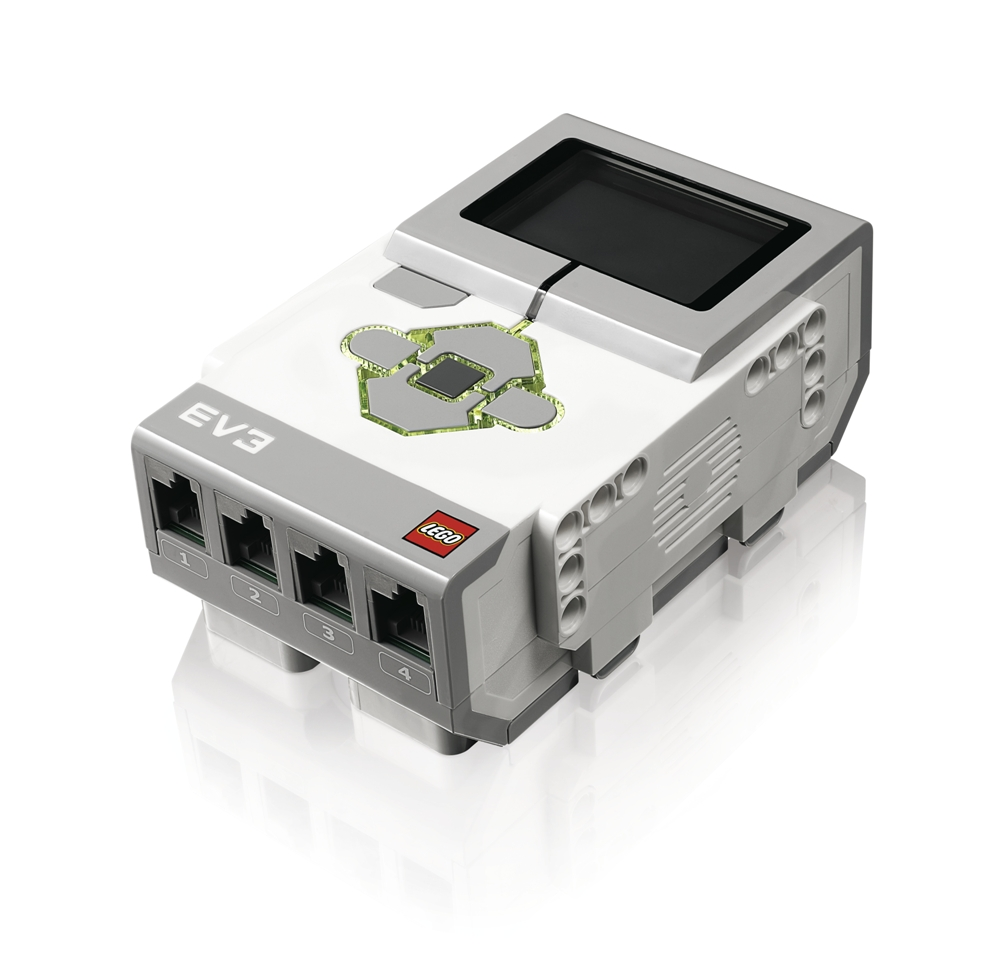
\includegraphics[width=330px]{images/lego-mindstorms-ev3_brick.jpg}
	\caption[\legoEV{ Brick}]{\legoEV{ \brick}\protect\footnotemark}
	\label{fig:lego-mindstorms-ev3_brick}
\end{figure}

\footnotetext{Zdroj: \url{http://hackeducation.com/2015/04/10/mindstorms}} 

Nová verze obsahuje také čtečku Micro SD karet, USB host interface a~jeden výstupní port pro motory navíc (celkem 4~porty, NXT jen 3~porty) \cite{legoBotBench_comparing-EV3-and-NXT}. 

Slot na SD karty umožňuje rozšířit paměť pro programy, ale lze jej hlavně využít pro spouštění alternativních operačních systémů. 

Díky USB host interface lze k~EV3 připojovat různé periferie, pro které je v~systému a~vývojovém prostředí připravená obsluha.
Lze tak připojit Wifi modul nebo klávesnici. 
% * <kuba.streit@gmail.com> 2017-05-07T15:03:27.550Z:
% 
% Musí to umět systém, vývojové prostředí bych tu nezmiňoval. 
% Navíc z toho, co jsme zkoušeli, jediný prostředí, který umí víc než Wifi, je ev3dev.
% 
% ^ <paral.jarek@gmail.com> 2017-05-07T18:50:35.270Z:
%
% JJ to musím přeformulovat:  "Díky USB host interface lze k~EV3 připojovat různé periferie, pro které je v~systému a~vývojovém prostředí připravená obsluha.
% Lze tak připojit Wifi modul, klávesnici nebo myš. "
%
% ^ <paral.jarek@gmail.com> 2017-05-08T13:29:14.648Z:
%
% Ponecháno.
%
% ^.
Zároveň můžete přes USB kabel spojit až čtyři EV3 \brick{\it y} a~ovládat je jedním programem (z~jednoho hlavního \brick{\it u}).

\begin{figure}[h]
	\centering
	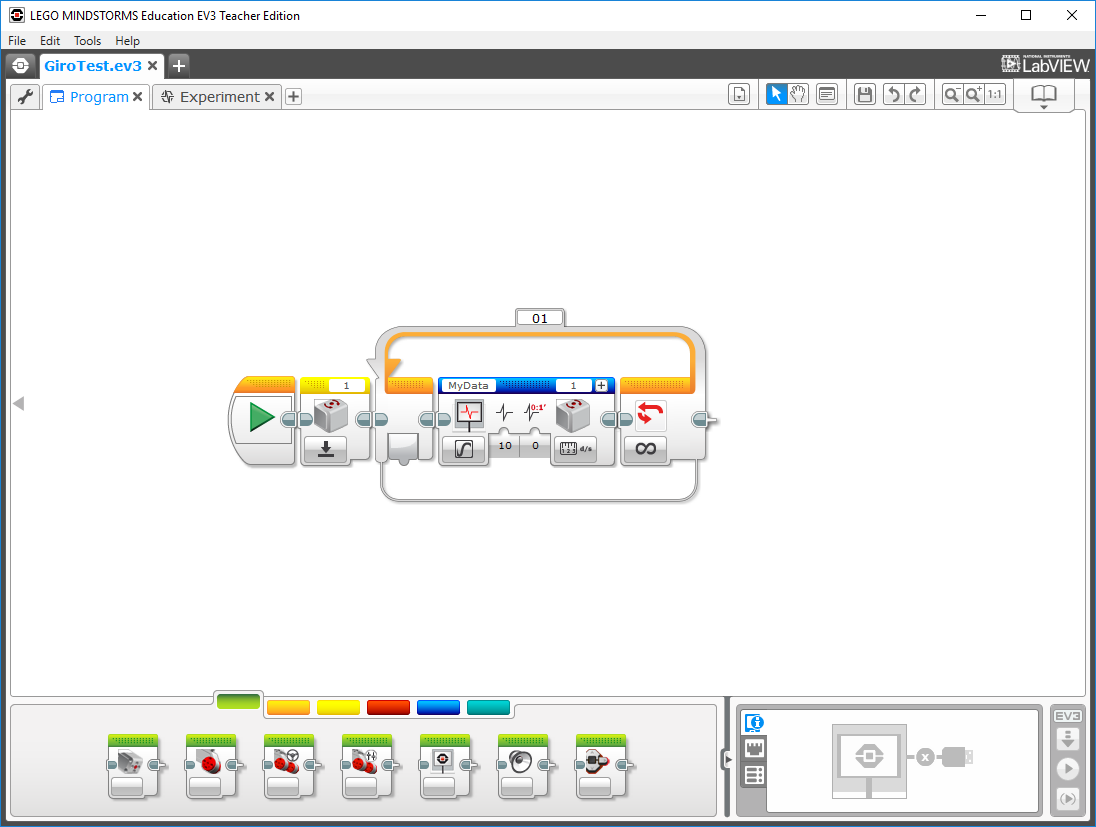
\includegraphics[width=\textwidth]{images/lego-mindstorms-ev3_dev-soft.png}
	\caption[\legoM{ }Education EV3 Software -- vývojové prostředí]{\legoM{ }Education EV3 Software -- vývojové prostředí}
	\label{fig:lego-mindstorms-ev3_dev-soft}
\end{figure}

Programovací prostředí pro EV3 je znovu postaveno na \labview{ }a~ačkoliv se design v~porovnání s~prostředím pro NXT výrazně změnil (můžete porovnat obrázky \ref{fig:lego-mindstorms-nxt-g} a~\ref{fig:lego-mindstorms-ev3_dev-soft}), neměli by mít uživatelé NXT s~přechodem problém. 
Nové prostředí zvládne naprogramovat jak EV3, tak NXT \brick{}.

V~rámci alternativních platforem máme opět velký výběr \cite{legoMindstormsWikipedia_programming-languages}. 
Vhledem k~nutnosti používání operačního systému je většinou pro dané prostředí potřeba nahrát konkrétní systém na SD kartu a spustit \brick{ }s~touto kartou.

Jednotlivé alternativní platformy budou podrobněji probrány v~následující kapitole.

  
  \chapter{Dostupné platformy}

\label{lego-soft-available-platforms}


Pro \legoEV{} existuje mnoho vývojových platforem. 
Většinou se jedná o~specificky navržené programovací API ve~spojení s~vývojovým prostředím. 
Tyto platformy často fungují ve~spolupráci s~oficiálním systémem v~\EVthree{}, ale jsou i~platformy s~vlastním operačním systémem. 
V~tomto textu bude popsán jen výběr těch nejzajímavějších. % platforem. 

\section{Originální prostředí od \lego}

V~rámci této podkapitoly je rozebírán samotný operační systém na \EVthree{} a~také vývojové prostředí, určené pro tvorbu a~ladění programů. 
\lego{} si pro \EVthree{} vytvořilo vlastní operační systém, postavený na linuxovém jádru \cite{legoMindstormsEV3_fw-dev-kit}. 
Uvnitř systému běží virtuální stroj, který zpracovává byte-code uživatelské aplikace. 
Byte-code je vytvořen ve~vývojovém prostředí na PC a~pak je do \brick{\it u} odeslán po USB kabelu, Bluetooth nebo WiFi.

Celý systém s~vývojářskými nástroji a~dokumentací je volně k~dispozici na~webu~\cite{legoMindstorms_download}. Jelikož~\lego{} uvolnilo zdrojové kódy, mohly vzniknout alternativní systémy pro~\EVthree{} jako~\evThreeDev{} (kapitola~\ref{lego-ev3dev}) nebo \evRT{} (kapitola~\ref{lego-EV3RT}). 

\subsection{\legoSW{}}
\label{lego-soft-orig-problems}


\begin{figure}[h]
	\centering
	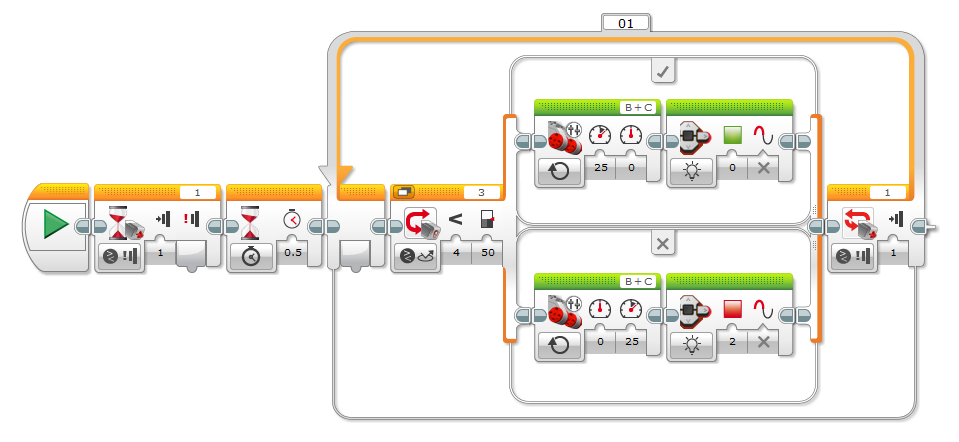
\includegraphics[width=0.99\textwidth]{images/lego-soft_robotut_switch-touch+motors+leds.png}
	\caption{Ukázka programovacích bloků v~\legoSW}
	\label{fig:lego-soft_example-blocks}
\end{figure}

\legoSW{} je~vývojářský program, který je k~\EVthree{} dostupný zdarma. 
Tento  software vytvořilo \lego{} ve~spolupráci s~firmou \NI{}. 
Je~tudíž postavený na~vývojovém prostředí \labview{}. 
\lego{} s~\NI{} již~spolupracovalo na předešlých vývojových prostředích. 
Program se~snaží působit jako profesionální vývojové a~laboratorní studio, což se~mu celkem daří.
Nabízí celou řadu funkcí od modulu pro programování přes tvorbu různých experimentů až~po přípravy interaktivních návodů a~průvodců programováním v~tomto prostředí.

V~režimu tvorby programu jsou hlavními stavebními kameny \EVblocks, které se ve~formě diagramů skládají do podoby výsledného programu (obrázek \ref{fig:lego-soft_example-blocks}).
Bloky jsou rozděleny do~několika skupin (akční, tok programu, senzory, datové operace, pokročilé a~vlastní), které se liší svojí barvou a~použitím. 
Pomocí těchto bloků lze řídit tok programu (podmínky, cykly, čekání a~vlákna), pracovat s~proměnnými, obsluhovat motory či senzory, provádět matematické operace anebo i~využívat vlastní bloky.

\begin{figure}[h]
	\centering
	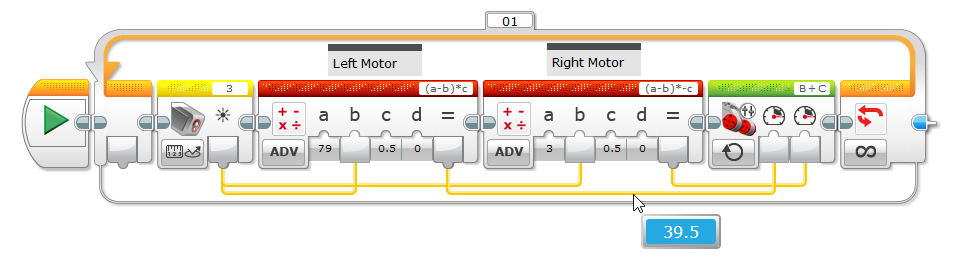
\includegraphics[width=\textwidth]{images/lego-soft_live-debugging_line-advance.png}
	\caption{Ukázka debuggování za běhu programu}
	\label{fig:lego-soft_live-debugging_line-advance}
\end{figure}

Vše je pěkně graficky zpracováno a~působí jako jednotný celek. 
Při běhu programu lze~sledovat jeho tok (kde v~diagramu se program nachází) nebo si třeba zobrazit aktuální stav (hodnotu proměnné, výsledek matematické operace, vstupní data ze~senzoru, \dots). 
Ukázku debuggování si~lze prohlédnout na obrázku \ref{fig:lego-soft_live-debugging_line-advance}, kde je vidět hodnota 39.5, odpovídající výsledku výpočtu výkonu pro levý motor v~závislosti na~naměřené hodnotě od barevného senzoru.
Zároveň je podle šrafování vrchní lišty bloků vidět, že~program aktuálně probíhá v~daném cyklu.

Pro práci s~\brick{\it em} je k~dispozici modul {\it Správa hardwaru}, kde si lze zjistit informace jako jméno, stav baterie, verze firmwaru nebo obsazenost paměti. 
Umožňuje také jednoduše nahrávat, spouštět a~ukončovat programy. 

Nalezneme zde i~správu připojení, v~rámci které lze vyhledávat a~připojovat se k~dostupným \brick{\it ům}. 
K~dispozici jsou tři druhy připojení: USB kabel, Bluetooth a~WiFi. Bluetooth je již integrován, ale pro použití WiFi je potřeba připojit WiFi modul.

\begin{figure}[h]
	\begin{minipage}[b]{.48\textwidth}
		\centering
		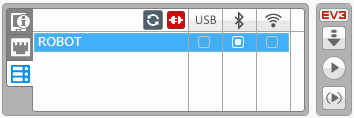
\includegraphics[width=\textwidth]{images/lego-soft_brick-manager_connected.png}
		\caption{Správa připojení k~\brick{\it u}}
		\label{fig:lego-soft_brick-manager-connected}
	\end{minipage}
	\hfill
	\begin{minipage}[b]{.48\textwidth}
		\centering
		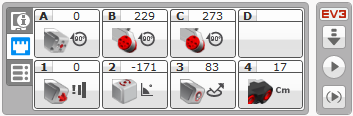
\includegraphics[width=\textwidth]{images/lego-soft_brick_port-view.png}
		\caption{Informační panel s~porty}
		\label{fig:lego-soft_brick_port-view}
	\end{minipage}
\end{figure}

Nejzajímavějším panelem je správce portů (obrázek~\ref{fig:lego-soft_brick_port-view}). 
Zobrazuje, na jakém portu je připojen který senzor nebo motor. 
Uživatel může vidět také aktuální hodnoty komponentů a~přepínat jejich režimy.    
Například u~barevného senzoru si~může vybrat, zda se bude zobrazovat barva, nebo odrazivost povrchu. U~motorů lze naopak nastavit, jestli má být ujetá vzdálenost zobrazování v~otáčkách, nebo ve~stupních. 
Tento panel považuji ze jednu z~nejpodstatnějších funkcí celého programu, jelikož dává uživateli dobrý přehled o~aktuálním stavu hardwaru. 
Jednoduše lze tak ladit konstanty v~programech (rozhodovací úroveň pro barevný senzor při detekci čáry, počet otáček motoru potřebných k~dojetí na~požadovanou pozici nebo vzdálenost od~překážky naměřenou ultrazvukem). 

V~následujících odrážkách je shrnut výčet nevýhod a~nedostatků originálního LEGO prostředí. 
Za nejdůležitější bod bych považoval nepřehlednost rozsáhlejších programů. % a nemožnost ladění a úpravy uživatelských bloků. 


To je pravděpodobně hlavní důvod, proč uživatelé \legoM{} vyhledávají alternativní prostředí. 
Ukázku rozsáhlejších programů je možné vidět na~obrázcích \ref{fig:lego-soft_legolib_converge_array}~a~\ref{fig:lego-soft_legolib_match_array_length}.\\

Nevýhody \legoSW:

\renewcommand{\labelitemi}{$-$} % nastavení pomlček místo plných koleček
\begin{itemize}[noitemsep]\itemsep2pt
	\item náročný na hardware počítače
	\item ve větších programech je obtížné se zorientovat anebo najít chybu
	\item nelze editovat proměnné ani rozhraní uživatelských bloků (jejich parametry)
	\item debuggovací režim nefunguje uvnitř uživatelských bloků
	\item při rozsáhlejších programech přestává prostředí fungovat (zamrzá a~padá)
	\item není dostupný na Linuxu a~není open-source
\end{itemize}

Nevýhody operačního systému v~\brick{\it u}:
\begin{itemize}[noitemsep]\itemsep2pt
	\item dlouhé zapínání a~vypínání
	\item značně pomalé zpracovávání některých operací (\dots) % TODO: dopsat operace
	\item nepracuje v~real-time režimu a~časování jednotlivých operací tedy není garantováno
	\item podpora jen jednoho typu WiFi modulu
\end{itemize}
\renewcommand{\labelitemi}{$\bullet$} % vrácení zpět plných koleček

\begin{figure}[h]
	\centering
	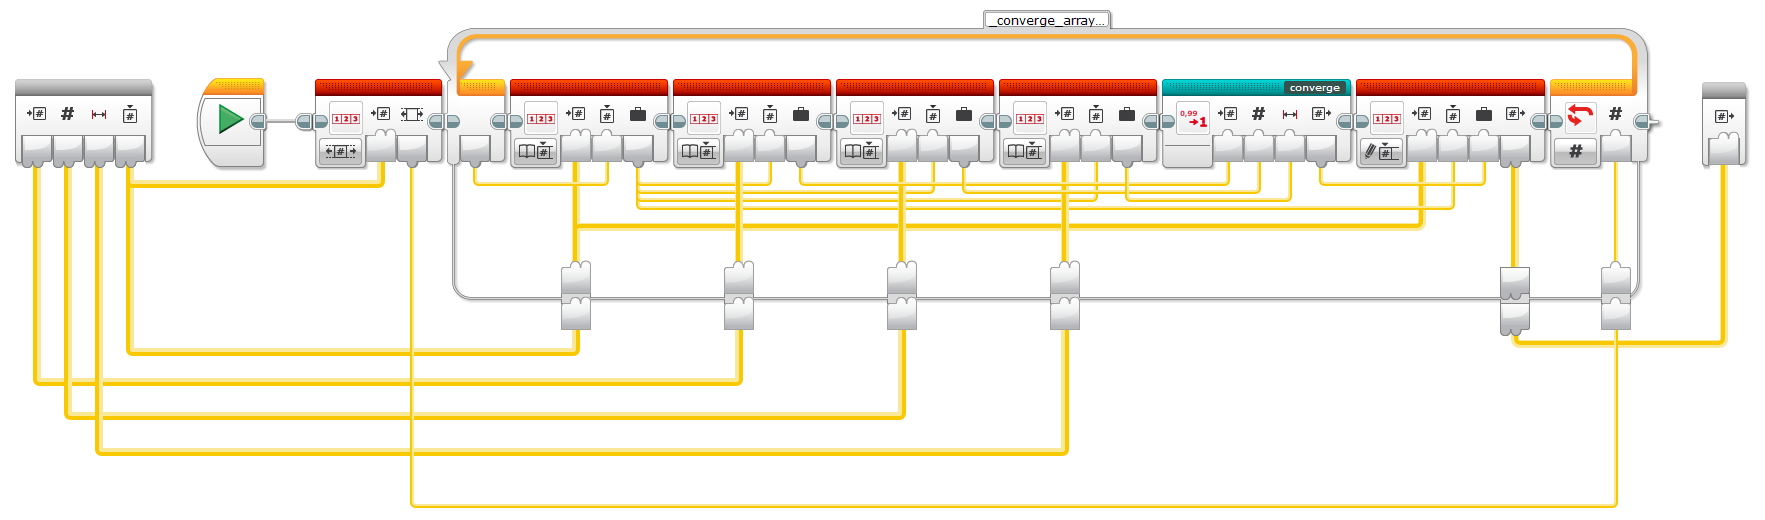
\includegraphics[width=\textwidth]{images/lego-soft_legolib_converge_array.png}
	\caption[Ukázka nepřehlednosti rozsáhlejších programů]{Ukázka nepřehlednosti rozsáhlejších programů - žluté dráhy značí předávání vstupních a~výstupních parametrů mezi jednotlivými bloky - velmi špatně se zjišťuje a~kontroluje správnost zapojení žlutých drah.}
	\label{fig:lego-soft_legolib_converge_array}
\end{figure}
 
\legoSW{} lze nainstalovat na operační systémy Windows a~Mac. K~dispozici jsou i~aplikace s~omezenými možnostmi programování pro tablety na platformě Android a~iPady.


\section{ev3dev}
\label{lego-ev3dev}

Platforma \evThreeDev{}~\cite{legoMindstormsEV3_ev3dev} je pravděpodobně nejrozšířenější a~nejrozsáhlejší alternativa k~originálnímu \lego{} prostředí.
Jedná se o~systém, drivery a~různé wrappery pro jednotlivé programovací jazyky. 
Samotný systém je založený na~linuxové distribuci Debian, který má v~sobě naportovány originální \lego{} drivery pro \EVbrick{} a~veškeré periferie.

Jelikož je \evThreeDev{} postaven na standardní linuxové distribuci, lze používat velkou škálu programovacích jazyků. 
K~dispozici jsou nízkoúrovňové jazyky C~a~C++. 
Připraveny jsou i~knihovny a~wrappery pro Python, JavaScrip, Go~\cite{legoMindstormsEV3_ev3dev-prog-lang}. 
Každý si zde může vybrat podle svých zkušeností nebo preferencí a~v~případě chuti naimplementovat i~podporu pro další jazyky. 
Aktuálně jsou stále rozpracovány implementace pro Java, Lua, Ruby,~\dots{}.

Pro práci se systémem je k~dispozici SSH~připojení, případně lze využít terminál dostupný na~úvodní obrazovce a~přes USB port si~připojit externí klávesnici. 
Tento způsob ale z~důvodu velikosti displeje na \brick{\it u} není moc komfortní. 
Systém \evThreeDev{}, na~rozdíl od~originálního \lego{} prostředí, má lepší podporu ovladačů pro WiFi a~funguje prakticky s~jakýmkoliv USB modulem. 
Systém umožňuje nastavení automatického připojování na konkrétní WiFi. Pak se již lze k~\brick{\it u} připojovat bezdrátově.
K~připojení je možné případně použít i~USB Ethernet modul.
 
Co se týče podpory \lego{} motorů a~senzorů, \evThreeDev{} zvládá obsluhovat všechny typy určené pro EV3, NXT a~některá zařízení z~WeDo~\cite{legoMindstormsEV3_ev3dev-support-motors}~\cite{legoMindstormsEV3_ev3dev-support-sensors}.
Je implementována i~široká podpora alternativních výrobců jako mindsensors.com nebo HiTechnic~\cite{baichtal2016hacking}. 
Mindsensors.com na svých webových stránkách u~některých modelů zmiňují i~podporu \evThreeDev{}~\cite{lego_mindsensor_gyro}.  

Pro zajímavost lze dodat, že tento systém podporuje i~alternativní \brick{\it y} postavené na jednodeskových počítačích Raspberry~Pi nebo BeagleBone. Příkladem komerčně prodávaných \brick{\it ů} jsou BrickPi od~Dexter Industries~\cite{lego_dexterindustries_brickpi} a~PiStorms od mindsensors.com~\cite{lego_mindsensor_pistorms}.
Obě tyto alternativy jsou postaveny na Raspberry~Pi a~umožňují připojit stejný počet standardních \lego{} motorů a~senzorů jako EV3.
Jejich hlavní výhodou je přítomnost výrazně výkonnějšího procesoru v~Raspberry~Pi. Na klasickém \brick{\it u} je totiž \evThreeDev{} dosti pomalý. 
Například samotný start systému trvá přes 60~sekund~\cite{legoMindstormsEV3_ev3dev_video-system-boot}. 
Otevření SSH spojení přes WiFi, nahrání binárního souboru do \brick{\it u} a~následné spuštění zabere až 40~sekund. 
K~tomuto zdlouhavému procesu bohužel dochází při každé změně programu. 
Díky použití Raspberry~Pi je také možné jednoduše připojit například kameru anebo přímo na GPIO piny přidat vlastní senzory (měření teploty, tlaku, vlhkosti, hodiny reálného času,~\dots).  
Mezi nevýhody můžeme počítat nemožnost účasti s~těmito alternativními \brick{\it y} soutěží, které jsou striktně omezeny na použití jen \lego{} komponent (v~České republice: \fll{}, Robosoutěž ČVUT, Robotiáda).

Avšak i~tento systém trápí podobné problémy jako originální \lego{} prostředí. 
Hlavním nedostatkem je, že~Linux nemá standardně real-time kernel. 
% Linux -> scheduler -> spravedlivý -> negarantuje čas, ale optimální využití procesoru
% real-time -> není spravedlivý ale umožňuje přesné časování jednotlivých tasku a přesné cyklické spouštění tasku -> nedochází k optimálnímu využití procesoru
Není tak garantováno přesné přidělování výpočetního času pro uživatelské programy, což je velký problém pro běh různých regulačních smyček, které potřebují konstantní dobu mezi jednotlivými průběhy (například stabilizace samobalancujícího robota). 
V~\evThreeDev{} dle měření dochází až k~20~ms prodlevám, kdy si kernel zabere výpočetní čas a~uživatelská aplikace se nedostane k~vykonávání programu~\cite{legoMindstormsEV3_ev3dev-issue_constant-loop-time}. 
Jedno z~řešení je výrazně zpomalit regulační smyčku, ale ani to negarantuje, že se program dostane k~vykonávání v~požadovaný čas.
V~rámci \evThreeDev{} proběhl pokus o~zakomponování real-time kernelu do separátní vývojové větve.~\cite{legoMindstormsEV3_ev3dev-rt-kernel-start}. 
Jelikož se ale tato větev potýkala s~problémy ovladačů motorů, byl její vývoj ukončen~\cite{legoMindstormsEV3_ev3dev-rt-kernel-end}.  
% TODO: scheduler v EV3 -  https://github.com/ev3dev/ev3dev/issues/324
%Určité výtky lze mít i~vůči implementaci driverů pro motory, kde se většina nastavování provádí přes textové řetězce (viz~obrázek~\ref{src:ev3dev-lang-cpp_drive-test}). 
%Určitě se nejedná o nejrychlejší řešení.


\begin{figure}[H] 
	\begin{minted}[xleftmargin=1.5em,linenos=true]{cpp}
if(motor.speed_regulation_enabled() == "off")
    motor.set_speed_regulation_enabled("on");
motor.set_speed_sp(speed);
motor.run_forever();
	\end{minted}
	\caption{Ukázka nastavení rychlosti motoru v~implementaci C++ na \evThreeDev}
	\label{src:ev3dev-lang-cpp_drive-test}
\end{figure}

Co považuji za~další problém, je roztříštěnost této platformy a~náročnost pro méně zkušené uživatele. 
Jednotlivé implementace programovacích jazyků mají různorodou kvalitu dokumentace a~většinou relativně složité rozhraní. 
Na obrázku~\ref{src:ev3dev-lang-cpp_drive-test} je ukázka kódu pro nastavení rychlosti jednoho motoru v~C++~na~\evThreeDev{}. 
Pro další inspiraci je možné se podívat na~demo příklady k~tomuto API~\cite{legoMindstormsEV3_ev3dev-lang-cpp_drive-test}.
Bohužel pro člověka, který doposud programoval pouze přes \lego{} prostředí, je podle mě toto rozhraní velmi složité.

%Jelikož mám na~\evThreeDev{} největší zkušenosti s C++~API, tak bych chtěl poukázat na nedostatky v tomto API. 
%Zároveň by u~C++ nemělo docházet k~degradaci výkonu, což může nastávat u interpretovaných jazyků jako Python nebo JavaScript. 
Příklad v~C++~API jsem vybral z~důvodu svých předešlých zkušenosti s~tímto rozhraním a~předpokladu, že by u~C++ nemělo docházet k~degradaci výkonu, což by mohlo nastávat u~interpretovaných programovacích jazyků jako Python nebo JavaScript.

Ze~svých dlouhodobých zkušeností se~začátečníky mám dobrou představu, jakých chyb se nejčastěji dopouští a~co jim dělá největší problém.
Proto jsem se v~rámci testování \evThreeDev{} podílel i~na tvorbě knihovny~\cite{legoMindstormsEV3_ev3dev_RB-ev3dev-cpp-lib}, která byla vyvíjena se záměrem co nejvíce usnadnit uživateli programování robotů v~\evThreeDev{}. 
Přestože tato knihovna mnohé neduhy programování na tomto systému odstraňuje, stále tu přetrvává celá řada problémů souvisejících s~použitím linuxového systému (viz popis v~úvodu této kapitoly).


Při zkoumání API pro Python~\cite{legoMindstormsEV3_ev3dev-lang-python} jsem došel k~podobnému závěru. 
Je pravda, že k~němu lze najít rozsáhlejší dokumentaci~\cite{legoMindstormsEV3_ev3dev-lang-python-docs}. 
I~tak není dle mého názoru pro programátora~-- začátečníka, který přechází z~\lego{}  softwaru, toto API dostatečně jednoduché a~intuitivní.


\section{ROS}

S~\legoEV{} je možné používat i~ROS (Robot Operating System)~\cite{legoProgramingPlatform_ROS}. 

ROS je platforma určená přímo pro robotiku a~roboty. 
Jde o~systém, který v~sobě integruje nástroje pro komunikaci, loggování, zpracování obrazu, navigaci, simulace nebo ovládání zařízení. 
Uživateli značně usnadňuje obsluhu vlastního robota, protože má předpřipraveno již mnoho nástrojů.

Na samotném EV3 kvůli nedostatečnému výkonu \brick{\it u}  kompletní ROS neběží.
Pro EV3 ale existuje utilita do systému \evThreeDev{}, přes kterou lze pomocí příkazů komunikovat s~ROSem běžícím na standardním PC. 
Tím lze získávat data ze senzorů a~posílat zpět instrukce pro motory. 
Komunikace mezi PC a~\EVbrick{\it em} může probíhat po WiFi nebo Ethernetu.
Veškerá logika jako plánování trasy, herní strategie, případně zpracování dat je prováděna v~rámci klasického~PC.
Hlavními důvody pro použití ROSu na EV3 je široká paleta balíčků, které řeší například práci s~různými senzory jako kamera, Kinect, lidar, ale i~ovládacích zařízení typu joystick či gamepad. 
Zároveň je v~ROSu integrována transformace souřadnic, plánování trasy, herní strategie nebo i~simulátor s~fyzikálním enginem.


Při využívání ROSu společně se stavebnicí \lego{} je ovšem problematická nutnost mít k~\brick{\it u} připojené klasické PC. 
Jak bylo již uvedeno v~kapitole~\ref{lego-ev3dev}, mnoho soutěží pro \legoM{} vyžaduje striktní použití jen \lego{} komponent, a~to běžné PC není. 
Zároveň i~soutěže, které nemají tuto podmínku, například Robotický den v~Praze nebo Istrobot v~Bratislavě, zakazují spojení s~jakýmkoliv externím zařízením.
Tím pádem je nutné, aby na sobě \lego{} robot vozil klasické PC, což může značně zvýšit hmotnost a~náročnost konstrukce. 
V~dnešní době by to ovšem již neměl být takový problém (např. lze použít Raspberry~Pi anebo zařízení založené na~Intel Atom).

\section{Balíček od MathWorks}
\label{lego-alternative-soft_mathworks}

MathWorks pro \legoM{} připravil doplňky do svých programů Mat\-lab a~Simulink. 
Cílem těchto doplňků je umožnit uživateli ovládat a~programovat \legoM{} ve standardním MathWorks prostředí. 
V~rámci balíčků je podporováno \legoNXT~\cite{legoProgramingPlatform_MathWork-NXT} i~EV3~\cite{legoProgramingPlatform_MathWork-EV3}.
Uživatel může ovládat \brick{} pomocí příkazů z~Mat\-la\-bu anebo lze program vytvořit formou diagramů v~Simulinku (podobně jako v~oficiálním \lego{} prostředí). 
Příklad programu pro sledování čáry lze vidět na obrázku~\ref{fig:mathworks-simulink_line-tracking-model}.
Programy v~Simulinku vypadají srozumitelně a~přehledně, ale vzhledem k~povaze samotného prostředí (laboratorní až~vědecký simulační nástroj) není jeho ovládání a~tvorba aplikací jednoduchá a~pro nováčka občas až odrazující. 

\begin{figure}[h]
	\centering
	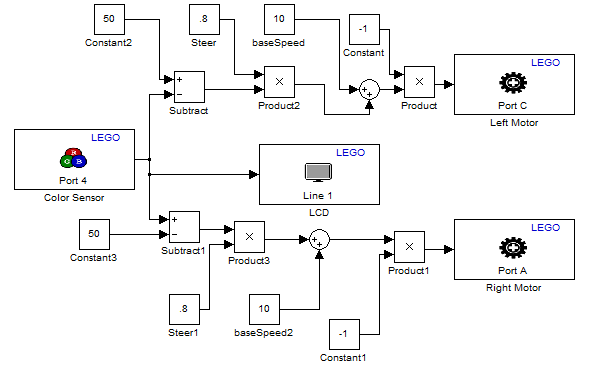
\includegraphics[width=330px]{images/mathworks-simulink_line-tracking-model.png}
	\caption[Program na sledování čáry v~prostředí Simulink]{Program na sledování čáry v~prostředí Simulink\protect\footnotemark}
	\label{fig:mathworks-simulink_line-tracking-model}
\end{figure}

\footnotetext{Zdroj: \url{http://blogs.mathworks.com/simulink/2012/03/05/running-simulink-models-on-lego-mindstorms-nxt/}} 

Doplňky ke~svému fungování využívají standardní \lego{} systém. 
Proto se při ovládání \brick{\it u} z~Matlabu posílají příkazy, které \lego{} připravilo pro vzdálené řízení. 
EV3 tyto příkazy běžně využívá v~režimu Daisy-Chain, kdy lze USB kabely spojit do série až~čtyř \brick{\it ů} a~řídit je jedním programem.     

Při návrhu programu v~Simulinku se vytváří ekvivalentní byte-code uživatelská aplikace, která se do \brick{\it u} nahrává stejně jako program ze standardního \lego{} prostředí. 
Z~toho vyplývá, že vlastnosti a~chování programů vytvořených v~Matlabu a~Simulinku budou ekvivalentní se standardními programy z~\lego{} prostředí.

Problém balíčku od MathWorksu je i~cena licencí za~jejich software. 
Standardně se pohybuje v~řádech deseti tisíců korun za~jednu licenci~\cite{legoProgramingPlatform_MathWork_Humusoft-price}.
To je pro běžného uživatele nepřijatelná částka. 
MathWorks nabízí i~speciální licence pro školy za~výrazně lepší ceny. 
K~této licenci se ovšem běžný uživatel nedostane, a~proto jsem toto prostředí dále nezkoumal.
Doplňky jsou dostupné pro Windows, Mac i~Linux. 
 

\section{Balíček od \NI}

I~firma \NI{} nabízí modul pro \legoM{} do svého programu \labview{}~\cite{legoProgramingPlatform_NI_LabVIEW}. 
Funkcionalitou i~vlastnostmi se velmi podobá doplňkům od MathWorks~\cite{garber2015learning}.
Taktéž využívá standardní \lego{} systém a~platí pro něj tedy vše, co je popsáno v~kapitole~\ref{lego-alternative-soft_mathworks} věnující se doplňkům pro Matlab a~Simulink. 
Cena licencí je také obdobná. Modul je dostupný pro Windows a~Mac. 


\section{ROBOTC}

ROBOTC je programovací jazyk pro roboty založený na jazyku~C. 
Zároveň se jedná o~platformu podporující různé robotické systémy jako \legoM{} (RXC, NXT, EV3), Arduino, VEX Robotics, PIC a~další~\cite{legoProgramingPlatform_ROBOTC}.
Jde o~komerční produkt, který je přímo zaměřen na hobby robotiku.
Na trhu je již dlouhou dobu a~v~minulosti byl hojně využíván pro programování \legoNXT{}.
Nabízí zajímavou kombinaci grafického a~textového programování. 
Grafické programy (ROBOTC Graphical) mají podobný vizuální styl jako Scratch~\cite{scratch_oficial-about} (jeden z~nejrozšířenějších grafických programovacích jazyků určený pro výuku programování -- oficiální webové stránky aktuálně navštíví každý měsíc kolem 17 miliónů uživatelů~\cite{scratch_oficial-statistic}). 
U~textových programů lze volit míru abstrakce, nad kterou se pracuje (ROBOTC~NL /~ROBOTC). 
Mezi grafickým a~textovým režimem se bohužel nelze přepínat.

Součástí prostředí je i~simulátor pro testování programů bez potřeby hardwaru. 
Uživatel tak může jednoduše ladit program, aniž by měl u~sebe fyzicky robota.
Této možnosti mohou využít zvláště týmy připravující se na určitou soutěž. 
Část týmu může stavět nebo upravovat hardware, zatímco ostatní mohou ladit program ve~virtuálním prostředí. 

\begin{figure}[h]
	\centering
	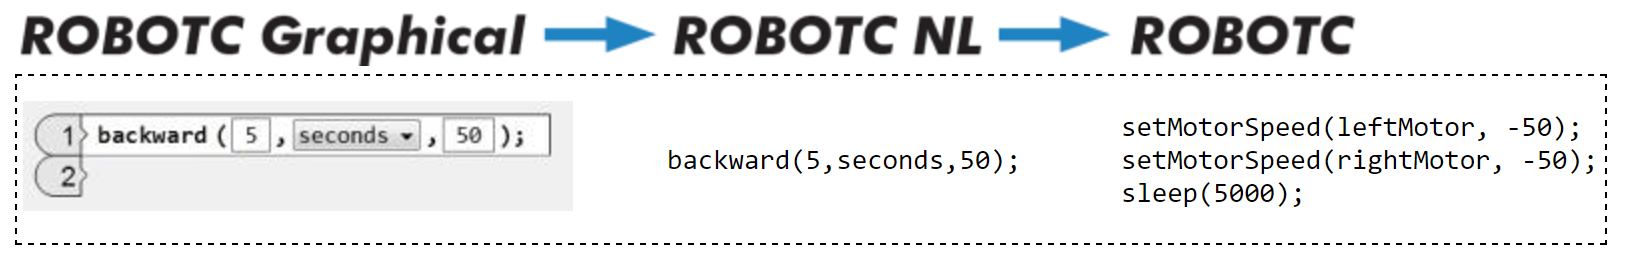
\includegraphics[width=330px]{images/robotc_language-variants.png}
	\caption[ROBOTC nabízí tyto varianty programování]{ROBOTC nabízí tyto varianty programování\protect\footnotemark} % CHECK: programování / programovacích jazyků
	\label{robotc_language-variants}
\end{figure}

\footnotetext{Zdroj: Oficiální nápověda v~programu ROBOTC -- záložka ROBOTC Language Progression} 

ROBOTC běží na standardním \lego{} systému podobně jako doplňky od~MathWorks nebo \NI{}.
Programy z~ROBOTC se na PC překládají do~byte-code aplikací a~následně se spouští na \brick{\it u} ve~virtuálním stroji. 
Tudíž zde může docházet k~podobným problémům, jako je popsáno v~kapitole~\ref{lego-soft-orig-problems}.

V~rámci vývojového programu pro toto prostředí je k~dispozici celá řada podpůrných nástrojů typu debugger, dataloger, vykreslování grafů nebo i~ovládání robota přes joystick.
Samotné prostředí je relativně propracované a~obsahuje mnoho funkcí. 
Aktuální verze by si zasloužila grafické přepracování tak, aby byla intuitivnější. 
Je trochu škoda, že není k~dispozici implementace jazyka ROBOTC v~C++ stylu, ale vzhledem k~dobré koncepci současného jazyka to asi není nutné. 

Jak bylo uvedeno v~úvodu, ROBOTC je komerční program, a~s~tím souvisí licenční politika. 
Ceny licencí s~platností na jeden rok jsou přibližně poloviční v~porovnání s~časově neomezenými verzemi.
Neomezená verze dle jednotlivých balíčků stojí: \$79, \$299, \$599~\cite{legoProgramingPlatform_ROBOTC-price}.  
V~porovnání s~produkty od MathWorks nebo \NI{} nejsou tyto sumy tak závratné a~když zvážíme cenu samotné stavebnice \legoEV{} (aktuálně 11 700 Kč~\cite{lego_eduxeEshop_CoreSet}, v~přepočtu přibližně~\$470), zdá se mi tato suma přijatelná.

I~tak může být cena za tento produkt pro mnohé uživatele, školy a~vzdělávací instituce rozhodující.
Zároveň kvůli uzavřenosti tohoto softwaru není možné jednoduše rozšiřovat funkcionalitu a~přidávat další vylepšení do programu. 
Vzhledem k~výše uvedeným důvodům jsem se rozhodl, že pro svou práci nebudu toto prostředí dále zvažovat.	


\section{EV3RT}
\label{lego-EV3RT}

Při hledání příčin problémů s~časováním na EV3~\cite{legoMindstormsEV3_ev3dev-issue_constant-loop-time} jsem narazil na zajímavý japonský projekt \evRT{}~\cite{legoProgramingPlatform_EV3RT-git-web}.
Jedná se o~port real-timového systému TOPPERS/HRP2 na \legoEV{}.
Projekt \evRT{} vznikl v~rámci výzkumu na Nagoya University v~Japonsku s~cílem odstranění problémů originálního \lego{} systému a~prostředí. 
Veškeré zdrojové kódy jsou volně k~dispozici na GitHubu~\cite{legoProgramingPlatform_EV3RT-github}. 

Historie projektu TOPPERS\footnote{TOPPERS = Toyohashi OPen Platform for Embedded Real-time Systems} sahá do roku 2003, kdy vznikl jako společný projekt průmyslu, univerzit a~vlády~\cite{legoProgramingPlatform_TOPPERS}. 
Cílem projektu bylo vytvoření kvalitního otevřeného real-time systému, využitelného v~průmyslu pro embedded zařízení. 
Zároveň měly být vytvořeny výukové kurzy a~materiály pro studenty.
V~Japonsku je tento systém využíván jak v~průmyslu, tak i~při výuce a~prakticky tvoří průmyslový standard pro embedded zařízení. 

TOPPERS je vyvíjen s~celou řadou real-time kernelů. Pro EV3 byl portován kernel s~označením HRP2\footnote{HRP2 = High Reliable system Profile version 2}.
Jedná se o~statický RTOS\footnote{RTOS = Real-Time Operating System} kernel s~podporou ochrany paměti, který splňuje vysokou spolehlivost a~bezpečnost aplikací~\cite{legoProgramingPlatform_EV3RT-paper}.
V~systému je možné vytvářet tasky (obdoba vláken v~Linuxu) s~různou prioritou. 
Jsou zde dostupné standardní prostředky pro komunikaci mezi tasky: semafory, mutexy, fronty.

\begin{figure}[h]
	\centering
	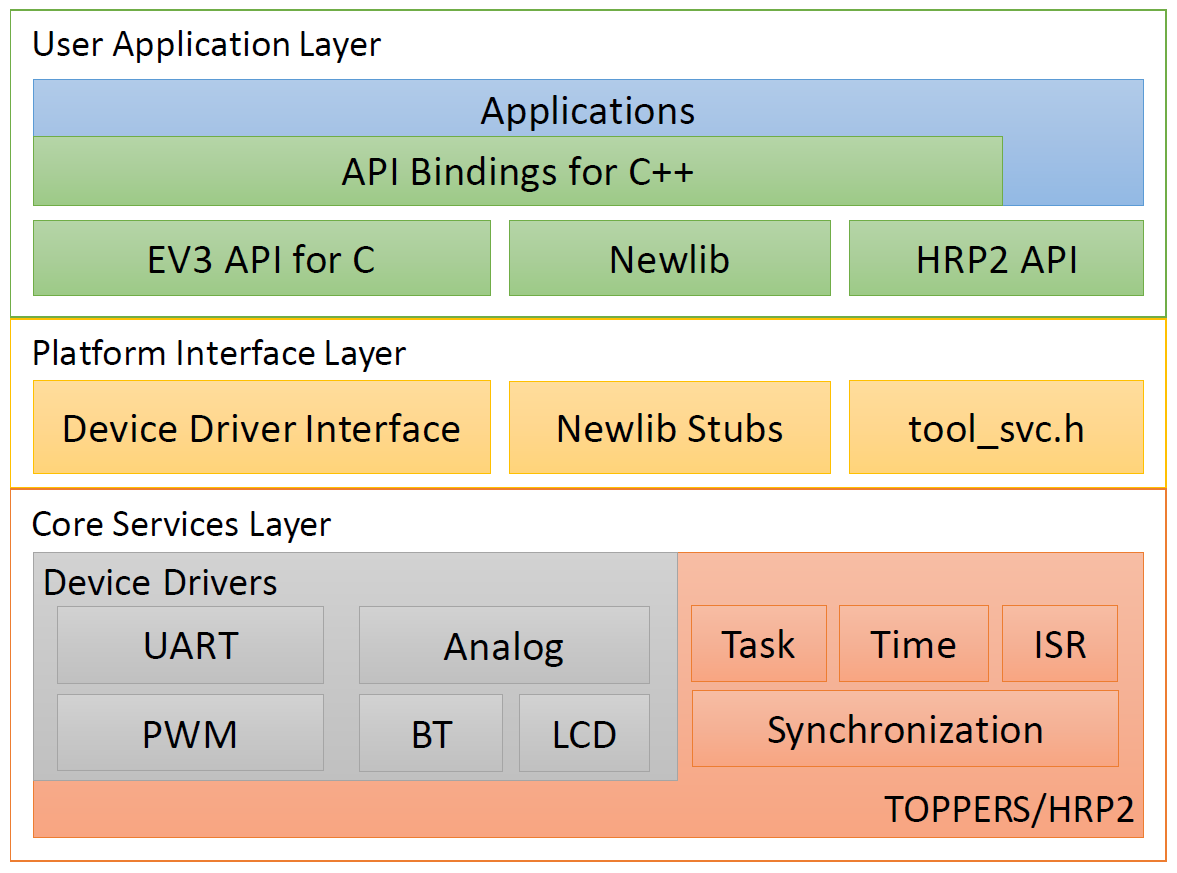
\includegraphics[width=330px]{images/ev3rt-architecture.png}
	\caption[Architektura systému EV3RT]{Architektura systému EV3RT\protect\footnotemark}
	\label{ev3rt-architecture}
\end{figure}

\footnotetext{Zdroj: článku A~Platform for LEGO Mindstorms EV3 Based on an RTOS with MMU Support~\cite{legoProgramingPlatform_EV3RT-paper}} 

V~rámci EV3RT jsou aktuálně podporovány všechny druhy senzorů a~motorů ze~stavebnice \legoEV{} a~fungují veškeré periferie na~\EVbrick{\it u} (displej, LED, tlačítka, Bluetooth a~reproduktor). 
Zatím není odzkoušená podpora pro NXT komponenty ani alternativní senzory a~motory. 

EV3RT poskytuje C~API pro přístup ke~všem funkcím na EV3. 
Jednoduše lze vyčíst hodnoty ze senzoru nebo roztočit motor.
Toto API není ale tak intuitivní, jak by mohlo být při použití C++.
K~dispozici je i~implementace dynamické alokace paměti a~lze tedy používat funkce \verb|malloc()| i~\verb|free()|.
Platforma nemá problém s~překladem standardní C++~knihovny (STL).
Uživatel tak může v~projektech využívat například \texttt{std::string}, \texttt{std::vector}, \texttt{std::queue}, \texttt{\dots}

Výkonnostně by na tom měl být systém EV3RT nejlépe ze všech platforem pro EV3, které byly zmíněny v~této kapitole. 
Hlavní příčinou je samotný RTOS, který má velmi nízkou režii na svůj chod a~umožňuje rychlý přístup k~hardwaru. % TODO: + rychlejší zpracování operaci a přepínání tasku
Oproti standardnímu \lego{} systému zde také neběží žádný virtuální stroj, který může výrazně degradovat výkon při některých operacích. 
Dle testů provedených tvůrci EV3RT je například provedení nastavení rychlosti ({\it motor\_set\_speed}) v~průměru až 100krát
 rychlejší než v~originálním systému~\cite{legoProgramingPlatform_EV3RT-paper}. \\
 
Shrnutí hlavních vlastností \evRT:

\begin{itemize}
	\item malá velikost systému (do 5 MB) i~uživatelských aplikací (do 1 MB)
	\item velmi rychlý start (do 5 sekund) a~prakticky okamžité vypnutí
	\item jednodušší úprava a~doprogramování vlastních funkcí do jádra systému
	\item snadné portování linuxových driverů
	\item podpora dynamické alokace paměti
	\item preemptivní multitasking s~velmi rychlým přepínáním kontextu (do 8 $\mu$s)
	\item multiplatformní vývoj aplikací pro EV3
\end{itemize}
 
Nevýhodou TOPPERS a~tedy i~EV3RT je, že se jedná primárně o~japonský projekt. 
Většina dokumentace k~TOPPERS je tak v~japonštině, což se týká i~velké části zdrojového kódu v~EV3RT. 
Části kódu, které byly převzaty z~oficiálního \lego{} systému nebo byly vytvářeny primárně pro EV3RT, jsou zdokumentovány v~angličtině. 

Například ale C~API obsahuje pouze japonskou dokumentaci.
Jedinou anglickou dokumentací k~funkcím dostupných v~TOPPERS/HRP2 je tak všeobecná RTOS specifikace $\mu$ITRON z~roku 2002~\cite{legoProgramingPlatform_TOPPERS-IRON}, kterou HRP2, a~tím pádem i~EV3RT, splňují. % splňují/implementují
Naštěstí překlad z~japonštiny do angličtiny zvládá Google Translate docela dobře, a~tak je možné tyto komplikace překonat.


Ačkoliv má EV3RT určité nevýhody popsané v~předchozím odstavci, rozhodl jsem se jej využít pro tvorbu programovacího prostředí pro \legoEV{}.
Tento systém jako jediný nabízí opravdovou real-timovost.
Netrpí degradací výkonu.
Zvládne velmi rychle nastartovat a~okamžitě se vypne. 
Nabízí relativně snadnou možnost zásahů do implementace (úpravu driverů pro EV3 -- úprava konstant PID~regulátoru, modifikace a~přidávání funkcí do uživatelského rozhraní, \dots). 

Pro EV3RT lze vyvíjet na libovolné POSIX-kompatibilní platformě obsahující GCC překladač pro procesory ARM. Vývoj je tedy možný jak na Linuxu a~Macu, tak i~na Windows s~použitím Cygwinu~\cite{legoProgramingPlatform_EV3RT-git-web_get-started}.


\section{Srovnání dostupných platforem}
\label{lego-soft-summary}

V~této kapitole shrnuji porovnání jednotlivých platforem mezi sebou. 
Vybral jsem několik bodů, které považuji za~důležité u~platformy určené pro programování stavebnice \lego{}. 
Zároveň by tyto body měly zohledňovat možnosti budoucího rozvoje daného prostředí a~snadné využití platformy ve~výuce. \\


Platformy budu posuzovat v~těchto bodech:

\begin{enumerate}
	\item dostupné zdarma
	\item open-source
	\item intuitivní programovací rozhraní pro neprogramátory
	\item nenáročnost na počáteční zprovoznění
	\item real-timovost
	\item nenáročné na hardware počítače
	\item možnost zásahů do vývojového prostředí
	\item podporované operační systémy
\end{enumerate}


\begin{center}
	\begin{tabular}{ | l | c | c | c | c | c | c | c | c |}
		\hline
		Prostředí:                  & 1      & 2      & 3      & 4      & 5      & 6      & 7     	& 8							\\ \hline
		Originální \lego{}          & \Has   & \NoHas & \Has   & \Has   & \NoHas & \NoHas & \NoHas 	& Windows, Mac	\\ \hline 
		\evThreeDev{}               & \Has   & \Has   & \NoHas & \NoHas & \NoHas & \Has   & \Has 	& Windows, Linux, Mac		\\ \hline 
		ROS 						& \Has   & \Has   & \NoHas & \NoHas & \NoHas & \NoHas & \Has 	& Linux						\\ \hline 
		MathWorks doplňky           & \NoHas & \NoHas & \NoHas & \Has   & \NoHas & \NoHas & \NoHas  & Windows, Linux, Mac		\\ \hline 
		\NI{} modul                 & \NoHas & \NoHas & \NoHas & \Has   & \NoHas & \NoHas & \NoHas  & Windows, Mac				\\ \hline
		ROBOTC		                & \NoHas & \NoHas & \Has   & \Has   & \NoHas & \Has   & \NoHas  & Windows					\\ \hline
		EV3RT			            & \Has   & \Has   & \NoHas & \NoHas & \Has   & \Has   & \Has   	& Windows, Linux, Mac		\\ \hline
	\end{tabular}
\end{center}

Z~výše uvedené tabulky i~hlubšího zkoumání jednotlivých prostředí v~rámci této kapitoly mi~jako nejvhodnější volba pro programování stavebnice \legoEV{} připadá prostředí EV3RT.
Má některé nedostatky, které u~jiných prostředí nejsou (složitější API, náročné na počáteční zprovoznění), ale právě tato problematická místa by mělo být možné díky otevřenému zdrojovému kódu odstranit.
Proto se již budu v~následujících kapitolách věnovat převážně tomuto systému.
      
  \chapter{Testování}
\label{testing}

Cílem testování v~této kapitole je zjistit výkonnost jednotlivých platforem a~porovnat je vůči sobě. 
Testy jsou zaměřeny primárně na měření časů průběhu hlavní smyčky při určitých činnostech tak, aby bylo možné srovnat výkonnost a~stabilitu jednotlivých platforem. 
Stabilitou je v~tomto případě myšlen rozdíl mezi průměrným a~maximálním naměřeným časem průchodu smyčky v~rámci opakovaných měření a~jednotlivých průchodů.

Při předchozí práci s~\EVthree{ } se systémem \evThreeDev (viz kapitola~\ref{lego-ev3dev}), že minimální perioda hlavní smyčky s~pár příkazy na vyčtení dat ze senzoru a~následného nastavení motorů dle těchto hodnot (klasický program na jízdu po čáře) není kratší než 10~ms. 
Vzhledem k~výkonu procesoru (32bitový ARM na 300~MHz) v~\EVthree{ }je tento čas velmi zarážející. 

O~to větší překvapení nastalo, když jsem srovnával průměrnou periodu s~maximální. Ukázalo se, že ačkoliv je průměrná perioda přibližně 20~ms, maximální perioda může dosahovat až~100~ms. 
Takto velký rozptyl je pro potřeby regulace velmi problematický. 
Ve většině případů je potřeba mít konstantní čas průchodu hlavní smyčkou, aby rozdíl v~časech periody neovlivňoval měření a~následné řízení. 

Pokud bude nutné zajistit stabilní periodu, je třeba softwarově zpomalit průběh hlavní smyčky na maximální naměřený čas. 
Jedině tak lze zajistit konstantní periodu. 
Když by se použil tento postup, dostali bychom se na frekvenci 10~Hz, což je z~pohledu regulace již velmi nepříznivá hodnota.

Tyto testy byly provedeny na velmi jednoduchém programu. 
V~případě rozsáhlejších projektů, kde by se pracovalo s~více vlákny a~periferiemi, mohou být výsledky ještě horší.

Proto jsem chtěl provést testování s~ekvivalentními programy na jednotlivých platformách a~zjistit, jestli tyto neduhy některá z~nich neodstraňuje a~za jakých situací k~podobným problémům dochází.

\section{Forma testování}

Na počátku jsem zvažoval dvě formy testování. První počítala s~rozsáhlejší metodikou, v~rámci které bych testoval různé funkce \EVthree{}~\brick{{\it u}} a~zjišťoval, kde mohou být nejproblémovější místa z~pohledu výkonu. \\

V~rámci testů jsem se chtěl zaměřit na několik oblastí: % a jejich kombinace.

\begin{itemize}
	\item matematické operace
	\item čtení senzorů
	\item řízení motorů
\end{itemize}  

Tuto variantu jsem na počátku odložil, abych zkusil najít metodu jednoduší na implementaci a~replikaci na jiné platformy. Následně v~ní ale pokračuji v~další části kapitoly.

Druhá varianta měla zajistit co možná nejstejnoměrnější podmínky měření času tak, aby jej neovlivňovalo fungování jednotlivých platforem. 
Proto mělo být k~měření využito Arduino Uno a~velmi jednoduchý program  (příklad programu ve standardním prostředí pro \EVthree{ }na obrázku \ref{fig:LoopTimeLEDblinking-measuring}).
Program by jen blikal s~dvěma LED\footnote{LED = Light-Emitting Diode –- dioda emitující světlo} (zelenou a~červenou) umístěnými na přední straně pod ovládacími tlačítky na \EVbrick{{\it u}} a~čas svitu jednotlivých LED by měřilo Arduino.

%U jednotlivých platforem by se měřili časy průchodů hlavní smyčkou a z těchto naměřených dat by se vytvářeli histogramy pro následné vyhodnocení.

% Následně jsem se ale rozhodl pro jinou strategii testování. 
% Rozhodl jsem se ale pro jinou strategii testování. 

% Po čase jsem tuto strategii zavrhl. 

Jednalo by se totiž o~jeden z~nejlepších způsobů, jak demonstrovat problémy s~dobou trvání jednotlivých cyklů a~práci s~periferiemi. 
V~optimálním případě by totiž měla kombinací těchto dvou barevných LED vzniknout oranžová. 

Pokud by se tak nestalo, pozorovatel by měl hned optickou zpětnou vazbu a~zároveň lze jednoduše měřit časové prodlevy mezi spínáním a~vypínáním jednotlivých LED pomocí měřicí sestavy s~Arduinem.

\section{Měření pomocí LED}


\begin{figure}[h]
	\centering
	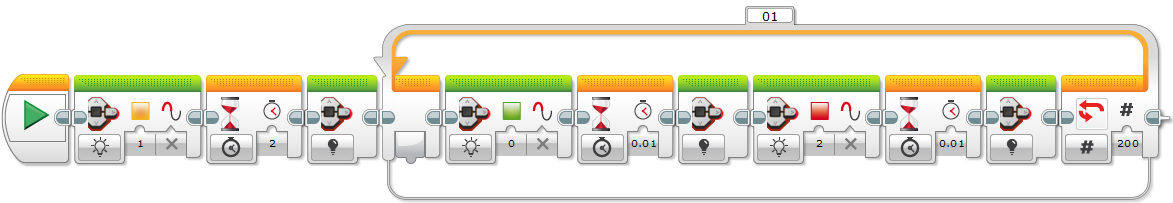
\includegraphics[width=\textwidth]{images/measuring-ev3-software_LoopTimeLEDblinking.png}
	\caption[Ukázka jednoduchého programu na blikání zelenou a~červenou LED]{Ukázka jednoduchého programu na blikání zelenou a~červenou LED}
	\label{fig:LoopTimeLEDblinking-measuring}
\end{figure}

Ukázkový program je připraven tak, že každá LED se vždy rozsvítí na 10~ms ($T~=~0.01~s~= 10~ms$), následně zhasne a~rozsvítí se druhá LED. 

Celkový čas jednoho průchodu cyklem trvá 20~ms ($T~=~T_{LED1}~+ T_{LED2}$) a~frekvence blikání by měla být 50~Hz ($f~=~\frac{1}{T}~= \frac{1}{0.02~s} =~50~Hz$). 
Což je frekvence, kterou již lidské oko nezaznamená (filmy mají standardní frekvenci obnovování snímku 24 až 30~Hz). % TODO: a běžné televizní vysílání má 50~Hz).
Celkový počet opakování hlavní smyčky je zvolen na 200. 
Blikání má tedy probíhat 4~sekundy ($t~=~T~\cdot~counter =~0.02~ms~\cdot~200~= 4~s$).

Pro měřicí sestavu byl vybrán fototranzistor BPX~81\footnote{\url{http://cz.rs-online.com/web/p/fototranzistory/6655255/}} (má velmi široké rozpětí vstupních vlnových délek -- zvládne viditelné i~infra světlo) s~Arduinem Uno (viz obrázek~\ref{fig:arduino-measuring-system}). \\

Tato kombinace mi přijde nejvhodnější z~několika důvodů: 

\begin{itemize}
	\item velmi rozšířený hardware (Arduino Uno)
	\item rychlé sestavení
	\item možnost snadného naprogramování
	\item jednoduchá duplikovatelnost (zopakování experimentu)
\end{itemize}  

Nejdůležitějším bodem pro tuto variantu byla jednoduchá duplikovatelnost, která umožňuje komukoliv provést stejná měření, ať už pro kontrolu v~této práci prezentovaných výsledků, nebo pro otestování jiné platformy a~porovnání s~naměřenými daty z~této práce.

\begin{figure}[h]
	\centering
	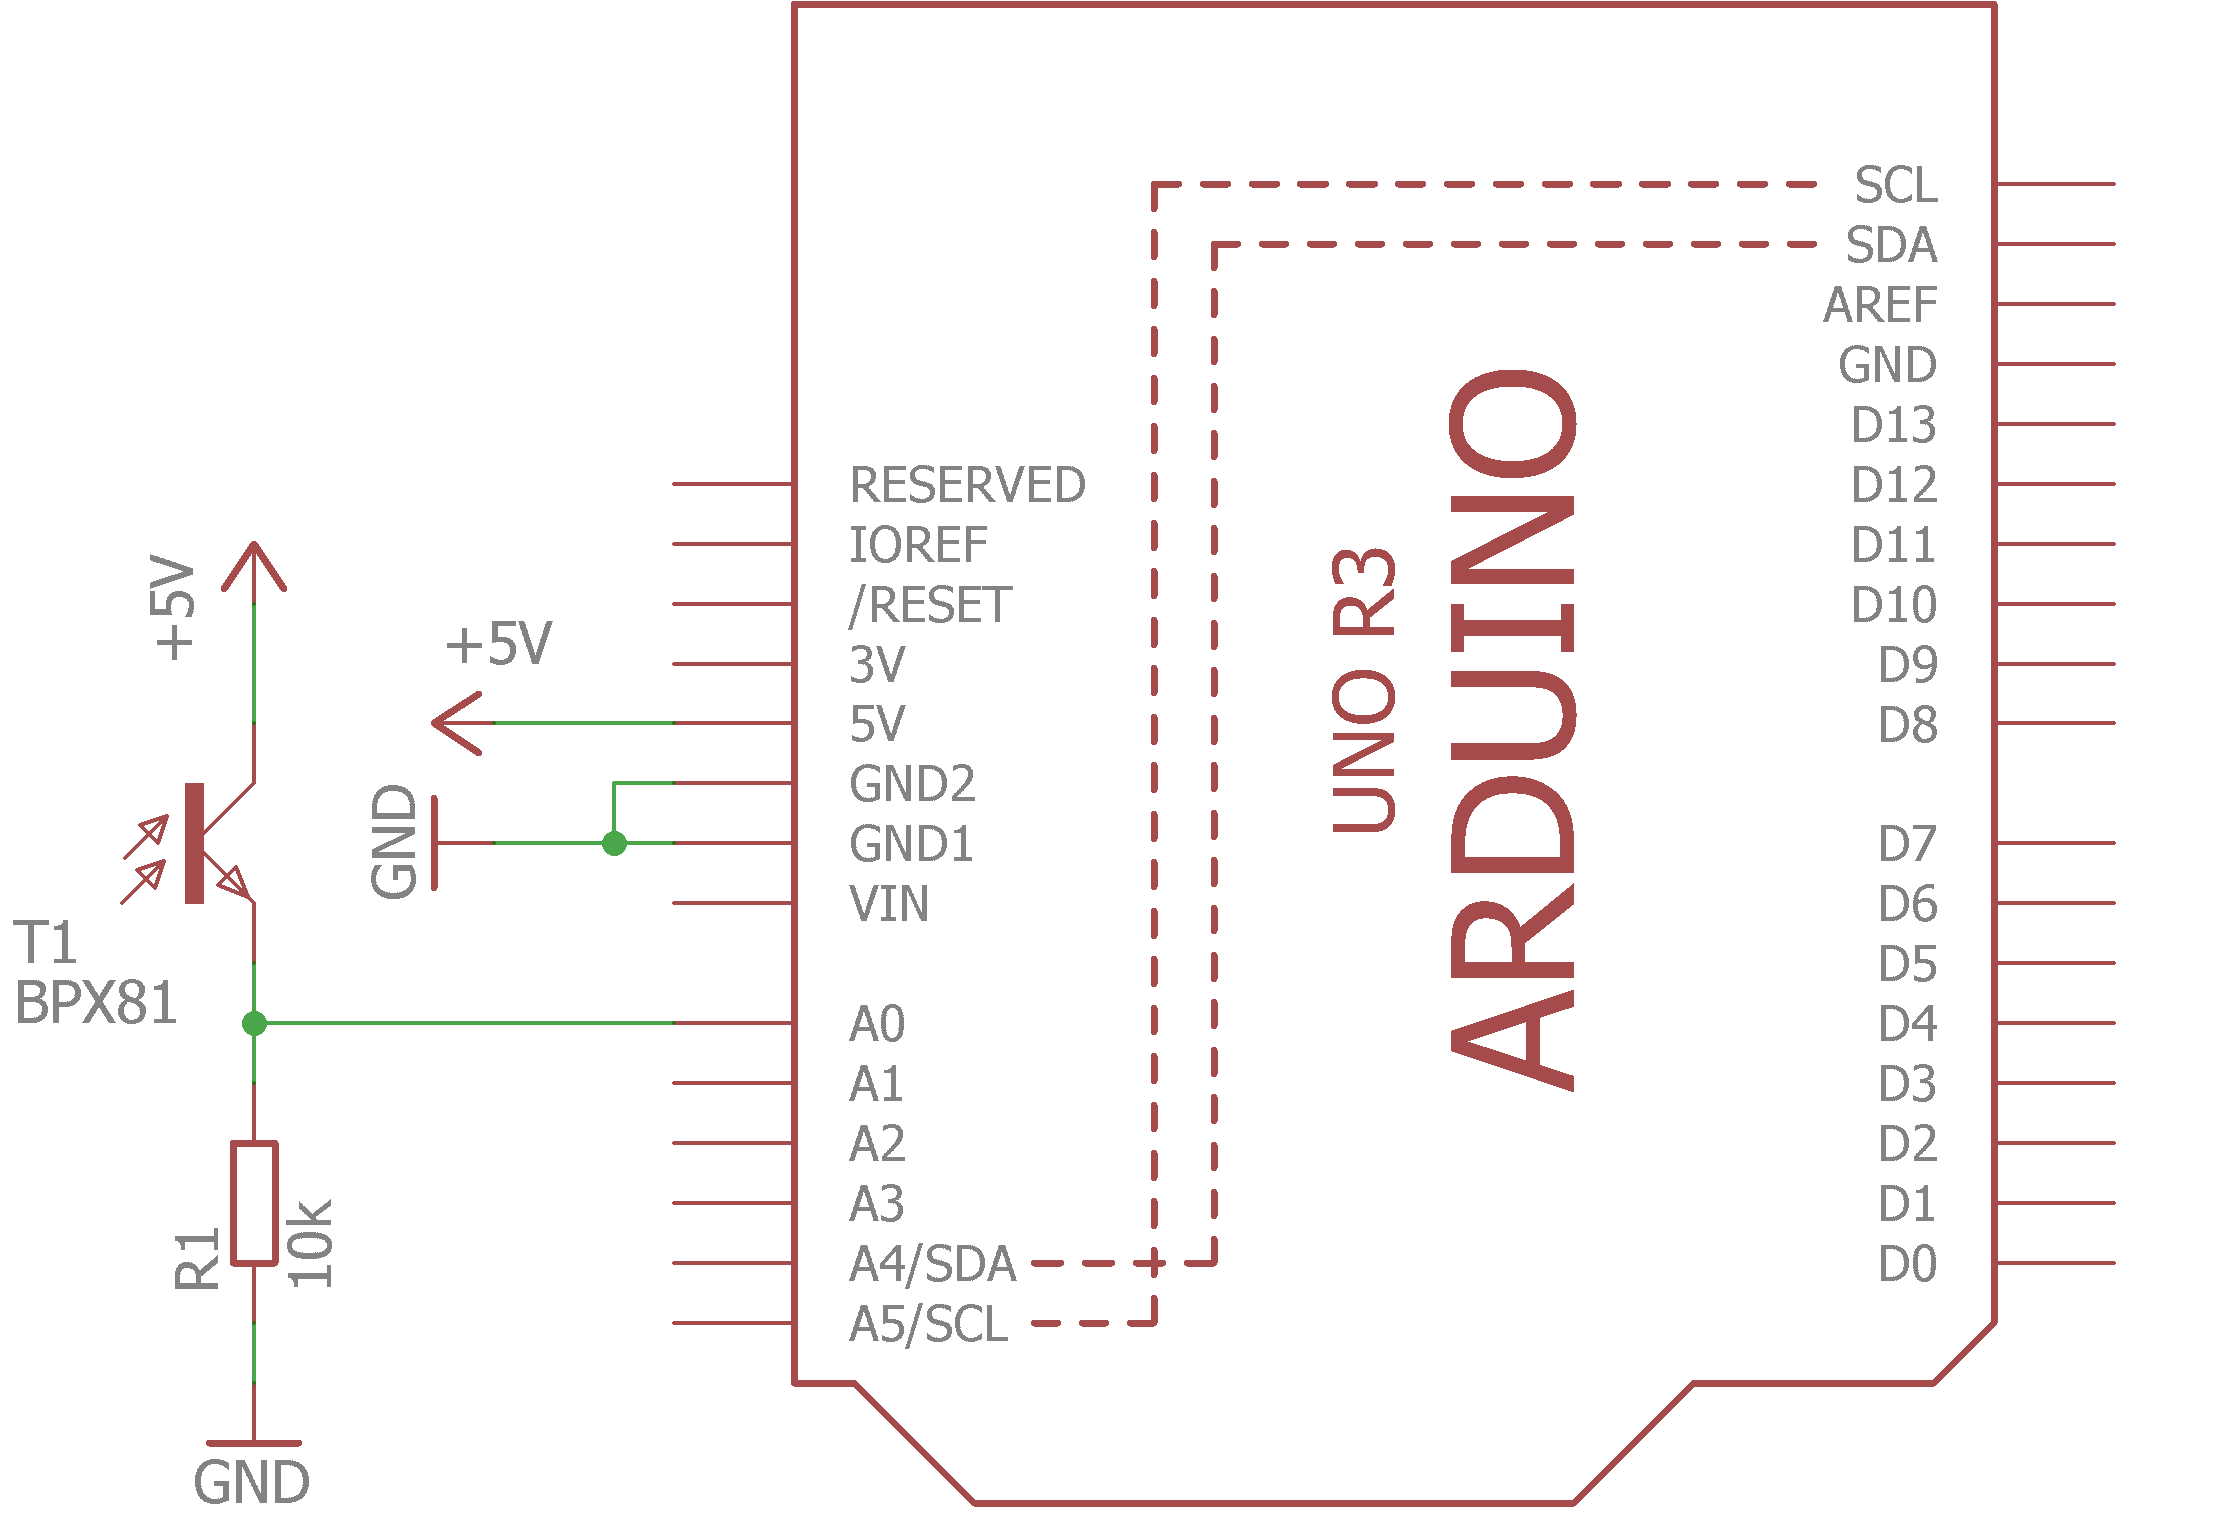
\includegraphics[width=250px]{images/measuring-arduino-system_schema.png}	
	\caption[Schéma zapojení měřicího systému]{Schéma zapojení měřicího systému}
	\label{fig:arduino-measuring-system}
\end{figure}

Jelikož se druhá varianta zdála vhodnější, otestoval jsem ji s~programem, prezentovaným výše, s~danou měřicí sestavou a~osciloskopem. 

\begin{figure}[h]
	\centering
	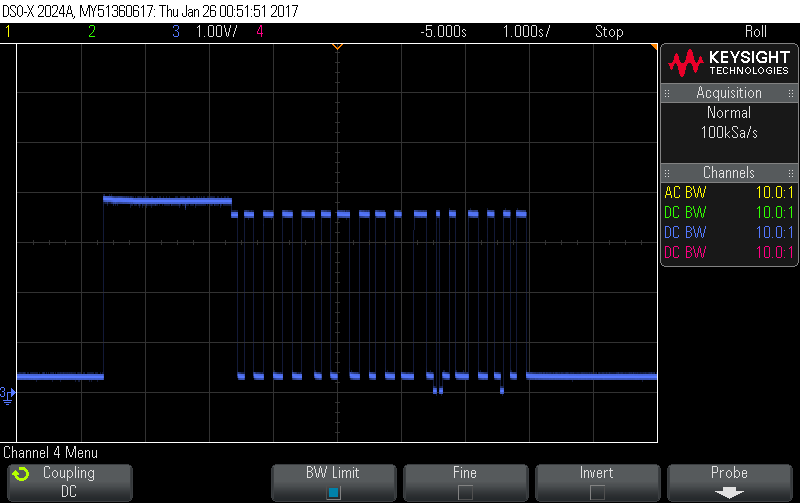
\includegraphics[width=350px]{images/measuring-oscilloscope_ev3-software_led-blinking_all.png}
	\caption[Záznam signálu z~osciloskopu po provedení zkušebního programu]{Záznam signálu z~osciloskopu po provedení zkušebního programu}
	\label{fig:measuring_lego-ev3_orig-soft_led-blinking_all}
\end{figure}

Výsledky byly velice překvapivé. Celkový počet pulzů červené LED (napětí na osciloskopu přibližně 3,7~V; pro zelenou 0,3~V; oranžová 3,9~V) byl 17 
(viz obrázek~\ref{fig:measuring_lego-ev3_orig-soft_led-blinking_all}). Přičemž dle programu mělo proběhnout 200~pulzů.  

Při detailním zkoumání se ukázalo, že LED nedokáží blikat na 50~Hz, ale mohou svůj stav měnit vždy s~frekvencí 20~Hz. 
Každých 50~ms docházelo ke kontrole stavových proměnných u~LED a~případné změně stavu (viz~obrázek~\ref{fig:measuring_lego-ev3_orig-soft_led-blinking_part1} -- jeden dílek odpovídá 100~ms a~1~V).

Toto chování lze například vysvětlit tak, že v~rámci operačního systému \EVbrick{\it u} je v~určité periodě (přibližně 50~ms) vyvoláno přerušení od časovače, které porovná stav proměnných a~registrů LED a~dle výsledku buď rozsvítí, nebo zhasne. 
Proto v~daných intervalech dochází k~interferenci mezi časováním LED (20~ms) a~interního přerušení (přibližně 50~ms) a~podle toho, jak se tyto události sejdou, se jednotlivé LED přepínají.
Tento časovač bude pravděpodobně fungovat jen pro LED, ale nebude dále ovlivňovat další chování systému.
 
\begin{figure}[h]
	\centering
	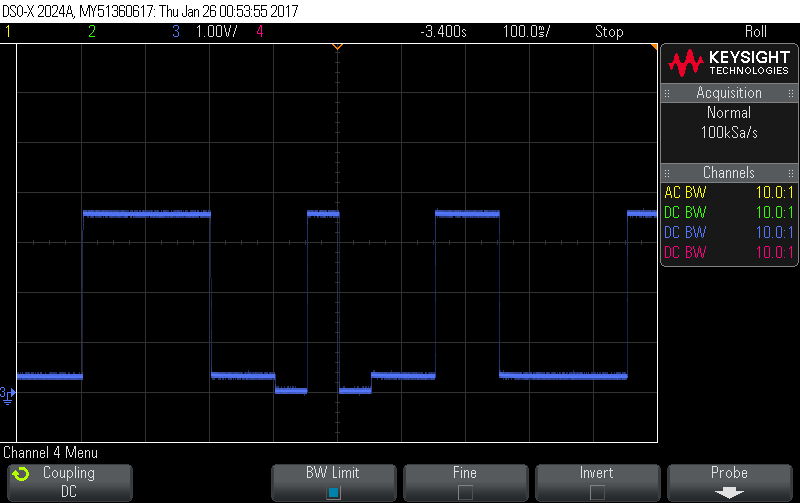
\includegraphics[width=350px]{images/measuring-oscilloscope_ev3-software_led-blinking_part1.png}
	\caption[Zoom na záznam z~osciloskopu po provedení zkušebního programu]{Zoom na záznam z~osciloskopu po provedení zkušebního programu}
	\label{fig:measuring_lego-ev3_orig-soft_led-blinking_part1}
\end{figure}

\begin{figure}[h]
	\centering
	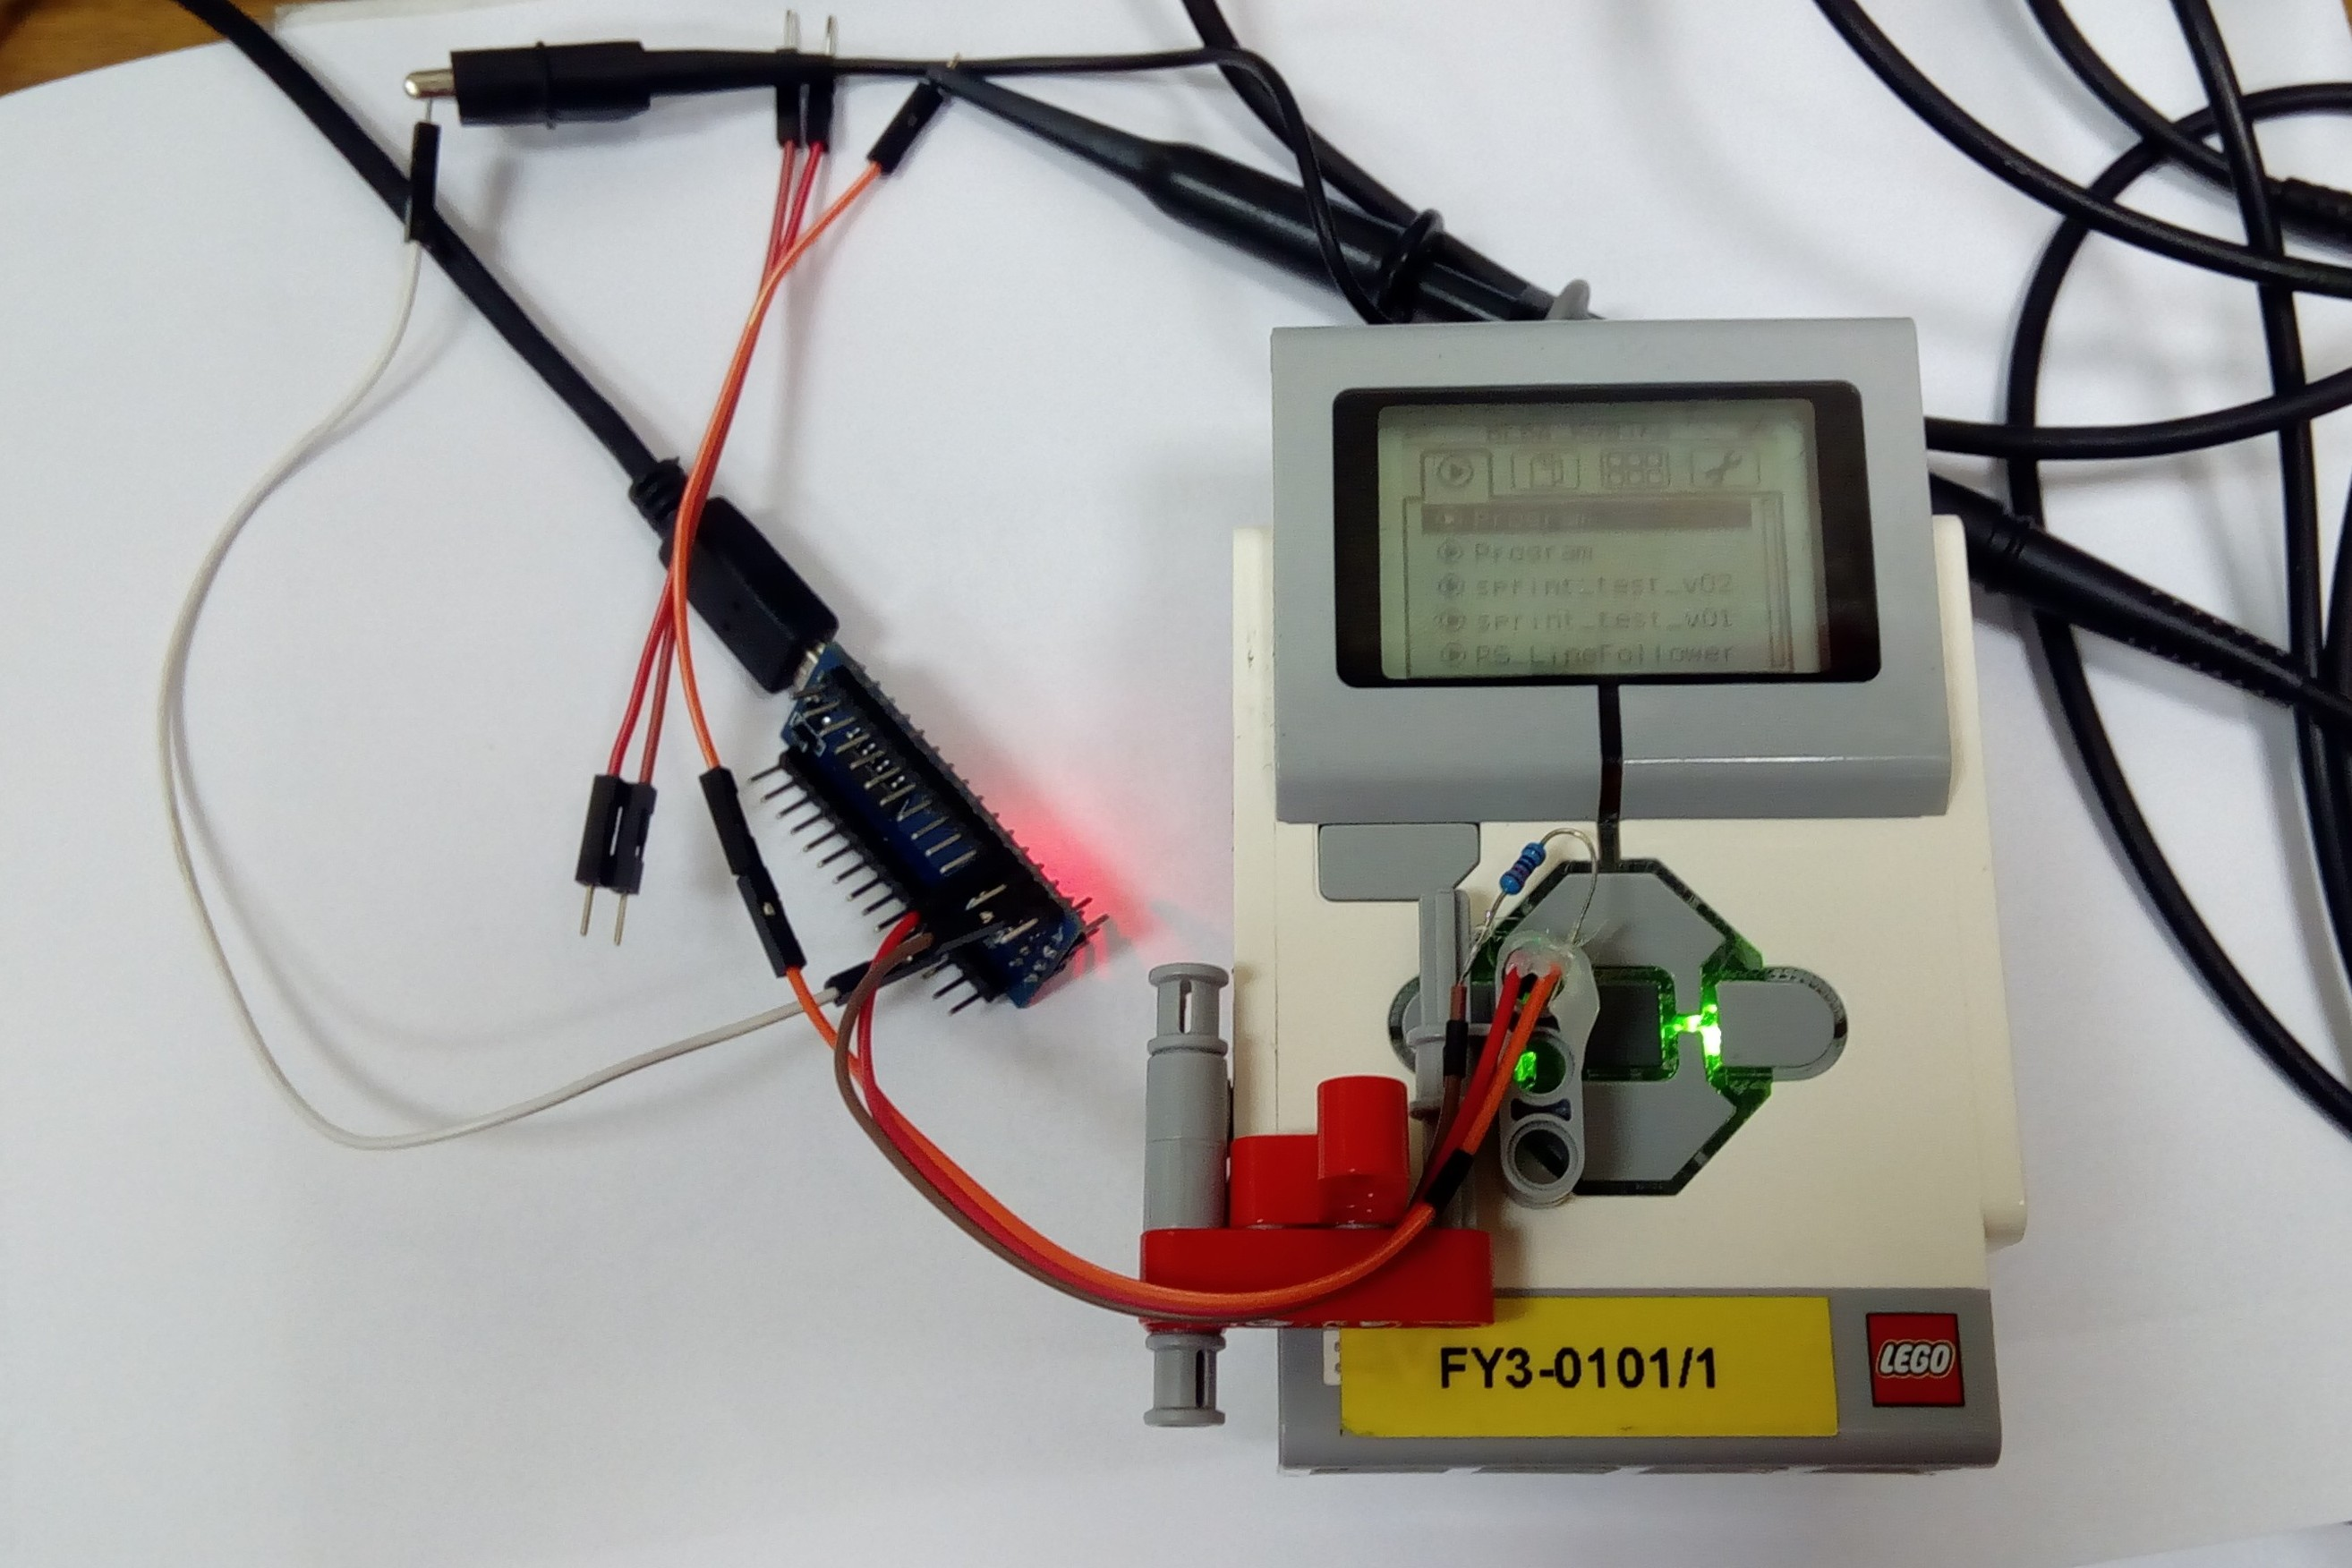
\includegraphics[width=280px]{images/measuring-system_photo.jpg}
	\caption[Foto měřicí sestavy]{Foto měřicí sestavy}
	\label{fig:measuring-system_photo}
\end{figure}

Z~naměřených výsledků vyplývá, že tuto formu testování nelze použít.

\section{Měření jednotlivých operací}

Jelikož nebyli výsledky z~prvního testování uspokojivé, rozhodl jsem se provést testy výkonosti jednotlivých operací na standardním LEGO systému a~RTOS EV3RT (popis v~kapitole \ref{lego-EV3RT}), který dle předchozího zkoumání měl předpoklady k~nejlepšímu výkonu.  \\

V~rámci testů byla vytvořeny dvě sady: 

\begin{itemize}
    \item matematických operací (sčítání, násobení, dělení, \dots) a~podmínka
    \item operace se senzory a~motory
\end{itemize}

Jednotlivé měření se prováděli vícenásobným voláním daných metod (v~rozmezí od~1 do~100~000 volání v~závislosti na době trvání dané operace) tak, aby bylo možné změřit čas s~rozumnou přesností.
Každé měření pak bylo zopakováno 1000, aby bylo možné určit průměr a~maxima. 
Zdrojové soubory k~testům (jak LEGO, tak EV3RT) jsou k~dispozici v~repozitáři RB-ev3rt-hrp2-sdk~\cite{RB-ev3rt-hrp2-sdk-github}.

Matematické operace, jako sčítání, násobení, dělení byly prováděny v~plovoucí desetinné čárce (double).

Z~výkonnostních testu (tabulka~\ref{Benchmark-math} a~\ref{Benchmark-IO}) je dobře vidět, že zpracování operací probíhá na systému EV3RT více jak o~2~řády rychlejší než u~oficiálního systému \EVthree{}. Proto jsem vybral tento systém jako nejvhodnější variantu pro  vytvoření vývojové prostředí.

\begin{table}[h]
\centering

\caption{Porovnání relativního výpočetního výkonu originálního LEGO systému a~EV3RT -- matematické operace a~podmínka \\
}

\label{Benchmark-math}
\begin{tabular}{@{}ccrrr@{}}
\toprule
Označení testu                                       & AVG/MAX                     & LEGO                               & EV3RT                                & Porovnání                                                    \\ \midrule
\multicolumn{1}{|c}{}                                & \cellcolor[HTML]{EFEFEF}AVG & \cellcolor[HTML]{EFEFEF}    563 us & \cellcolor[HTML]{EFEFEF}    0.586 us & \multicolumn{1}{r|}{\cellcolor[HTML]{EFEFEF}    960 $\times$}  \\
\multicolumn{1}{|c}{\multirow{-2}{*}{sčítání}}           & \cellcolor[HTML]{FFFFFF}MAX & \cellcolor[HTML]{FFFFFF}    680 us & \cellcolor[HTML]{FFFFFF}    0.602 us & \multicolumn{1}{r|}{\cellcolor[HTML]{FFFFFF}   1129 $\times$}  \\ \midrule
\multicolumn{1}{|c}{}                                & \cellcolor[HTML]{EFEFEF}AVG & \cellcolor[HTML]{EFEFEF}    388 us & \cellcolor[HTML]{EFEFEF}    0.506 us & \multicolumn{1}{r|}{\cellcolor[HTML]{EFEFEF}    766 $\times$}  \\
\multicolumn{1}{|c}{\multirow{-2}{*}{násobení}}          & \cellcolor[HTML]{FFFFFF}MAX & \cellcolor[HTML]{FFFFFF}    510 us & \cellcolor[HTML]{FFFFFF}    0.526 us & \multicolumn{1}{r|}{\cellcolor[HTML]{FFFFFF}    969 $\times$}  \\ \midrule
\multicolumn{1}{|c}{}                                & \cellcolor[HTML]{EFEFEF}AVG & \cellcolor[HTML]{EFEFEF}    403 us & \cellcolor[HTML]{EFEFEF}    2.627 us & \multicolumn{1}{r|}{\cellcolor[HTML]{EFEFEF}    153 $\times$}  \\
\multicolumn{1}{|c}{\multirow{-2}{*}{dělení}}           & \cellcolor[HTML]{FFFFFF}MAX & \cellcolor[HTML]{FFFFFF}    510 us & \cellcolor[HTML]{FFFFFF}    2.943 us & \multicolumn{1}{r|}{\cellcolor[HTML]{FFFFFF}    173 $\times$}  \\ \midrule
\multicolumn{1}{|c}{}                                & \cellcolor[HTML]{EFEFEF}AVG & \cellcolor[HTML]{EFEFEF}    557 us & \cellcolor[HTML]{EFEFEF}   43.350 us & \multicolumn{1}{r|}{\cellcolor[HTML]{EFEFEF}     12 $\times$}  \\
\multicolumn{1}{|c}{\multirow{-2}{*}{mocnina}}           & \cellcolor[HTML]{FFFFFF}MAX & \cellcolor[HTML]{FFFFFF}   1480 us & \cellcolor[HTML]{FFFFFF}   47.860 us & \multicolumn{1}{r|}{\cellcolor[HTML]{FFFFFF}     30 $\times$}  \\ \midrule
\multicolumn{1}{|c}{}                                & \cellcolor[HTML]{EFEFEF}AVG & \cellcolor[HTML]{EFEFEF}    488 us & \cellcolor[HTML]{EFEFEF}    5.250 us & \multicolumn{1}{r|}{\cellcolor[HTML]{EFEFEF}     92 $\times$}  \\
\multicolumn{1}{|c}{\multirow{-2}{*}{odmocnina}}          & \cellcolor[HTML]{FFFFFF}MAX & \cellcolor[HTML]{FFFFFF}    890 us & \cellcolor[HTML]{FFFFFF}    6.146 us & \multicolumn{1}{r|}{\cellcolor[HTML]{FFFFFF}    144 $\times$}  \\ \midrule
\multicolumn{1}{|c}{}                                & \cellcolor[HTML]{EFEFEF}AVG & \cellcolor[HTML]{EFEFEF}    411 us & \cellcolor[HTML]{EFEFEF}   12.520 us & \multicolumn{1}{r|}{\cellcolor[HTML]{EFEFEF}     32 $\times$}  \\
\multicolumn{1}{|c}{\multirow{-2}{*}{sinus}}           & \cellcolor[HTML]{FFFFFF}MAX & \cellcolor[HTML]{FFFFFF}    590 us & \cellcolor[HTML]{FFFFFF}   15.780 us & \multicolumn{1}{r|}{\cellcolor[HTML]{FFFFFF}     37 $\times$}  \\ \midrule
\multicolumn{1}{|c}{}                                & \cellcolor[HTML]{EFEFEF}AVG & \cellcolor[HTML]{EFEFEF}    419 us & \cellcolor[HTML]{EFEFEF}    0.126 us & \multicolumn{1}{r|}{\cellcolor[HTML]{EFEFEF}   3325 $\times$}  \\
\multicolumn{1}{|c}{\multirow{-2}{*}{podmínka}}     & \cellcolor[HTML]{FFFFFF}MAX & \cellcolor[HTML]{FFFFFF}    510 us & \cellcolor[HTML]{FFFFFF}    0.139 us & \multicolumn{1}{r|}{\cellcolor[HTML]{FFFFFF}   3669 $\times$}  \\ \midrule
\end{tabular}
\end{table}

\begin{table}[]
\centering
\caption{Porovnání relativního výpočetního výkonu originálního LEGO systému a~EV3RT -- \brick{} komponenty, motory a~senzory}
\label{Benchmark-IO}
\begin{tabular}{@{}ccrrr@{}}
\toprule
Označení testu                                       & AVG/MAX                     & LEGO                               & EV3RT                                & Porovnání                                                    \\ \midrule
\multicolumn{1}{|c}{}                                & \cellcolor[HTML]{EFEFEF}AVG & \cellcolor[HTML]{EFEFEF}    966 us & \cellcolor[HTML]{EFEFEF}    0.350 us & \multicolumn{1}{r|}{\cellcolor[HTML]{EFEFEF}   2760 $\times$}  \\
\multicolumn{1}{|c}{\multirow{-2}{*}{brick button}}  & \cellcolor[HTML]{FFFFFF}MAX & \cellcolor[HTML]{FFFFFF}   1100 us & \cellcolor[HTML]{FFFFFF}    0.362 us & \multicolumn{1}{r|}{\cellcolor[HTML]{FFFFFF}   3038 $\times$}  \\ \midrule
\multicolumn{1}{|c}{}                                & \cellcolor[HTML]{EFEFEF}AVG & \cellcolor[HTML]{EFEFEF}    787 us & \cellcolor[HTML]{EFEFEF}    2.866 us & \multicolumn{1}{r|}{\cellcolor[HTML]{EFEFEF}    274 $\times$}  \\
\multicolumn{1}{|c}{\multirow{-2}{*}{brick led}}     & \cellcolor[HTML]{FFFFFF}MAX & \cellcolor[HTML]{FFFFFF}    900 us & \cellcolor[HTML]{FFFFFF}    3.247 us & \multicolumn{1}{r|}{\cellcolor[HTML]{FFFFFF}    277 $\times$}  \\ \midrule
\multicolumn{1}{|c}{}                                & \cellcolor[HTML]{EFEFEF}AVG & \cellcolor[HTML]{EFEFEF}   1449 us & \cellcolor[HTML]{EFEFEF}  396.080 us & \multicolumn{1}{r|}{\cellcolor[HTML]{EFEFEF}      3 $\times$}  \\
\multicolumn{1}{|c}{\multirow{-2}{*}{brick display}} & \cellcolor[HTML]{FFFFFF}MAX & \cellcolor[HTML]{FFFFFF}   1620 us & \cellcolor[HTML]{FFFFFF}  409.330 us & \multicolumn{1}{r|}{\cellcolor[HTML]{FFFFFF}      3 $\times$}  \\ \midrule
\multicolumn{1}{|c}{}                                & \cellcolor[HTML]{EFEFEF}AVG & \cellcolor[HTML]{EFEFEF}    603 us & \cellcolor[HTML]{EFEFEF}    8.770 us & \multicolumn{1}{r|}{\cellcolor[HTML]{EFEFEF}     68 $\times$}  \\
\multicolumn{1}{|c}{\multirow{-2}{*}{motor power}}   & \cellcolor[HTML]{FFFFFF}MAX & \cellcolor[HTML]{FFFFFF}    720 us & \cellcolor[HTML]{FFFFFF}   11.630 us & \multicolumn{1}{r|}{\cellcolor[HTML]{FFFFFF}     61 $\times$}  \\ \midrule
\multicolumn{1}{|c}{}                                & \cellcolor[HTML]{EFEFEF}AVG & \cellcolor[HTML]{EFEFEF}    612 us & \cellcolor[HTML]{EFEFEF}    8.840 us & \multicolumn{1}{r|}{\cellcolor[HTML]{EFEFEF}     69 $\times$}  \\
\multicolumn{1}{|c}{\multirow{-2}{*}{motor speed}}   & \cellcolor[HTML]{FFFFFF}MAX & \cellcolor[HTML]{FFFFFF}    760 us & \cellcolor[HTML]{FFFFFF}   11.670 us & \multicolumn{1}{r|}{\cellcolor[HTML]{FFFFFF}     65 $\times$}  \\ \midrule
\multicolumn{1}{|c}{}                                & \cellcolor[HTML]{EFEFEF}AVG & \cellcolor[HTML]{EFEFEF}   1023 us & \cellcolor[HTML]{EFEFEF}   17.490 us & \multicolumn{1}{r|}{\cellcolor[HTML]{EFEFEF}     58 $\times$}  \\
\multicolumn{1}{|c}{\multirow{-2}{*}{motors speed}}  & \cellcolor[HTML]{FFFFFF}MAX & \cellcolor[HTML]{FFFFFF}   1160 us & \cellcolor[HTML]{FFFFFF}   21.120 us & \multicolumn{1}{r|}{\cellcolor[HTML]{FFFFFF}     54 $\times$}  \\ \midrule
\multicolumn{1}{|c}{}                                & \cellcolor[HTML]{EFEFEF}AVG & \cellcolor[HTML]{EFEFEF}    785 us & \cellcolor[HTML]{EFEFEF}    3.870 us & \multicolumn{1}{r|}{\cellcolor[HTML]{EFEFEF}    202 $\times$}  \\
\multicolumn{1}{|c}{\multirow{-2}{*}{CS reflected}}  & \cellcolor[HTML]{FFFFFF}MAX & \cellcolor[HTML]{FFFFFF}    940 us & \cellcolor[HTML]{FFFFFF}    6.980 us & \multicolumn{1}{r|}{\cellcolor[HTML]{FFFFFF}    134 $\times$}  \\ \midrule
\multicolumn{1}{|c}{}                                & \cellcolor[HTML]{EFEFEF}AVG & \cellcolor[HTML]{EFEFEF}    830 us & \cellcolor[HTML]{EFEFEF}    3.860 us & \multicolumn{1}{r|}{\cellcolor[HTML]{EFEFEF}    215 $\times$}  \\
\multicolumn{1}{|c}{\multirow{-2}{*}{CS ambient}}    & \cellcolor[HTML]{FFFFFF}MAX & \cellcolor[HTML]{FFFFFF}    990 us & \cellcolor[HTML]{FFFFFF}    7.100 us & \multicolumn{1}{r|}{\cellcolor[HTML]{FFFFFF}    139 $\times$}  \\ \midrule
\multicolumn{1}{|c}{}                                & \cellcolor[HTML]{EFEFEF}AVG & \cellcolor[HTML]{EFEFEF}    799 us & \cellcolor[HTML]{EFEFEF}    3.890 us & \multicolumn{1}{r|}{\cellcolor[HTML]{EFEFEF}    205 $\times$}  \\
\multicolumn{1}{|c}{\multirow{-2}{*}{CS color}}      & \cellcolor[HTML]{FFFFFF}MAX & \cellcolor[HTML]{FFFFFF}    930 us & \cellcolor[HTML]{FFFFFF}    6.730 us & \multicolumn{1}{r|}{\cellcolor[HTML]{FFFFFF}    138 $\times$}  \\ \midrule
\multicolumn{1}{|c}{}                                & \cellcolor[HTML]{EFEFEF}AVG & \cellcolor[HTML]{EFEFEF}    811 us & \cellcolor[HTML]{EFEFEF}    3.841 us & \multicolumn{1}{r|}{\cellcolor[HTML]{EFEFEF}    211 $\times$}  \\
\multicolumn{1}{|c}{\multirow{-2}{*}{UTS cm}}        & \cellcolor[HTML]{FFFFFF}MAX & \cellcolor[HTML]{FFFFFF}    960 us & \cellcolor[HTML]{FFFFFF}    4.212 us & \multicolumn{1}{r|}{\cellcolor[HTML]{FFFFFF}    227 $\times$}  \\ \midrule
\multicolumn{1}{|c}{}                                & \cellcolor[HTML]{EFEFEF}AVG & \cellcolor[HTML]{EFEFEF}    827 us & \cellcolor[HTML]{EFEFEF}    3.838 us & \multicolumn{1}{r|}{\cellcolor[HTML]{EFEFEF}    215 $\times$}  \\
\multicolumn{1}{|c}{\multirow{-2}{*}{UTS inch}}      & \cellcolor[HTML]{FFFFFF}MAX & \cellcolor[HTML]{FFFFFF}   1030 us & \cellcolor[HTML]{FFFFFF}    4.197 us & \multicolumn{1}{r|}{\cellcolor[HTML]{FFFFFF}    245 $\times$}  \\ \midrule
\multicolumn{1}{|c}{}                                & \cellcolor[HTML]{EFEFEF}AVG & \cellcolor[HTML]{EFEFEF}    845 us & \cellcolor[HTML]{EFEFEF}    3.769 us & \multicolumn{1}{r|}{\cellcolor[HTML]{EFEFEF}    224 $\times$}  \\
\multicolumn{1}{|c}{\multirow{-2}{*}{UTS listen}}    & \cellcolor[HTML]{FFFFFF}MAX & \cellcolor[HTML]{FFFFFF}   1220 us & \cellcolor[HTML]{FFFFFF}    4.115 us & \multicolumn{1}{r|}{\cellcolor[HTML]{FFFFFF}    296 $\times$}  \\ \midrule
\multicolumn{1}{|c}{}                                & \cellcolor[HTML]{EFEFEF}AVG & \cellcolor[HTML]{EFEFEF}    851 us & \cellcolor[HTML]{EFEFEF}    3.910 us & \multicolumn{1}{r|}{\cellcolor[HTML]{EFEFEF}    217 $\times$}  \\
\multicolumn{1}{|c}{\multirow{-2}{*}{GYRO angle}}    & \cellcolor[HTML]{FFFFFF}MAX & \cellcolor[HTML]{FFFFFF}   1050 us & \cellcolor[HTML]{FFFFFF}    6.740 us & \multicolumn{1}{r|}{\cellcolor[HTML]{FFFFFF}    155 $\times$}  \\ \midrule
\multicolumn{1}{|c}{}                                & \cellcolor[HTML]{EFEFEF}AVG & \cellcolor[HTML]{EFEFEF}    847 us & \cellcolor[HTML]{EFEFEF}    3.920 us & \multicolumn{1}{r|}{\cellcolor[HTML]{EFEFEF}    216 $\times$}  \\
\multicolumn{1}{|c}{\multirow{-2}{*}{GYRO rate}}     & \cellcolor[HTML]{FFFFFF}MAX & \cellcolor[HTML]{FFFFFF}   1250 us & \cellcolor[HTML]{FFFFFF}    7.190 us & \multicolumn{1}{r|}{\cellcolor[HTML]{FFFFFF}    173 $\times$}  \\ \midrule
\multicolumn{1}{|c}{}                                & \cellcolor[HTML]{EFEFEF}AVG & \cellcolor[HTML]{EFEFEF}  25712 us & \cellcolor[HTML]{EFEFEF}    3.510 us & \multicolumn{1}{r|}{\cellcolor[HTML]{EFEFEF}   7325 $\times$}  \\
\multicolumn{1}{|c}{\multirow{-2}{*}{GYRO reset}}    & \cellcolor[HTML]{FFFFFF}MAX & \cellcolor[HTML]{FFFFFF}  34410 us & \cellcolor[HTML]{FFFFFF}    6.420 us & \multicolumn{1}{r|}{\cellcolor[HTML]{FFFFFF}   5359 $\times$}  \\ \midrule
\end{tabular}
\end{table}


  
  \chapter{Vývojová platforma}

Poté, co jsem si udělal přehled všech existujících platforem pro \legoEV{} v~rámci kapitoly~\ref{lego-soft-available-platforms}, a provedl testování výkonu v~kapitole~\ref{testing} jsem pro svou práci vybral prostředí EV3RT.
Nad touto platformou jsem se rozhodl vybudovat vývojové prostředí vhodné pro začátečníky a~stanovil jsem si následující požadavky:

\begin{itemize}
\item C++~API blízké programovacím blokům v~\lego{} prostředí s~anglickou dokumentací
\item průvodce práce s~vývojovou platformou v~češtině
\item modul pro správu EV3 portů (obdoba informačního panelu s~porty v~EV3 prostředí)  
\item předpřipravená obsluha komunikace a~práce se soubory
\item snadné ovládání základních periferií na EV3 (displej, LED, tlačítka)
\item vývojářské IDE\footnote{IDE = Integrated Development Environment} s~jednoduchým rozhraním a~našeptáváním 
\item zautomatizovaný build proces a~nahrávání programů do \brick{\it u}
\item jednoduchá instalace u~uživatele
\end{itemize}
V~následujících podkapitolách se budu podrobněji věnovat jednotlivým bodům.


\section{Vývojový proces při rozšiřování EV3RT}

Při vývoji a~rozšiřování systému EV3RT jsem chtěl využít všech běžných vývojářských nástrojů a~služeb.
Prioritou bylo verzování, bez kterého se dnes prakticky žádný dlouhodobější projekt neobejde. Díky tomu lze na projektech snadno spolupracovat s~lidmi po celém světě.
Jelikož EV3RT již mělo svůj repozitář na GitHubu~\cite{legoProgramingPlatform_EV3RT-github}, neměl jsem důvod přemýšlet nad jinou službou.
Celý projekt vyvíjím jako forky původních repozitářů. Mohu tak jednoduše vyvíjet pro EV3RT a~zasílat pull-requesty autorům s~případnými opravami nebo vylepšeními.
Repozitář RB-ev3rt-hrp2~\cite{RB-ev3rt-hrp2-github} obsahuje kompletní systém EV3RT (RTOS TOPPERS/HRP2, drivery pro \brick{}, \dots). 

V~repozitáři RB-ev3rt-hrp2-sdk~\cite{RB-ev3rt-hrp2-sdk-github} je workspace pro aplikace a~knihovny s~API pro EV3 (nachází se zde kompletní implementace C++ API). RB-ev3rt-hrp2-sdk je v~podobě subrepozitáře distribuován i~v~RB-ev3rt-hrp2. Repozitáře jsou na GitHubu uloženy pod komunitou RobotikaBrno~\cite{RobotikaBrno-web}, na jejímž chodu se ve volném čase podílím. Proto také mají i~všechny repozitáře předponu RB~\cite{RoboticsBrno-github}. RobotikaBrno má za cíl podporu robotiky v~Brně a~České republice.

V~rámci testovaní a~integrace se systémem EV3RT jsem použil CI\footnote{CI = Continuous Integration} na serveru Travis~\cite{Travis-web}.
Tato služba má velmi dobré propojení s~GitHubem. 
CI po každém commitu spouští kompilaci nad jednotlivými testovacími projekty.
Aktuálně tak provádím základní testování přeložitelnosti kódu~\cite{Travis-RB-ev3rt-hrp2-sdk}.
Díky tomu mohu zachytit nekonzistentnost na různých místech API, ověřit kompatibilitu s~EV3RT a~zkontrolovat zkompilovatelnost pro všechny vzorové projekty.  
Jelikož je celý systém EV3RT hardwarově závislý na \legoEV{}, finální testování provádím spouštěním předpřipravených testovacích projektů na reálném hardwaru.

Když jsem přemýšlel nad tím, jak by nejlépe mělo vypadat programovací API pro \lego{}, došel jsem po různých pokusech a~diskuzích se studenty k~závěru, že pro začátečníka bude nejvhodnější objektově orientované API.
Pro začínajícího programátora je dle mého mínění objektová abstrakce přirozená z~reálného světa a~proto se mu s~objekty bude lépe pracovat.
Zároveň zapouzdřenost objektů odstiňuje uživatele od implementace a~tím jej méně rozptyluje od jeho záměru a~cíle.

\subsection{EV3RT C API}


Předtím, než jsem začal tvořit vlastní C++~API, jsem si důkladně nastudoval a~vyzkoušel EV3RT C~API, abych měl jasnou představu, jak vše funguje.
Dokumentace byla tvořena v~Doxygenu~\cite{doxygen-web}, a~tak jsem se rozhodl ji rozšířit za pomocí Google Translate a~vlastní intuice o anglický překlad.
Doxygen je jeden z~nejpoužívanějších nástrojů na tvorbu dokumentace k softwarovým projektům. 
Zvládá generovat jak webové stránky, tak PDF dokumenty pro offline použití.

Po přeložení všech knihoven jsem přes GitHub Pages vytvořil online verzi dokumentace~\cite{roboticsbrno-EV3RT-API-Reference}.
Zároveň jsem zaslal pull-request autorům EV3RT, kteří jej přijali a~na svých webových stránkách odkazují na mnou vytvořenou dokumentaci~\cite{EV3RT-git-web_documentation}.

\subsection{EV3RT C++ API}


Pro EV3RT již existovalo základní C++~API~\cite{EV3RT-git-web_documentation}, vytvořené v~rámci projektu ETrobocon/etroboEV3~\cite{ev3rt-cpp-API-ETrobocon}. Z~následujících důvodů jsem se jej rozhodl nevyužít:
 
\begin{itemize}
    \item nebylo součástí oficiálních EV3RT repozitářů
    \item autoři EV3RT jej nepovažují za oficiální API a~nejedná se o~jejich výtvor
    \item implementovány jen některé funkce a~dokumentace v~japonštině
    \item rozdílná představa o~implementaci některých části API     
\end{itemize}

\subsection{C++ API}

Při procházení C~API v~EV3RT jsem nebyl spokojen s~jeho použitím pro začátečníky. 
API~sice umožňuje přímý přístup k~hardwaru, tím ale uživateli poskytuje větší prostor k~chybám a~tomu
 je potřeba předcházet. 
V~C++~API těmto věcem předcházím pomocí různých prostředků: konstrukcí jazyka (např.~\texttt{enum class}, defaultní parametry funkcí, přetěžováním konstruktorů), názvy funkcí nebo pojmenováním parametrů či~výčtových typů.

Pro srovnání jsem připravil ukázku C~API (obrázek~\ref{src:ev3api-triangle}) a~svého C++~API (obrázek~\ref{src:ev3cxx-triangle}). 
Na ukázkách je program pro objetí trojúhelníku. V~C~API není k dispozici funkce, která by umožňovala řídit oba motory naráz, proto se implementace lehce liší.


\begin{figure}[H] 
    \begin{minted}[linenos=false]{cpp}
ev3_motor_rotate(motor_port_t port, int degrees, 
                 uint32_t speed_abs, bool_t blocking)
    \end{minted}
    \caption{Prototypy C API funkce pro nastaveni ujeté vzdálenosti na jednom motoru}
    \label{src:ev3api_motor-rotate}
\end{figure}

\begin{figure}[H] 
    \begin{minted}[xleftmargin=1.5em,linenos=true]{cpp}
void main_task(intptr_t unused) {   
    ev3_motor_rotate(EV3_PORT_B, 360, 50, false);
    ev3_motor_rotate(EV3_PORT_C, 360, 50, true);
    ev3_motor_rotate(EV3_PORT_B, 520, 50, true);
    
    ev3_motor_rotate(EV3_PORT_B, 360, 50, false);
    ev3_motor_rotate(EV3_PORT_C, 360, 50, true);
    ev3_motor_rotate(EV3_PORT_B, 520, 50, true);
    
    ev3_motor_rotate(EV3_PORT_B, 360, 50, false);
    ev3_motor_rotate(EV3_PORT_C, 360, 50, true);
    ev3_motor_rotate(EV3_PORT_B, 520, 50, true);
}
    \end{minted}
    \caption[Ukázka kódu pro objetí trojúhelníku v~C~API]{
    Ukázka kódu pro objetí trojúhelníku v~C~API \\
    Uživatel musí použít několikrát příkaz pro nastavení otočení motorů se správně zadaným portem (EV3\_PORT\_B/EV3\_PORT\_C) a~parametry. 
    Může zde jednoduše dojít k~přepsání se u~označení portu, požadovaného úhlu otočení nebo u parametru blokování -- vykonávání programu je pozastaveno do doby, než motor dojede na požadovanou pozici. 

    }
    \label{src:ev3api-triangle}
\end{figure}

\begin{figure}[H] 
    \begin{minted}[linenos=false]{cpp}
MotorTank::onForDegrees(int left_speed = 50, int right_speed = 50, 
                        int degrees = 360, bool_t brake = true, 
                        bool_t blocking = true, 
                        unsigned int wait_after_ms = 60);
    \end{minted}
    \caption[Prototypy C++ API funkce pro nastaveni ujeté vzdálenosti v režimu MotorTank]{Prototypy C++ API funkce pro nastaveni ujeté vzdálenosti v režimu MotorTank (spojení dvou motory)}
    \label{src:ev3cxx_motor-rotate}
\end{figure}
\begin{figure}[H] 
    \begin{minted}[xleftmargin=1.5em,linenos=true]{cpp}
void main_task(intptr_t unused) {    
    ev3cxx::MotorTank motors(ev3cxx::MotorPort::B, ev3cxx::MotorPort::C);   
    
    motors.onForDegrees(50, 50, 360);
    motors.onForDegrees(50,  0, 520);

    motors.onForDegrees(50, 50, 360);
    motors.onForDegrees(50,  0, 520); 

    motors.onForDegrees(50, 50, 360);
    motors.onForDegrees(50,  0, 520);
}
    \end{minted}
    \caption[Ukázka kódu pro objetí trojúhelníku v~mnou navrženém C++~API]{Ukázka kódu pro objetí trojúhelníku v~mnou navrženém C++~API \\
    Uživatel si nejprve vytvoří instanci objektu \texttt{MotorTank} a v~konstruktoru nadefinuje porty, na kterých má motory připojeny. 
    Následně již stačí volat funkci \texttt{onForRotations()} nad instancí \texttt{motors} pro dojetí na konkrétní pozice.    
    }
    \label{src:ev3cxx-triangle}
\end{figure}

\subsection{Implementace}


V~mém C++~API jsem implementoval obsluhu všech komponentů, které EV3RT podporuje (EV3 motory a~senzory, tlačítka, LED, displej a~reproduktor na \brick{\it u}).
Zároveň jsem chtěl usnadnit uživateli práci se soubory, zápis na displej a~komunikace přes Bluetooth, a~proto jsem pro tyto činnosti nachystal  jednotné rozhraní.

API jsem tvořil v~podobě C++~knihoven. 
Zpočátku jsem se domníval, že rozdělení souborů na zdrojové (\texttt{.cpp}) a~hlavičkové (\texttt{.h}) povede k lepší přehlednosti a~rychlejšímu překladu.

Když jsem ale začal používat šablony a~část implementace byla ve~zdrojových a~část v~hlavičkových souborech, začal jsem nad výhodností rozdělení pochybovat.
Při každé změně API bylo nutné udržovat konzistenci obou souborů a~tato činnost zpomalovala vývoj. 
Proto jsem se rozhodl používat jen hlavičkové soubory. Knihovna je relativně malá a předpokládám, že se to na čase překladu výrazně neprojeví.
Dle pozorování to opravdu nemá žádný podstatný vliv.

Jeden zdrojový soubor (\texttt{ev3cxx.cpp}) jsem si ale ponechal. 
Vytvářím v~něm globální instance tříd, které by měl mít uživatel  k dispozici. 
Nechci tedy, aby si uživatel tyto instance vytvářel sám lokálně.

Snažím se tím předejít vícenásobnému vytvoření daných objektů a~následného nežádoucího chování.
Toto řešení jsem zvolil například u~třídy pro obsluhu displeje. Každá instance displeje si udržuje informace o~aktuální poloze kurzoru na displeji a~v~případě vytvoření více instancí by docházelo k~nežádoucímu chování v podobě přepisování textů z jedné instance tou druhou.
Zvažoval jsem i~použití návrhového vzoru singleton~\cite{design-pattern-singleton}, ale nakonec jsem jej zavrhl, protože by uživatel musel používat konstrukci \texttt{getInstance()}, čímž jsem nechtěl začínající uživatele zatěžovat.

Pro snadné používání v~uživatelských projektech jsem se rozhodl jeden hlavičkový soubor (\texttt{ev3cxx.h}) označit jako hlavní a includovat v~něm všechny ostatní hlavičkové soubory s~implementacemi jednotlivých tříd.
Uživatel tak nemusí řešit jaký soubor includovat, když chce využít danou třídu.
Vždy si jen na začátku každého projektu includne jeden hlavičkový soubor.
Obzvláště začátečníci to podle mě ocení.

Pro jednoznačné oddělení objektů v~mém API jsem vše vložil do namespacu \texttt{ev3cxx}. 
Zároveň ve všech příkladech píši plně kvalifikovaná jména, aby si uživatel tuto zásadu zažil. 
Podle mého názoru to dobře ukazuje, co je součástí API, a~co ne.
V~rámci knihoven je ještě použit namespace \texttt{detail}, který skrývá implementace některých částí kódu před uživateli.
V~tomto namespace je ukryta např.  implementace třídy \texttt{display}. 
Tím jsem docílil, že se uživatel ani při použití našeptávače o daných třídách nedozví, a~pokud ano, v~příručce mu bude vysvětleno, že s~těmito objekty a~funkcemi nemá pracovat.



\section{Vývojářská IDE}

Pro programování je vždy nutné mít k~dispozici nějaký editor, ať už se jedná o~jednoduchý textový editor v~podobě Notepadu či VIMu, nebo rozsáhlá vývojová studia typu Eclipse, Microsoft Visual Studio nebo produkty od JetBrains (CLion, PyCharm, PhpStorm, \dots).

Ze svých zkušeností z~robotických kroužků a~kurzů mohu říct, že čím složitější vývojové studio, tím více se v~něm začínající programátoři ztrácejí.
Na druhou stranu ani kombinace terminálu a~VIMu není dle mého názoru pro začátečníky vhodná.

Proto jsem se rozhodl udělat si rozsáhlejší průzkum několika vývojových prostředí z~různých kategorií: 

\begin{enumerate}[label=\Alph*)]
    \item základní textové editory
    \item editory s~doplňky, rozšiřujícímy moduly a~podporou skriptování
    \item velká vývojový IDE s~integrovanými překladači a~debuggery 
\end{enumerate}
V~následujících podkapitolách bych chtěl některá IDE rozebrat podrobněji a~vysvětlit, co je na nich dle mého názoru dobré a~co špatné pro použití s~začínajícími programátory a~pro výuku na školách.

\subsection{Notepad}


Většina lidí se s~ním již někdy setkala a~jde o~zástupce z~kategorie~A. 
Je standardní součástí Windows (ostatní systémy mají podobné alternativy) a~umožňuje jen základní úpravu textu.
Pro rychlé zapsání krátké poznámky do souboru většinou postačí.
Editor ale nenabízí funkce jako syntax highlighting, automatické odsazování dle kontextu, našeptávání nebo spouštění skriptů. 
Pro potřeby vývoje je tedy nevhodný. 

\subsection{PSPad}


PSPad je jeden ze zástupců kategorie~B. 
Jedná se o~editor s~velkou nabídkou funkcí ať už pro práci se samotným textem (zobrazování netisknutelných znaků, volba typu konce řádku, nastavení znakových sad, porovnání rozdílů v~textech), tak i~pro správu celých projektů (FTP připojení, spouštění skriptů).
V~minulosti byl hojně využívám pro tvorbu webových stránek nebo i~programování.

Nabízí základní slovník a~předpřipravené šablony pro různé jazyky jako HTML, PHP, C/C++, TeX a~mnoho dalších.
Ve svých schopnostech už ale ztrácí, co se týká inteligentního našeptávání například u~dostupných funkcí v~C/C++ knihovnách.
%
Zároveň možnost spouštění skriptů není nijak moc zaintegrována do prostředí a~nepůsobí konzistentně.
Proto tento editor není vhodný pro rozsáhlejší vývoj.

\subsection{Microsoft Visual Studio, Eclipse, JetBrain produkty}


Vývojová IDE jako Microsoft Visual Studio, Eclipse, JetBrain produkty (kategorie~C) jsem se rozhodl shrnout do jedné kapitoly, protože ačkoliv to možná není na první podhled patrné, z~pohledu UI jsou na tom velmi podobně.
Nabízí obrovskou paletu funkcí, které jsou uživateli k~dispozici. 
Relativně jednoduše lze vytvářet celé projekty s~předpřipravenými build procesy. 
Obsahují jedny z~nejlepších našeptávačů, které na trhu existují. 
Jsou zde k~dispozici debuggery, pomocí kterých lze lépe najít chybu v~programech.
A to je výčet jen několika zajímavých funkcí.

Ovšem podle mých zkušeností většina začínajících uživatelů využije sotva 5 procent z~těchto prostředí. 
To znamená, že zbylých 95 procent funkcí je pro tyto uživatele přebytečných a~matoucích.  
Pro příklad uvádím obrázky~\ref{fig:visual-studio-community-2015} a~\ref{fig:eclipse_tools-panel}, na kterých lze vidět rozsáhlost UI a~složitost jednotlivých položek v~menu.
Proto jsem se rozhodl, že tato IDE nejsou vhodná pro začátečníky. 

\begin{figure}[h]
    \centering
    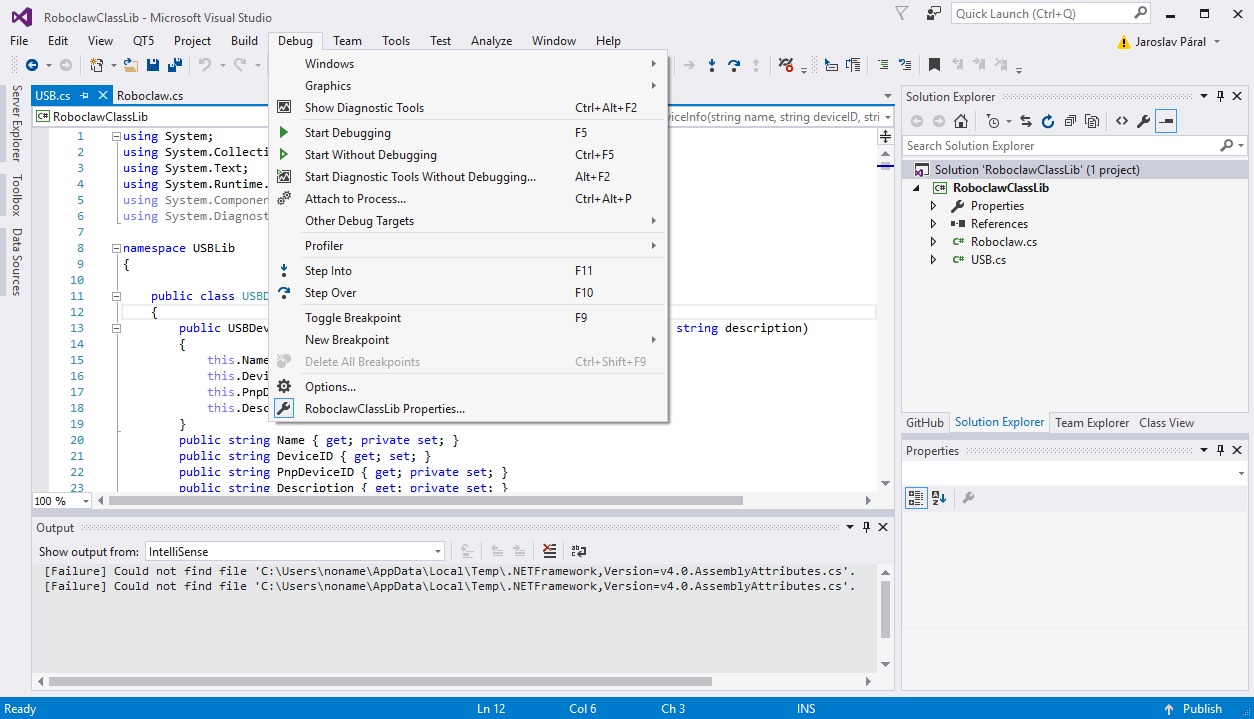
\includegraphics[width=\textwidth]{images/visual-studio_debug.png}
    \caption[Ukázka prostředí v~Microsoft Visual Studio Community 2015]{Ukázka prostředí v~Microsoft Visual Studio Community 2015 \\
    Aby uživatel spustil program, musí vybrat volbu \texttt{Start Without Debugging}, což je v~pořadí až druhá volba a~začátečník ani nemusí tušit, co znamená slovo debugging. 
    }
    \label{fig:visual-studio-community-2015}
\end{figure}

\begin{figure}[h]
    \centering
    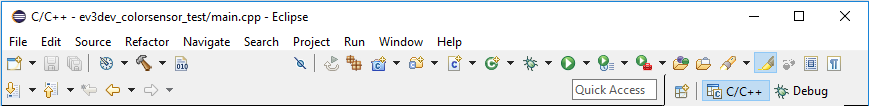
\includegraphics[width=\textwidth]{images/eclipse_tools-panel_focus.png}
    \caption[Ukázka panelu nástrojů v~prostředí Eclipse]{Ukázka panelu nástrojů v~prostředí Eclipse \\
    Zkuste vysvětlit skupině 15 začátečníků, kterou ikonku mají zmáčknout pro překlad, a~kterou pro spuštění. S~velkou pravděpodobností to polovina udělá poprvé špatně.  
    }
    \label{fig:eclipse_tools-panel}
\end{figure}

\subsection{Arduino IDE a~Processing}



Na opačné straně vývojářských nástrojů stojí programy Arduino IDE~\cite{arduino-web} a~Processing~\cite{processing-web} (stále kategorie~C).

Arduino IDE je vývojářský nástroj pro open-source elektronickou platformu Arduino, s~kterou lze jednoduše sestavovat hardware a~programovat software.
To vše bez potřeby drahého vybavení a~hlubších znalostí programování a~mikroprocesorů. 
Platforma využívá převážně mikrokontroléry AVR od firmy Atmel.
Jako programovací jazyk se používá Wiring~\cite{arduino-wiring}, který vychází z~jazyka C.

Processing je taktéž open-source vývojářský program, ale i~jazyk, určený pro snadnou tvorbu vizuálně zajímavé a~interaktivní grafiky.
Vznikl v~rámci MIT Media Lab~\cite{processing-web_overview} jako nástroj pro umělce a~lidi, kteří chtějí tvořit elektronické umění, ale nejsou programátoři.
Proto bylo hlavním cílem vytvořit jednoduché prostředí, které jim to umožní. Jazyk Processing je postaven nad Javou.

Arduino na Processing navázalo a~snaží se tuto myšlenku rozšířit na hardware. 
Zároveň použilo vývojářský program od Processingu a~upravilo jej pro své potřeby. 
V~mnoha oblastech se tyto dva projekty doplňují. 
Například lze pomocí Processingu graficky vizualizovat naměřené hodnoty ze senzorů připojených k~Arduinu.

Podle mého názoru nabízejí začátečníkovi přesně to co potřebuje: jednoduché UI, v~kterém se rychle zorientuje a~hned najde základní komponenty potřebné k~práci (hlavně tlačítka pro překlad a~spuštění programu). 
Vše si lze prohlédnout na obrázcích~\ref{fig:arduino+processing} a~\ref{fig:arduino-ide_tools-panel}.

\begin{figure}[h]
    \centering
    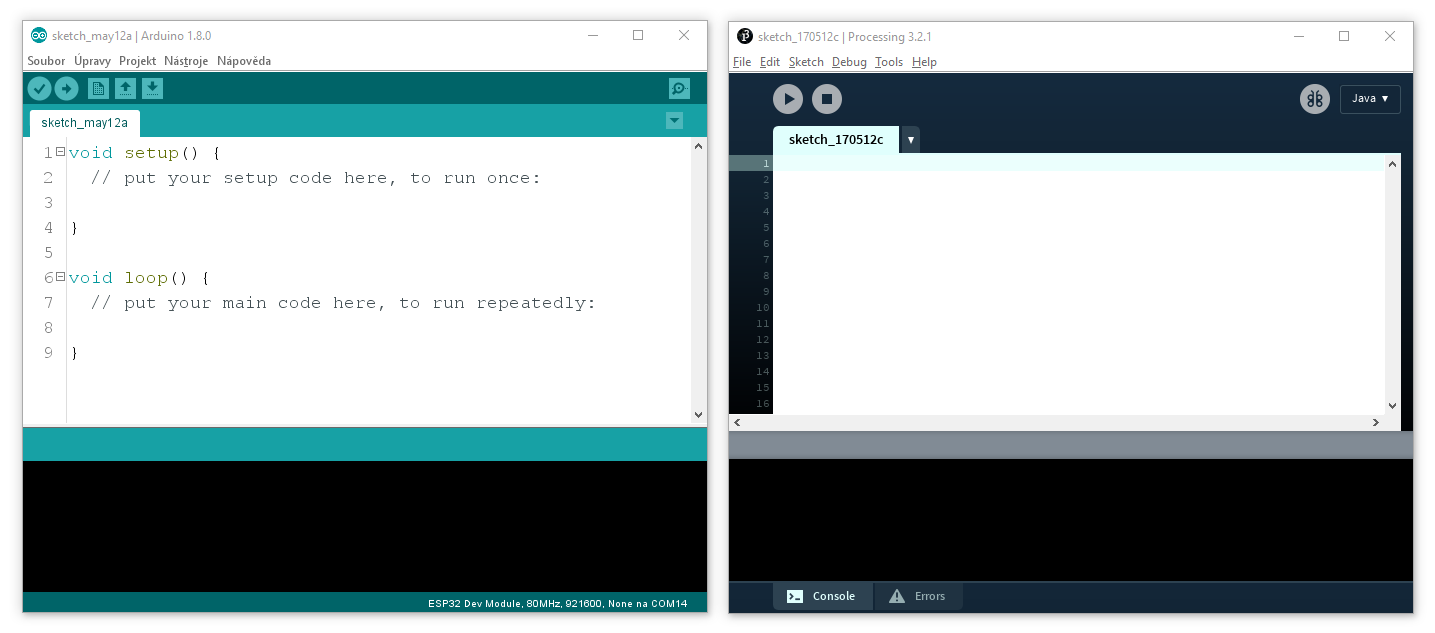
\includegraphics[width=\textwidth]{images/arduino+processing.png}
    \caption[Ukázka jednoduchých prostředí Arduino IDE a~Proccessing]{Ukázka jednoduchých prostředí Arduino IDE a~Proccessing \\
    Základní ovládací prvky potřebné při vývoji programů (tlačítka pro přeložení a~spuštění programu) jsou jasně a~zřetelně na očích a~neztrácejí se v~mnoha dalších ikonkách.}
    \label{fig:arduino+processing}
\end{figure}

\begin{figure}[h]
    \centering
    
\includegraphics[width=\textwidth]{images/arduino-ide_tools-panel.png}
    \caption{Panel s~nástroji v~Arduino IDE -- uživatel zde hned najde vše, co potřebuje}
    \label{fig:arduino-ide_tools-panel}
\end{figure}

I~tyto programy mají ale své problémy. 
Arduino IDE neumí našeptávat nebo zobrazovat nápovědu k~funkcím. 
Zároveň špatně zobrazuje chybové hlášky objevené při překladu.

Processing je na tom lépe. 
Má integrovaný základní našeptávač. 
Dokonce zvládá ukazovat datové typy parametrů.
Nezobrazuje však už jejich název, tudíž většinou nelze určit, co za parametr se očekává.
Lépe je v editoru zapracováno i~vypisování chyb a~je možné zapnout i~kontrolu správnosti kódu v průběhu psaní.

Bohužel tato IDE jsou šitá na míru daným platformám a~proto je nelze v~rámci mé práce využít. 
Poslouží ale jako dobrá inspirace pro výběr vhodného editoru.

\subsection{Visual Studio Code}


Po vyzkoušení výše zmíněných IDE jsem se rozhodl vrátit ke~kategorii~B a vyzkoušet nový editor Visual Studio Code. 
Jedná se o~relativně čerstvý počin Microsoftu, který tento editor představil v~rámci BUILDu 2015~\cite{visual-studio-code_initial-release}.


Visual Studio Code (dále jen VS Code) je zdarma dostupný multiplatformní (Windows, Linux, Mac) open-source editor s~integrovaným našeptáváním, Gitem a~podporou doplňků a~skriptování.
Probíhá u~něj velmi rychlý vývoj a~aktuálně jej lze považovat za jeden z~nejlepších editorů v~této kategorii.
V mnoha ohledech již předčil své konkurenty (editor Atom a~Sublime).
Například ve~srovnání s~Atomem je výrazně rychlejší.

Oproti vývojovým IDE z~kategorie~C má dle mého názoru značně jednoduší UI, při zachování rozsáhlých možností rozšiřování a~pokročilých funkcí. 
Základní funkce jsou dostupné přes nabídku v~horní a~boční liště. 
Všechny ostatní funkce lze najít přes speciální příkazovou řádků, která se spouští klávesovou zkratkou \texttt{Ctrl+Shift+P}. 
Tato příkazová řádka je ale běžnému uživateli skrytá a~tak jej neruší při používání.
Díky tomu nabízí VS~Code velké množství funkci při zachování jednoduchého uživatelského rozhraní.

\begin{figure}[h]
    \centering
    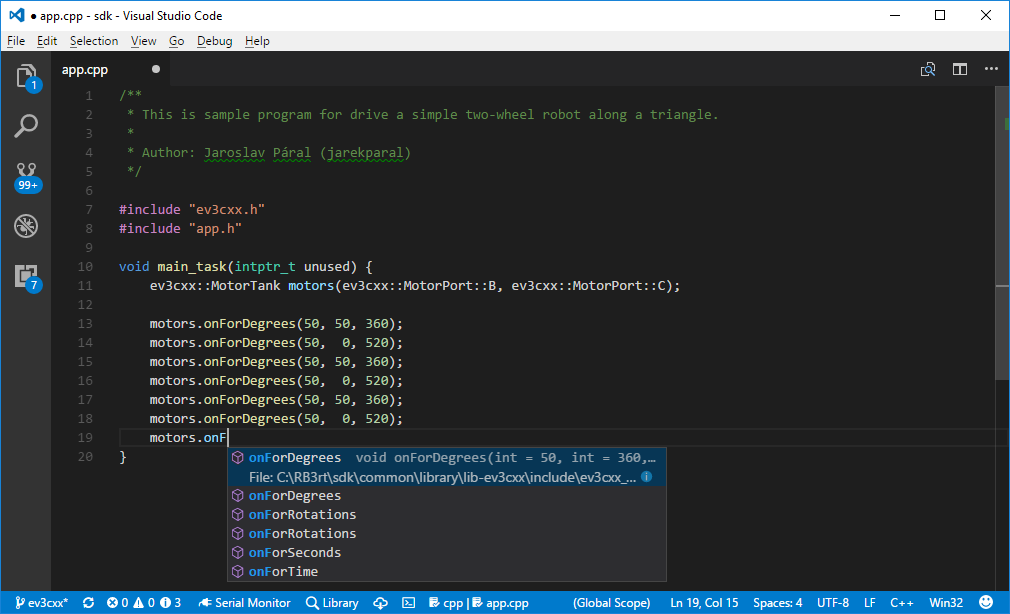
\includegraphics[width=\textwidth]{images/visual-studio-code_intellisense-function.png}
    \caption{Ukázka našeptávání ve Visual Studio Code -- doplňování názvu funkce}
    \label{fig:visual-studio-code_intellisense-function}
\end{figure}


Do VS~Code je možné nainstalovat celou řadu rozšíření. 
Tím nejzajímavější je doplněk  \texttt{C/C++ for Visual Studio Code}~\cite{vs-code_cpptools} přímo od~Microsoftu, který nabízí velmi dobré našeptávání, automatické formátování nebo vyhledávání definic a~symbolů.
Tato funkcionalita například velmi chybí v~Arduino IDE, na což si většina mých studentů v~kurzech stěžuje, když zjistí, že ji jiný nástroj umí.

Dalšími důležitými funkcemi jsou integrovaný terminál a~možnost jednoduchého spouštění skriptů.
VS~Code také nabízí snadné nadefinování klávesových zkratek, s~jejichž pomocí lze volat vlastní skripty.
Touto cestou jsem se rozhodl implementovat překlad uživatelských programů a~následné zasílání programu do~EV3.
K veškeré činnosti uživateli stačí jen tři klávesové zkratky: přeložení programu (\texttt{F5}), odeslání programu (\texttt{F6}) a~kombinace předchozích dvou příkazů v~rámci jedné klávesy (\texttt{F7}).
Zároveň jsem předpřipravil zkratku \texttt{F8} pro spuštění aplikace Lorris s integrovaným terminálem pro komunikaci přes Bluetooth a \texttt{F9} pro otevření webových stránek s dokumentací.


\section{Zprovoznění prostředí}

Vývojové prostředí se skládá z editoru, kompilátoru, EV3RT systému, knihoven, skriptů a bootovatelné image systému, určené ke spouštění na \brick{\it u}.
V následujících dvou podkapitolách bude probrán postup na zprovoznění celého prostředí.

\subsection{Instalace editoru, překladače a nahrání programu do \brick{\it u}}

Pro překlad a nahrání programu do systému EV3RT na Windows je potřeba nainstalovat následující software:

\begin{itemize}
    \item Cygwin (s balíčky make, perl, diffutil, gcc-core, gcc-g++, curl a libboost-devel)
    \item GCC překladač pro procesory ARM -- gcc-arm-none-eabi
    \item Visual Studio Code s doplňkem C/C++ for Visual Studio Code
\end{itemize}

Abych uživateli a případně učitelům usnadnil instalaci a konfiguraci celého prostředí, připravil jsem batch skript, který všechen potřebný software stáhne a postupně nainstaluje.
Skript vyžaduje administrátorská práva a občasnou interakci uživatel.
Součástí skriptu je i stažení systému EV3RT s C++ API a šablona se vzorovým projektem pro uživatele. 
Aktuálně je vyžadováno fixní umístění softwaru Cygwin a prostředí pro EV3RT do kořenového adresáře disku C.

Po instalaci si již může uživatel nakopírovat vzorový projekt, který je uložený ve složce \texttt{C:/RB3rt-projekt}, kam uzná za vhodné. 
Otevřít jej ve VS Code, nastavit klávesové zkratky a začít programovat.
Pokud chce svůj kód přeložit, stačí zmáčknout klávesu \texttt{F5}. 
Tím se zavolá přepřipravený skript, který spustí kompilaci přes Makefile v Cygwinu. 
Jelikož jsem musel vyřešit propojení kompilace v Cygwinu s VS Code, kopíruji vždy uživatelův projekt do adresáře se systémem EV3RT, kde následně probíhá samotný překlad.

Celý průběh překladu vidí uživatel v  terminálu, který je součástí VS~Code. 
Pokud se vyskytne jakákoliv chyba, je o~ní uživatel informován přes zmíněný terminál.
Při úspěšném přeložení lze následně zkompilovanou aplikaci nahrát na \EVbrick{}. 
První možností, jak nahrát aplikaci do systému je za pomocí USB. \brick{} s EV3RT se při propojení s PC přes USB kabel chová jako USB Mass Storage zařízení připojit k počítači a lze s ním pracovat jako se standardní SD kartou.
Další možností, většinou komfortnější, je využít integrovaný Bluetooth. 
Přes něj lze zasílat aplikace do systému a zároveň komunikovat s programem. 
EV3RT nabízí dva módy nahrávání přes Bluetooth: SPP\footnote{SPP = Serial Port Profile}, standardní sériový port a PAN\footnote{PAN = Personal Area Network}, v kterém se EV3RT chová jako síťové zařízení.

Z pohledu používání je lepší volba PAN módu, protože nekoliduje s SPP módem v uživatelských aplikacích. 
V rámci obsluhy Bluetooth, při programování vlastních aplikací, má uživatel dostupný jen SPP mód.
Proto pro odesílání aplikací využívám právě PAN a uživatel ve VS~Code spustí odeslání  pomocí klávesy \texttt{F6} (případně pokud chce program přeložit a hned odeslat, může použít klávesu \texttt{F7}).
Před tím, než může ale uživatel nahrát program do EV3RT, je potřeba se na \brick{\it u}, v menu systému, přepnout do režimu příjmu aplikace přes PAN.

\subsection{Nahrání systému EV3RT do EV3}

Pro provozování EV3RT na \brick{\it u} je potřeba nahrát image systému na micro SDHC kartu (minimální velikost musí být 4~GB -- EV3RT podporuje jen SDHC karty).
\EVbrick{} umožňuje spouštění systémů i z SD karty. Tento režim lze přirovnat k dual-bootu na PC. 
Výhodou je, že tím nehrozí zničení originálního systému a je možné velmi rychle přecházet mezi EV3RT a LEGO systémem. 
Musíte jen vložit SD kartu s EV3RT a nastartovat jej nebo naopak vypnout EV3RT, vyjmout kartu a spustit původní systém.

Image systému se automaticky stáhla v rámci instalace vývojové prostředí, popsané v předchozí kapitole, do složky \texttt{C:/RB3rt-image}. 
Uživatel jen musí veškerý obsah daného adresáře nakopírovat na micro~SDHC kartu a následně ji vložit do \brick{\it u}.


\section{Dokumentace}

Dokumentace k vývojovému prostředí lze rozdělit na dvě varianty. 
První varianta jsou komentáře ve zdrojovém kódu se syntaxí Doxygenu.
Tuto dokumentaci jsem tvořil pro pokročilejší uživatele, kteří by například chtěli rozšiřovat funkčnost C++~API. 
Zároveň je tvořená v angličtině a tudíž může posloužit lidem z celého světa.
Dokumentace je automaticky generovaná a je součástí repozitáře s API~\cite{roboticsbrno-EV3RT-API-Reference}.
     
Druhou variantou, která je primárně určená pro české uživatele tvořím za pomocí značkovacího jazyku RestructuredText~(reSt) a webové službu Read The Docs~\cite{readthedocs}.
Dokumentace je díky této službě dostupná jak online~\cite{readthedocs-rb3rt}, tak ji lze stáhnout v PDF formátu nebo HTML pro offline používání.
Pomocí obrázků programových bloku z LEGO softwaru ukazuji spojitost se svým objektovým API a LEGO bloky.
Součástí textů je i krátký tutoriál, který uživatele seznámí v několika lekcích se základními komponentami z \legoEV{} a jejich ekvivalenty v C++ API. 
V rámci jednotlivých úkolů si je uživatel prakticky vyzkouší.
Ukázku dokumentace lze najít v příloze.





\section{Dokumentace}

Dokumentace k vývojovému prostředí lze rozdělit na dvě varianty. 
První varianta jsou komentáře ve zdrojovém kódu se syntaxí Doxygenu.
Tuto dokumentaci jsem tvořil pro pokročilejší uživatele, kteří by například chtěli rozšiřovat funkčnost C++~API. 
Zároveň je tvořená v angličtině a tudíž může posloužit lidem z celého světa.
Dokumentace je automaticky generovaná a je součástí repozitáře s API~\cite{roboticsbrno-EV3RT-API-Reference}.
     
Druhou variantou, která je primárně určená pro české uživatele, tvořím za pomocí značkovacího jazyku RestructuredText~(reSt) a webové službu Read The Docs~\cite{readthedocs}.
Dokumentace je díky této službě dostupná jak online~\cite{readthedocs-rb3rt}, tak ji lze stáhnout v PDF formátu nebo HTML pro offline používání.
Pomocí obrázků programových bloku z LEGO softwaru ukazuji souvislost mezi objektovým C++ API a LEGO bloky.
Součástí textů je i krátký tutoriál, který uživatele seznámí v několika lekcích se základními komponentami z \legoEV{} a jejich ekvivalenty v C++ API. 
V rámci jednotlivých úkolů si je uživatel prakticky vyzkouší.

\section{Testování se studenty}

V rámci testování celého prostředí jsem začal zkoušet používat objektové API se studenty na SPŠ a VOŠ Brno, Sokolská, kde vedu robotický kroužek.
Studenti mají k dispozici již přes rok stavebnice \legoEV{} a za tuto dobu jsem s nimi již absolvoval několik soutěží. 
Někteří z nich se s programováním setkali poprvé až v LEGO softwaru.
Část ale měla již předchozí zkušenosti v jiných programovacích jazycích (C/C++, Java).

Testování probíhalo tak, že studenti dostali půl hodiny na prostudovaní dokumentace k C++ API na Read The Docs~\cite{readthedocs}. 
Během této doby pokládali dotazy, s tím co jim nebylo jasné. 
Většinou se jednalo o nedostatečně vysvětlenou oblast v API. 

Následně jsem studentům postupně zadával řešení jednotlivých úkolů, které jsou zpracovány v rámci Robotutoriálu  na Read The Docs~\cite{readthedocs}.
Studenti tak zkoušeli základní činnosti jako objet s robotem trojúhelník, nakreslit s ním domeček, dojet k překážce  a odvézt jí. 
Finálním úkolem byla jízda po čáře.
Ke každému příkladu bylo předpřipraveno i vzorové řešení, jak v LEGO blocích, tak C++ API.
Pokud si studenti nevěděli rady, mohli se podívat na řešení. 
Dle pozorování ovšem skoro nikdo vzorová řešení nevyužil a zvládali požadované úkoly jen s dokumentaci k jednotlivým třídám a metodám.
Prakticky to brali jako výzvu, kdo první zvládne naprogramovat daný úkol aniž by se díval na řešení.

Při těchto jednoduchých úkolech nedělalo studentům problém s C++ API pracovat a bylo vidět, že jim podobnost s LEGO bloky velmi pomáhá.
V rámci rozsáhlosti testovacích úkolů (v optimálním případě byl zdrojový kód vždy do 15 řádků v hlavní funkci) jsme nemohli otestovat přehlednost a srozumitelnost kódu při rozsáhlejších projektech v porovnání s LEGO bloky.
Aktuálně ale mají studenti API k dispozici a plánují jej využít k programování robota na soutěž Ketchup House v rámci Robotického dne 2017 v Praze.
Během této doby budu se studenty dále pokračovat na rozvoji API, tak aby jim co nejlépe vyhovovalo.
Již teď si ale myslím, že celé prostředí lze běžně využívat k programování \legoEV{}.

  
  \chapter{Závěr}

Práce zpracovává rešerši na dostupné vývojové platformy v~rámci výuky programování na \legoEV{}.
Z~výsledků rešerše vyplynulo, že nejvhodnější systém pro EV3 je RTOS EV3RT. 
Hlavními důvody jsou výkonost, real-timovost, otevřený zdrojový kód, snadná modifikovatelnost a~dostupnost pro uživatele na všech běžných operačních systémech (Windows, Mac, Linux).

RTOS EV3RT byl výkonnostně porovnán se standardním systémem v~\EVbrick{\it u} rozsáhlou sadou testů.
Výsledky ukazují výrazný výkonnostní rozdíl při provádění jednotlivých činností. 
EV3RT překonává \lego{} systém ve většině oblastí v~rozmezí sto až tisíci násobku.
% Zároveň je u něj zajištěno velmi přesné časování a nedochází u něj k časovým prodlevám 
Z~těchto důvodů byl RTOS EV3RT vybrán jako vhodný systém pro výuku programování. 

Práce se dále věnuje návrhu vývojového prostředí. 
Vybírá požadavky, které budou u~daného prostředí prioritou.
Pro EV3RT práce zpracovává objektově orientované C++~API s~anglickou dokumentací, které pokrývá kompletní funkcionality \legoEV{}. 
API bylo vyvinuto s~důrazem na jednoduchý přechod z~obrázkového LEGO Softwaru a~proto by pro uživatele mělo být snadné začít v~něm programovat.
To se také potvrdilo během testování se studenty.

Byl proveden i~průzkum několika vývojářských editorů. 
Za nejvhodnější pro začátečníky v~programování byl zvolen Visual Studio Code, kvůli svému jednoduchému UI, které zároveň zachovává rozsáhlé možností přizpůsobení, velkou palety doplňků a~kvalitní našeptávání. 

K~celému prostředí je připravená česká dokumentace. 
Pro uživatele je připraven popis C++~API i~vývojářského editoru. 
Pro každou oblast používání je zpracováno přehledné přirovnání jednotlivých funkcí s~LEGO Softwarem.
Žáci SPŠ a~VOŠ Brno, Sokolská již postupně toto prostředí začínají využívat k~programování.
Během testování s~nimi byli odhaleny některé nedostatky v~dokumentaci a~pojmenování metod v~API. 
Jinak si ale studenti prostředí i~API pochvalovali. 
Za jednu hodinu si zvládli projít dokumentaci a~začít programovat. 
Díky podobnosti API s~LEGO Softwarem jim nedělalo problém psát ekvivalentní programy.
Aktuálně probíhají průběžné úpravy dle zpětné vazbu studentů.

Celé prostředí je momentálně připraveno k~plnému využívání s~\legoEV{}. 
I~tak je tu mnoho oblastí, ve kterých jej lze dále rozvíjet. 
Rozpracovány jsou tutoriály se složitějšími úlohami pro studenty, na kterých by se mohli naučit další činnosti (programování více souběžných tasku, vytváření PID regulátorů, rozsáhlejší loggování do souborů).
V~budoucnu je i~plánu přidání další vrstvy v~API pro jednoduché zakomponování činností jako práce se souřadnicemi, plánování trasy nebo herní logika.


  
  
  
  %\chapter{Osnova práce}
\section{Úvod}
\section{Historie LEGO MINDSTORMS}
\section{Dostupné platformy pro programování EV3}
\section{?Testování platforem}
\section{EV3RT}
\section{Rozvoj EV3RT}
\section{Závěr}
    	
  % Pouzita literatura / Bibliography
  % ----------------------------------------------
\ifslovak
  \makeatletter
  \def\@openbib@code{\addcontentsline{toc}{chapter}{Literatúra}}
  \makeatother
  \bibliographystyle{bib-styles/czechiso}
\else
  \ifczech
    \makeatletter
    \def\@openbib@code{\addcontentsline{toc}{chapter}{Literatura}}
    \makeatother
    \bibliographystyle{bib-styles/czechiso}
  \else 
    \makeatletter
    \def\@openbib@code{\addcontentsline{toc}{chapter}{Bibliography}}
    \makeatother
    \bibliographystyle{bib-styles/englishiso}
  %  \bibliographystyle{alpha}
  \fi
\fi
  \begin{flushleft}
  \bibliography{projekt-20-literatura-bibliography}
  \end{flushleft}

  % vynechani stranky v oboustrannem rezimu
  % Skip the page in the two-sided mode
  \iftwoside
    \cleardoublepage
  \fi

  % Prilohy / Appendices
  % ---------------------------------------------
  \appendix
\ifczech
  \renewcommand{\appendixpagename}{Přílohy}
  \renewcommand{\appendixtocname}{Přílohy}
  \renewcommand{\appendixname}{Příloha}
\fi
\ifslovak
  \renewcommand{\appendixpagename}{Prílohy}
  \renewcommand{\appendixtocname}{Prílohy}
  \renewcommand{\appendixname}{Príloha}
\fi
%  \appendixpage

% vynechani stranky v oboustrannem rezimu
% Skip the page in the two-sided mode
%\iftwoside
%  \cleardoublepage
%\fi
  
\ifslovak
%  \section*{Zoznam príloh}
%  \addcontentsline{toc}{section}{Zoznam príloh}
\else
  \ifczech
%    \section*{Seznam příloh}
%    \addcontentsline{toc}{section}{Seznam příloh}
  \else
%    \section*{List of Appendices}
%    \addcontentsline{toc}{section}{List of Appendices}
  \fi
\fi
  \startcontents[chapters]
  \setlength{\parskip}{0pt}
  % seznam příloh / list of appendices
  % \printcontents[chapters]{l}{0}{\setcounter{tocdepth}{2}}
  
  \ifODSAZ
    \setlength{\parskip}{0.5\bigskipamount}
  \else
    \setlength{\parskip}{0pt}
  \fi
  
  % vynechani stranky v oboustrannem rezimu
  \iftwoside
    \cleardoublepage
  \fi
  \chapter{Obrázky}

\begin{figure}[h]
	\centering
	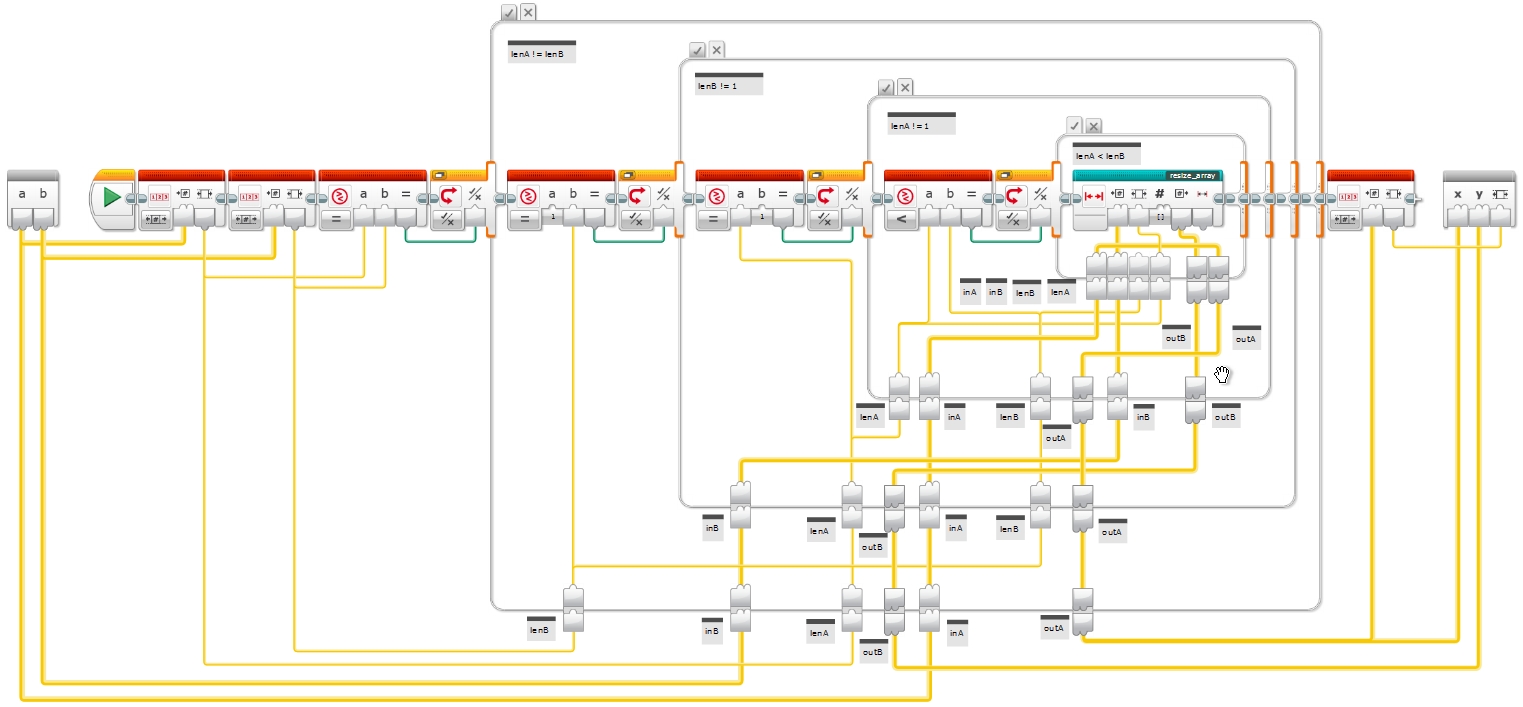
\includegraphics[angle=-90,origin=c,width=280px]{images/lego-soft_legolib_match_array_length.png}
	\caption[Předávání hodnot v \legoSW{}]{Předávání hodnot v \legoSW{}}
	\label{fig:lego-soft_legolib_match_array_length}
\end{figure}




 % viz. prilohy.tex / see prilohy.tex
\end{document}
